\documentclass[12pt]{article}
\usepackage[utf8]{inputenc}
\usepackage{fancyhdr}
\usepackage{lastpage}
\renewcommand{\baselinestretch}{1.5}
\usepackage{float}

\usepackage{hyperref}
\usepackage{tikz} 
\usetikzlibrary{shapes,arrows.meta,calc}

\usepackage[margin=3cm]{geometry}
\usepackage{amssymb}
\usepackage{amsthm}
\usepackage{amsmath}
\usepackage{pgfgantt}
\graphicspath{{img/}{../img/}}

\usepackage{pgfplots, pgfplotstable}
\pgfplotsset{compat=newest}
\usepgfplotslibrary{colormaps}
\usepackage{xstring}
\usepackage{xcolor}
\usepackage{caption}
\usepackage{setspace}
\usepackage{subcaption}
\definecolor{armygreen}{rgb}{0.29, 0.33, 0.13}

\pagestyle{fancy}
\fancyhf{}
\fancyfoot[C]{\thepage}


\usepackage[numbers]{natbib}

\usepackage{listings}
\lstset{
  basicstyle=\ttfamily,
  columns=fullflexible,
  frame=single,
  breaklines=true,
  postbreak=\mbox{\textcolor{red}{$\hookrightarrow$}\space},
}

\begin{document}
\begin{titlepage}
    \centering
    \vspace*{1cm}

    
    
    
\includegraphics[width=0.3\textwidth]{crest}

    \vspace{1.5cm}
    \Large
    \textbf{SIMULATING THE EMERGENT AUTONOMOUS BEHAVIOUR OF UNMANNED AERIAL VEHICLE SWARMS}

    \vspace{1cm}

    by

    \vspace{1cm}
    
    \textbf{ANTONIO BRITO}
    
    \vfill
    \Huge
    \textcolor{red}{\textbf{SECOND DRAFT}}

    \vfill
    \Large
    Supervised by Nathan Griffiths
    
    
    \vspace{1.5cm}
    
    \Large
    Department of Computer Science\\
    University of Warwick\\
    \the\year
    
\end{titlepage}
\tableofcontents
\newpage
% FOREWORD - DELETE
% \begin{center}
%     \Large
%     Foreword\\
%     \vspace{0.8cm}
%     \textcolor{red}{DRAFT ONLY}\\
%     \vspace{4cm}
%     \normalsize
% \end{center}
% This is a list of known issues and improvements that need to be made to the report as presented in the draft.
% \begin{enumerate}
%     \item Section \ref{sec:context} has overlap in both the introduction and background. This might need a rewrite.
%     \item The sensitivity analysis lacks substance - include more resolutions, Quant analysis, repeatability and further discussion on these results.
%     \item Include further discussion on swarm cooperation.
%     \item Keywords list and abbreviations/key terms list
% \end{enumerate}
% \newpage
% FOREWORD - DELETE
\thispagestyle{empty}
\listoffigures
\listoftables
\newpage

\begin{center}
    \vspace{0.8cm}
    \Large
    \textbf{SIMULATING THE EMERGENT AUTONOMOUS BEHAVIOUR OF UNMANNED AERIAL VEHICLE SWARMS}

    \large
    \vspace{0.8cm}
    \textbf{ANTONIO BRITO}

    \vfill
       
    \Large
    \textbf{Abstract}
    \vspace{2cm}
\end{center}
\onehalfspacing

Path planning and control algorithms for mobile robots, specifically unmanned aerial vehicles (UAVs), which typically fall under the A* family of algorithms, have been well explored\cite{IJSAEM,Chen}. Likewise, multi-agent pathfinding within the context of UAV systems has been explored, most notably by \citet{burwell_2019}.

Notably, early developments in the field of swarm robotics on ground vehicles had been made\cite{Monada}, with the focus shifting from ground vehicles to aerial vehicles in recent years. With this have come descriptions of the technical frameworks\cite{Zhou} and operational challenges of UAV swarms\cite{Verdoucq}.

This project will explore the feasibility of using a simpler, rule-based system to simulate emergent behaviour for control of UAVs, based on an extension of the principles of Reynolds' Boids\cite{Reynolds}.

We also explore the limitations of this approach, specifically in 3D, and explore an extension to our developed algorithm which focuses on local search and a potential field approach to path planning (Local Potential Field Emergence), to reduce complexity in the parameter space of the Boids algorithm.

Through this project, we aim to provide a proof of concept for the feasibility of emergent behaviour in UAV swarms and to provide a basis for further research in the field.

\vspace{2cm}

\noindent\textbf{Keywords:} Unmanned Aerial Vehicles, Swarm Robotics, Artificial Intelligence, Emergent Behaviour, Simulation, Function Optimisation, Artificial Potential Fields

\newpage

\section{Context}
\label{sec:context}
\subsection{Introduction}
\label{sec:introduction}
The use of unmanned aerial vehicles (UAVs) has been growing rapidly, with both civil and military applications. Namely, their ease of deployment, low maintenance cost, high mobility and ability to hover mean they are well suited to a variety of tasks, such as surveillance, reconnaissance, search and rescue, and logistics\cite{Hayat}.

Utilising multiple agents for these applications has several advantages. Firstly, it introduces redundancy into the system, allowing for effective fault tolerance, which is extremely vital in safety-critical applications\cite{Perez}. A recent example of this is the use of UAV swarms in forest fire monitoring\cite{Hu}.

Additionally, the ability to scale the number of agents in the swarm allows for greater efficiency in surveillance and reconnaissance tasks, as well as the ability to cover a larger area in search and rescue operations over a given period.

In Section \ref{sec:methodology}, we will explore tailoring the behaviour of our agents to simulate some scenarios, based on these expected applications of UAVs. To this end, we will explore the flexibility of UAV swarms in the context of adapting to different scenarios.

Implementations for the control and path planning of mobile robotics are well studied. Namely, A* and its variants are well studied and widely used for path planning in mobile robotics\cite{Chen}. Additionally, Particle Swarm Optimisation (PSO) has been used for path planning in UAV swarms\cite{Pyke}.

This project's focus will be on a simulated implementation of Reynolds' Boids\cite{Reynolds} algorithm, which is a rule-based system for simulating emergent behaviour in a flock of birds. It has been demonstrated that this algorithm can be used for effective autonomous control of swarms\cite{Basu}, but lacks in the ability for pathfinding and obstacle avoidance\cite{Pyke}. Hence, we will look to extend this autonomous control in a world-like environment, by implementing goal-seeking, terrain avoidance and obstacle avoidance as added behaviours.

The implementation of this algorithm will be in the context of a 3D environment, to provide a proof of concept for the feasibility of emergent behaviour in UAV swarms, based on optimising the influence of the behaviours in our algorithm to align to our expected applications of UAV swarms. We will explore issues with this approach, and propose an extension to our developed algorithm which modifies the behaviours of the agents to simulate an artificial potential field, which has been shown to be effective as a mobility model for UAV swarms\cite{Falomir}.

\subsection{Background}

The foundation of this proof of concept is anchored in the Unity game engine, known for its robust physics engine and comprehensive 3D environment capabilities. These features are instrumental for our simulation as they proficiently manage collisions, rigid body dynamics, and raycasting. The versatility of Unity is evident from its proven track record in handling complex agent-based simulations, which extends to sophisticated artificial intelligence tasks, including reinforcement learning \cite{juliani2020unity}. This versatility validates Unity as an apt platform for conducting extensive simulations required by this project.

Our project aims to advance the traditional two-dimensional Boids simulations used in UAV swarm control, as discussed by \citet{madey2013design}. Their work provides a comprehensive exploration of UAV swarm command and control strategies within a simulated environment. This paper offers valuable insights into the complexities of designing swarm behaviours that are not only autonomous but also capable of executing sophisticated tasks as a cohesive unit. The authors address both the potential and the challenges of UAV swarms in complex mission scenarios, making their research highly relevant to the development of 3D UAV swarm simulations. Their work extends the basic principles of Reynolds' Boids model, which uses simple rules to simulate flocking behaviour, by adapting these concepts to the operational needs of military UAV swarms. This adaptation is particularly relevant to our project, as we aim to extend two-dimensional Boids simulations into three-dimensional space, incorporating more complex dynamics such as quadcopter physics. 

Additionally, our approach involves an innovative integration of individual behavioural rules, following the methodologies outlined by \citet{watson}. This enhancement is expected to provide a more realistic and practical simulation framework that better mirrors real-world UAV operational dynamics. The incorporation of realistic dynamics, such as simplified realistic aircraft dynamics, into the flocking simulation represents a significant advancement over traditional point-mass models. This approach ensures that the simulated UAVs behave more like actual aircraft, accounting for factors like inertia and aerodynamic forces, which are crucial for creating more accurate and reliable simulations. The detailed exploration of rule weighting and its impact on flock dynamics provides a valuable framework for our project, particularly in how we might balance different behavioural influences to achieve desired swarm behaviours. \citet{watson} also emphasises the importance of developing meaningful statistical metrics to quantify flocking behaviour, an approach that could greatly enhance the analytical capabilities of our simulation. By understanding the relationships between rule weightings and flocking behaviour, we can more effectively tune our simulations to achieve specific operational goals or to mimic particular real-world scenarios.

To refine the effectiveness of the combined behavioural set, we employ simulated annealing as our optimisation technique. This probabilistic method is adept at approximating the global optimum of complex cost functions, making it particularly suitable for fine-tuning the behavioural weights within our algorithm to suit specific UAV swarm applications. 

In their study, \citet{Alaliyat2014OptimisationOB} present a comparative analysis of the optimisation of the Boids swarm model using Genetic Algorithms (GA) and Particle Swarm Optimisation (PSO). Their research, grounded in the application of these algorithms to enhance simulations of flocking behaviour, is both timely and relevant, particularly for real-time applications like video games and interactive simulations where computational efficiency is paramount.

The study implements the Boids model in Unity3D and optimises it using both GA and PSO. The results demonstrate that PSO not only achieves faster convergence but also maintains better computational efficiency compared to GA. This is attributed to PSO's mechanism of adjusting solutions based on both individual and social memory, which seems particularly suited to the dynamic interactions modelled in flocking behaviour.

Notably, both of these techniques present certain limitations when applied to behaviour space optimisation. Genetic algorithms, for instance, often require extensive computational resources and can be prone to premature convergence, potentially leading to suboptimal solutions. PSO, while efficient for continuous search spaces, can struggle with the discrete parameters typically found in UAV control settings. These issues underscore the challenges in behaviour optimisation and highlight the necessity for a nuanced approach that can adapt to the complexities of UAV swarm behaviour dynamics.

Our selection of simulated annealing over these methods is driven by its capability to escape local minima more effectively, thereby offering a greater probability of reaching a more comprehensive global solution. However, it's imperative to acknowledge the inherent challenges in employing this technique, such as the sensitivity to cooling schedules and the computational demands of evaluating multiple candidate solutions.

By building on established methodologies and integrating advanced optimisation techniques, this project seeks not only to extend the theoretical framework of UAV swarm simulations but also to provide actionable insights that could enhance practical implementations in real-world scenarios.


\newpage
\section{Physics Model}
Here, we will discuss the physics model of our simulation, which is comprised of the agents that make up the flock and each agent's interactions with the surrounding environment. We will also discuss the control system for the agents; how they handle inputs and how they move in response to these inputs.

We first note the environment in which the agents will be operating, which is comprised of a three-dimensional coordinate space, representing the global reference frame. The coordinate axes of this space are $x$, $y$ and $z$, representing north, up and east respectively.

\subsection{Agent}
We define an agent as a single unit within the simulation, which is capable of movement and interaction with the environment. The agent is capable of moving in three dimensions, with the ability to move north, south, east, west, up and down. The principal axes of an agent's movement are \emph{pitch}, along the transverse ($z$) axis, \emph{roll}, along the longitudinal ($x$) axis, and \emph{yaw}, along the vertical ($y$) axis.

We define the agent as an unmanned aerial vehicle (UAV), which can be modelled as a rigid body with mass $m$, on Earth. As such, gravity acts on the agent at $9.81\frac{m}{s^2}$. The drag coefficient is estimated at $0.975$ considering the mass of the body \cite{Hattenberger}. The dimensions and characteristics of the agent have been determined using both realistic averages \cite{Figliozzi} and estimations. These can be seen in Fig. \ref{fig:dimensions}.

\begin{figure}[ht]
    \centering
    \begin{tabular}{| c | c |} 
    \hline
    Parameter & Value \\ 
    \hline
    Mass, $m$ & 10 kg \\
    \hline
    Length, $l$ & 0.7 m \\
    \hline
    Width, $w$ & 0.7 m \\
    \hline
    Height, $h$ & 0.25 m \\
    \hline
    Propeller Area, $A$ & 0.16 m$^2$ \\
    \hline
    Distance To Propeller Centre, $d$ & 0.5 m \\
    \hline
    Drag Coefficient, $C_d$ & 0.975 \\
    \hline
    \end{tabular}
    \caption{Dimensions of the Agent}
    \label{fig:dimensions}
\end{figure}

The agent is modelled as a quadcopter, with four propellers that can be independently controlled to affect the movement of the agent. \citet{Thamm} notes that quadcopters are the most common type of UAV, due to their simplicity in design and control, as well as their ability to hover and manoeuvre in tight spaces, owing to their ability to rotate about their principal axes. For this reason, we have chosen to model our agent as a quadcopter.    

The body diagram of the quadcopter is shown in Fig. \ref{fig:quadcopter} alongside the local axes of movement. The agent as modelled in Unity is shown in Fig. \ref{fig:quadcopter-unity} with the same axes.

\begin{figure}[ht]
    \centering
    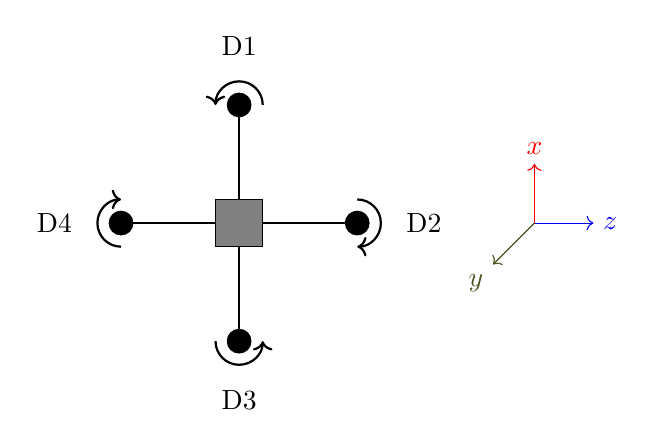
\begin{tikzpicture}[scale=1.5]
        % Coordinate system
        % \draw[->] (0,0) -- (1,0) node[right=1cm] {$z$};
        % \draw[->] (0,0) -- (0,1) node[above=1cm] {$x$};
        % \draw[->] (0,0) -- (-0.6,-0.6) node[below left] {$y$};
        
        % Quadrotor body
        \draw[fill=gray] (-0.2,0.2) rectangle (0.2,-0.2);
        
        % Arms
        \draw[thick] (-0.2,0) -- (-1,0);
        \draw[thick] (0.2,0) -- (1,0);
        \draw[thick] (0,0.2) -- (0,1);
        \draw[thick] (0,-0.2) -- (0,-1);

        % Axes
        \draw[->,red] (2.5,0) -- (2.5,0.5) node[above] {$x$};
        \draw[->,blue] (2.5,0) -- (3,0) node[right] {$z$};
        \draw[->,armygreen] (2.5,0) -- (2.15,-0.35) node[below left] {$y$};
        
        % Rotors with labels and direction
        % D1
        \draw[fill=black] (-1,0) circle (0.1) node[left=0.5cm] {D4};
        \draw[->,thick] (-1,-0.2) arc (270:90:0.2);
        % D2
        \draw[fill=black] (1,0) circle (0.1) node[right=0.5cm] {D2};
        \draw[->,thick] (1,0.2) arc (90:-90:0.2);
        % D3
        \draw[fill=black] (0,1) circle (0.1) node[above=0.5cm] {D1};
        \draw[->,thick] (0.2,1) arc (0:180:0.2);
        % D4
        \draw[fill=black] (0,-1) circle (0.1) node[below=0.5cm] {D3};
        \draw[->,thick] (-0.2,-1) arc (180:360:0.2);
    \end{tikzpicture}
    \caption{Quadcopter Body Diagram in the x-z plane}
    \label{fig:quadcopter}
\end{figure}

\begin{figure}[ht]
    \centering
    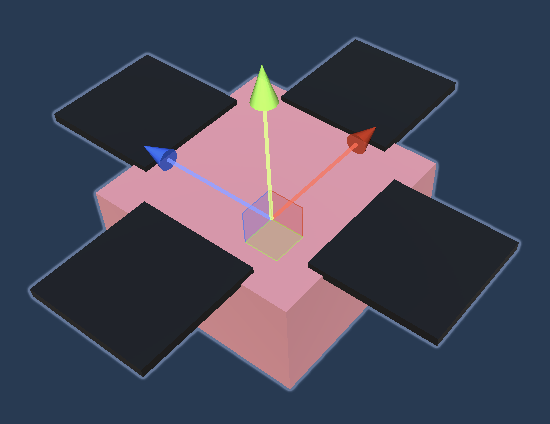
\includegraphics[height=80px]{agent}
    \caption{Agent in Unity}
    \label{fig:quadcopter-unity}
\end{figure}

We can control the agent's movement by adjusting the pitch, roll and yaw angles, as well as the thrust level of the agent's propellers. We define these as:

\begin{itemize}
    \item Roll angle (in radians), $\psi$
    \item Pitch angle (in radians), $\theta$
    \item Yaw rate (in $\frac{rad}{s}$), $\phi$
    \item Vertical thrust (in Newtons), $T$
\end{itemize}


For simplicity, these can be solely controlled by combinations of propeller thrust levels. A base thrust level, $T_b$, can be defined, which is the minimum thrust level required to maintain a stable hover. This is the thrust level required to counteract gravity, such that $T_b = mg$. For each control operation, $T_b$ can be augmented by a thrust level, $T_{add}$, such that $|T_{add}| < T_b$, which is the additional thrust required to perform the operation. As such, the control parameters can be operated by the following eight combinations of thrust levels for each propeller, with a high thrust level $T_{add} > 0$ and a low thrust level $T_{add} = 0$:


\begin{table}[ht]
    \begin{center}
    \begin{tabular}{| c | c | c |} 
    \hline
    Operation & High Thrust & Low Thrust \\ 
    \hline
    Positive Roll, $\psi_+$ & $D_4$ & $D_2$ \\
    \hline
    Negative Roll, $\psi_-$ & $D_2$ & $D_4$ \\
    \hline
    Positive Pitch, $\theta_+$ & $D_3$ & $D_1$ \\
    \hline
    Negative Pitch, $\theta_-$ & $D_1$ & $D_3$ \\
    \hline
    Positive Thrust, $T_+$ & $D_1, D_2, D_3, D_4$ & none \\
    \hline
    Negative Thrust, $T_-$ & none & $D_1, D_2, D_3, D_4$ \\
    \hline
    \end{tabular}
    \end{center}
    \caption{Control Operations and Thrust Levels}
    \label{tab:control}
\end{table}


It is noted that yaw is omitted from Table \ref{tab:control}. Within our simulation, the propellers do not rotate. This lends itself to needing a workaround for simulating yaw. In \emph{Unity}'s physics engine, the rotation of opposite propellers can be simulated by applying forces along the $x$ and $z$ axes. As such, yaw is simulated according to the values in Table \ref{tab:yaw-control}. The resultant forces are shown in Fig. \ref{fig:quadcopter-yaw}.

\begin{table}[ht]
    \begin{center}
    \begin{tabular}{| c | c | c |} 
    \hline
    Operation & Propeller & Direction of Force (respectively) \\ 
    \hline
    Positive Yaw, $\phi_+$ & $D_1, D_2$ & $Z_+, X_-$ \\
    \hline
    Positive Yaw, $\phi_+$ & $D_3, D_4$ & $Z_-, X_+$ \\
    \hline
    Negative Yaw, $\phi_-$ & $D_1, D_2$ & $Z_-, X_+$ \\
    \hline
    Negative Yaw, $\phi_-$ & $D_3, D_4$ & $Z_+, X_+$ \\
    \hline
    \end{tabular}
    \end{center}
    \caption{Yaw Directions and Respective Forces}
    \label{tab:yaw-control}
\end{table}

\begin{figure}[ht]
    \centering
    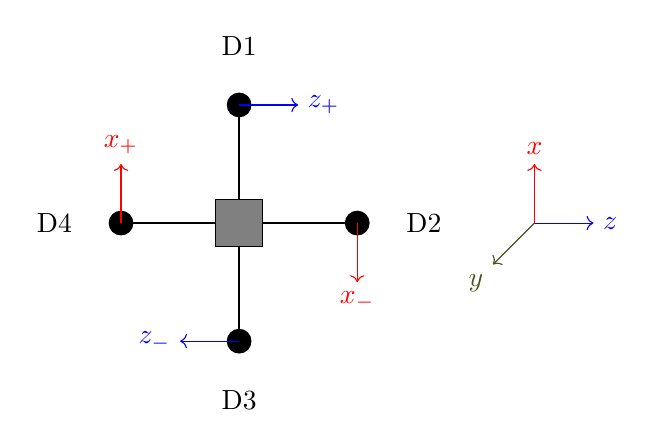
\begin{tikzpicture}[scale=1.5]
        % Coordinate system
        % \draw[->] (0,0) -- (1,0) node[right=1cm] {$z$};
        % \draw[->] (0,0) -- (0,1) node[above=1cm] {$x$};
        % \draw[->] (0,0) -- (-0.6,-0.6) node[below left] {$y$};
        
        % Quadrotor body
        \draw[fill=gray] (-0.2,0.2) rectangle (0.2,-0.2);
        
        % Arms
        \draw[thick] (-0.2,0) -- (-1,0);
        \draw[thick] (0.2,0) -- (1,0);
        \draw[thick] (0,0.2) -- (0,1);
        \draw[thick] (0,-0.2) -- (0,-1);

        % Axes
        \draw[->,red] (2.5,0) -- (2.5,0.5) node[above] {$x$};
        \draw[->,blue] (2.5,0) -- (3,0) node[right] {$z$};
        \draw[->,armygreen] (2.5,0) -- (2.15,-0.35) node[below left] {$y$};
        
        % Rotors with labels and direction
        % D1
        \draw[fill=black] (-1,0) circle (0.1) node[left=0.5cm] {D4};
        % \draw[->,thick] (-1,-0.2) arc (270:90:0.2);
        \draw[->,red] (-1,0) -- (-1,0.5) node[above] {$x_+$};
        % D2
        \draw[fill=black] (1,0) circle (0.1) node[right=0.5cm] {D2};
        % \draw[->,thick] (1,0.2) arc (90:-90:0.2);
        \draw[->,red] (1,0) -- (1,-0.5) node[below] {$x_-$};
        % D3
        \draw[fill=black] (0,1) circle (0.1) node[above=0.5cm] {D1};
        % \draw[->,thick] (0.2,1) arc (0:180:0.2);
        \draw[->,blue] (0,1) -- (0.5,1) node[right] {$z_+$};
        % D4
        \draw[fill=black] (0,-1) circle (0.1) node[below=0.5cm] {D3};
        % \draw[->,thick] (-0.2,-1) arc (180:360:0.2);
        \draw[->,blue] (0,-1) -- (-0.5,-1) node[left] {$z_-$};

    \end{tikzpicture}
    \caption{Propeller Forces for Positive (Clockwise) Yaw Control}
    \label{fig:quadcopter-yaw}
\end{figure}

In real-world physics, a couple of propellers could not provide thrust in both extremes of the same axes, as they could not switch rotation direction. Likewise, forces in adjacent propellers would not cause rotation in the same direction. However, for simplicity within the simulation, this is ignored. It is then possible to set some thrust constants for each control operation. An example assignment for the pitch and roll operations is seen below in Fig. \ref{tab:thrust-constants}.

\begin{table}[ht]
    \begin{center}
    \begin{tabular}{| c | c | c |} 
    \hline
    Thrust Level & Thrust ($N$) \\ 
    \hline
    High & $\frac{2m \cdot g}{4}$\\
    \hline
    Normal & $\frac{m \cdot g}{4}$\\
    \hline
    Low & $\frac{0.5m \cdot g}{4}$\\
    \hline
    \end{tabular}
    \end{center}
    \caption{Thrust Constants for a drone of mass $m$ kg}
    \label{tab:thrust-constants}
\end{table}

At this stage, we have a model for the control and movement of the agent. Input is given to the propeller controller, which outputs the thrust level as required in Fig. \ref{tab:thrust-constants} to the individual propellers, causing a rotation of the agent in the desired direction.


\subsection{Stabilisation}
\label{sec:stabilisation}

An issue arises with this implementation; the simulation becomes unstable as thrust cannot be provided in an accurate enough manner to counteract excessive rotation, notably in the roll and pitch axes. This can lead to the agent's rotation becoming overly large, causing it to roll over. If we consider an example input, represented by a single keypress to generate thrust to cause a pitch rotation, we can model the deviation from the desired pitch angle $\theta_{d} = 0.26$ over time, as shown in Fig. \ref{fig:pitch-angle}.

\begin{figure}[ht]
\centering
\begin{tikzpicture}
    \begin{axis}[
        xlabel={Time, $t$ (s)},
        ylabel={Deviation from $\theta_d$ (rad)},
        ymajorgrids=true,
        grid style=dashed,
        y dir=reverse,
        xmax=4
    ]
    \draw[thin] (axis cs:\pgfkeysvalueof{/pgfplots/xmin},0) -- (axis cs:\pgfkeysvalueof{/pgfplots/xmax},0);
    
    \addplot[
        color=blue,
        mark=none,
        ]
        table[col sep=comma, x=x, y=y] {pitchAngle.csv};
    
    \end{axis}
\end{tikzpicture}
\caption{Pitch angle due to input over time}
\label{fig:pitch-angle}
\end{figure}

Fig. \ref{fig:pitch-angle} shows that when given an input, the agent exceeds the desired pitch angle, crossing $\theta_d = 0$, then continues to rotate until it collides with the ground at $t \approx 2.2$ seconds. As such, the need for a control system becomes apparent, to mitigate the agent's desire to overshoot the desired angle.

\subsubsection{Proportional Controller}
A first intuition here is to control the rotation by reducing the thrust level as the agent approaches the desired angle, such that the thrust level at some time, $t$, is inversely proportional to the deviation from the desired angle as shown in Eq. \ref{eq:p-controller}.

\begin{equation}
    T_t \propto \frac{1}{\theta_d}
    \label{eq:p-controller}
\end{equation}

We can then define a proportionality constant, $K_p$ according to the inverse relationship in Eq. \ref{eq:p-controller}. Using different values for $K_p$, we can observe some behaviours in the deviation from the desired angle over time, as shown in Fig. \ref{fig:pitch-angle2}, which is split into two subfigures for clarity. The left-hand graph shows $K_p = 1$ and $K_p = 5$, and the right-hand graph shows $K_p = 5$ and $K_p = 10$.

\begin{figure}[ht]
    \centering
    \begin{subfigure}{.4\textwidth}
    \begin{tikzpicture}[trim axis left, trim axis right]
        \begin{axis}[
            xlabel={Time, $t$ (s)},
            ylabel={Deviation from $\theta_d$ (rad)},
            ymajorgrids=true,
            grid style=dashed,
            y dir=reverse,
            xmax=9
        ]
        \draw[thin] (axis cs:\pgfkeysvalueof{/pgfplots/xmin},0) -- (axis cs:\pgfkeysvalueof{/pgfplots/xmax},0);
        
        \addplot[
            color=blue,
            mark=none,
            line width=0.5mm,
            ]
            table[col sep=comma, x=x, y=y] {pcontrol1.csv};

        \addplot[
            color=red,
            mark=none,
            ]
            table[col sep=comma, x=x, y=y] {pcontrol5.csv};

            % \addplot[
            %     color=green,
            %     mark=none,
            %     ]
            %     table[col sep=comma, x=x, y=y] {pcontrol10.csv};
        
            \addlegendentry{$K_p = 1$};
            \addlegendentry{$K_p = 5$};
        
        \end{axis}
    \end{tikzpicture}
\end{subfigure}
\hfill
\begin{subfigure}{.4\textwidth}
    \begin{tikzpicture}[trim axis left, trim axis right]
        \begin{axis}[
            xlabel={Time, $t$ (s)},
            ymajorgrids=true,
            grid style=dashed,
            y dir=reverse,
            xmax=9
        ]
        \draw[thin] (axis cs:\pgfkeysvalueof{/pgfplots/xmin},0) -- (axis cs:\pgfkeysvalueof{/pgfplots/xmax},0);
        
        % \addplot[
        %     color=blue,
        %     mark=none,
        %     ]
        %     table[col sep=comma, x=x, y=y] {pcontrol1.csv};

        \addplot[
            color=red,
            mark=none,
            line width=0.2mm,
            ]
            table[col sep=comma, x=x, y=y] {pcontrol5.csv};

            \addplot[
                color=purple,
                mark=none,
                line width=0.3mm
                ]
                table[col sep=comma, x=x, y=y] {pcontrol10.csv};
        
                \addlegendentry{$K_p = 5$};
                \addlegendentry{$K_p = 10$};
        
        \end{axis}
    \end{tikzpicture}
\end{subfigure}
    \caption{Pitch angle due to input over time with proportional error correction}
    \label{fig:pitch-angle2}
    \end{figure}

As shown in Fig. \ref{fig:pitch-angle2}, we can see that adding a proportional controller to the system creates a steady state, as we can see that the limit of $\theta_d$ as $t \to \infty$ is $\approx 0$ in both graphs.

In the left-hand graph, we can see that increasing $K_p$ decreases the amount of deviation from the desired angle. However, in the right-hand graph, we can see that this increase becomes negligible at a point, and does not reach zero. Instead, we can observe some oscillations in this state, as the agent continually overshoots the desired angle, before correcting itself and overshooting again, to a lesser extent each time. In some sense, we require the agent's controller to predict overshooting the desired angle.

\subsubsection{Derivative Controller}

To predict overshooting the desired angle, we need to modify the controller to consider the rate of change of the deviation. A deviation that is changing rapidly (oscillating) will also have a large (but decreasing) rate of change of deviation. The aim is to reach a steady state; a deviation that is not changing over time, with a deviation of zero. Hence, we can aim to reduce this rate of change of deviation by adding a term to the controller that is proportional to the rate of change of deviation, namely, a derivative term. This is shown in Eq. \ref{eq:pd-controller}.

\begin{equation}
    T_t \propto \frac{1}{\theta_d} - K_d \frac{d\theta}{dt}
    \label{eq:pd-controller}
\end{equation}

As before, we can introduce a proportionality constant, $K_d$, to the derivative term. We can then observe the effect of this term on the deviation from the desired angle over time, as shown in Fig. \ref{fig:pitch-angle3}. We note that we keep $K_p = 5$ constant; it is the value that has shown the best performance in the proportional controller in the previous section.

\begin{figure}[ht]
    \centering
    \begin{subfigure}{.4\textwidth}
        \begin{tikzpicture}[trim axis left, trim axis right]
            \begin{axis}[
                xlabel={Time, $t$ (s)},
                ylabel={Deviation from $\theta_d$ (rad)},
                ymajorgrids=true,
                grid style=dashed,
                y dir=reverse,
                xmax=2,
                ymax=0.14,
                ymin=-0.28
            ]
            \draw[thin] (axis cs:\pgfkeysvalueof{/pgfplots/xmin},0) -- (axis cs:\pgfkeysvalueof{/pgfplots/xmax},0);
            
            % \addplot[
            %     color=blue,
            %     mark=none,
            %     ]
            %     table[col sep=comma, x=x, y=y] {pcontrol1.csv};
    
            \addplot[
                color=red,
                mark=none,
                line width=0.2mm,
                ]
                table[col sep=comma, x=x, y=y] {pdcontrol1.csv};
    
                \addplot[
                    color=purple,
                    mark=none,
                    line width=0.3mm
                    ]
                    table[col sep=comma, x=x, y=y] {pdcontrol5.csv};
            
                    \addlegendentry{$K_p = 5,K_d = 0.1$};
                    \addlegendentry{$K_p = 5,K_d = 0.5$};  
            \end{axis}
        \end{tikzpicture}
    \end{subfigure}
    \hfill
    \begin{subfigure}{.4\textwidth}
        \begin{tikzpicture}[trim axis left, trim axis right]
            \begin{axis}[
                xlabel={Time, $t$ (s)},
                ymajorgrids=true,
                grid style=dashed,
                y dir=reverse,
                xmax=2,
                ymax=0.14,
                ymin=-0.28
            ]
            \draw[thin] (axis cs:\pgfkeysvalueof{/pgfplots/xmin},0) -- (axis cs:\pgfkeysvalueof{/pgfplots/xmax},0);
            
            % \addplot[
            %     color=blue,
            %     mark=none,
            %     ]
            %     table[col sep=comma, x=x, y=y] {pcontrol1.csv};
    
            \addplot[
                color=red,
                mark=none,
                line width=0.2mm,
                ]
                table[col sep=comma, x=x, y=y] {pdcontrol5.csv};
    
                \addplot[
                    color=purple,
                    mark=none,
                    line width=0.3mm
                    ]
                    table[col sep=comma, x=x, y=y] {pdcontrol20.csv};
            
                    \addlegendentry{$K_p = 5,K_d = 0.5$};
                    \addlegendentry{$K_p = 5,K_d = 1$};
            
            \end{axis}
        \end{tikzpicture}
    \end{subfigure}
    \caption{Pitch angle due to input over time with additional derivative error correction}
    \label{fig:pitch-angle3}
\end{figure}

Fig. \ref{fig:pitch-angle3} shows that adding a derivative controller with a small $K_d$ reduces the length of time of oscillation before reaching the desired angle. This behaviour can be seen at $K_d = 0.1$. At $K_d = 0.5$, this behaviour is improved and the oscillations stop entirely. However, at $K_d = 1$, whilst the controller achieves a steady state with minimal oscillation, it has overshot the desired angle. This is defined as steady-state error.

Furthermore, a second issue with the system has arisen; the agent's rotation is not quick enough to respond to an input. For example, we can see the responsiveness of the agent to a new input in Fig. \ref{fig:pitch-angle4}, where a forward pitch command is given, as before, at $t = 0$ seconds, then a backward pitch command is given at $t = 3.7$ seconds, both of which are shown as vertical lines on the graph.

We can see that the time to settle is $\approx 0.5$ seconds, which may cause issues in our simulation. When introducing multiple agents into the system, responsiveness is key, to ensure last-minute direction changes can be made, for example, to avoid collisions.

\begin{figure}
    \centering
    \begin{tikzpicture}[trim axis left, trim axis right]
        \begin{axis}[
            xlabel={Time, $t$ (s)},
            ylabel={Deviation from $\theta_d$ (rad)},
            ymajorgrids=true,
            grid style=dashed,
            y dir=reverse,
            xmax=6,
            % ymax=0.14,
            % ymin=-0.28
        ]
        \draw[thin] (axis cs:\pgfkeysvalueof{/pgfplots/xmin},0) -- (axis cs:\pgfkeysvalueof{/pgfplots/xmax},0);

        \draw[thin] (axis cs:3.681287,\pgfkeysvalueof{/pgfplots/ymin}) -- (axis cs:3.681287,\pgfkeysvalueof{/pgfplots/ymax});

        \draw[thin] (axis cs:0,\pgfkeysvalueof{/pgfplots/ymin}) -- (axis cs:0,\pgfkeysvalueof{/pgfplots/ymax});
        
        % \addplot[
        %     color=blue,
        %     mark=none,
        %     ]
        %     table[col sep=comma, x=x, y=y] {pcontrol1.csv};

        \addplot[
            color=red,
            mark=none,
            line width=0.2mm,
            ]
            table[col sep=comma, x=x, y=y] {pdproblem.csv};

            % \addplot[
            %     color=purple,
            %     mark=none,
            %     line width=0.3mm
            %     ]
            %     table[col sep=comma, x=x, y=y] {pdcontrol20.csv};
        
                \addlegendentry{$K_p = 5,K_d = 0.5$};
                % \addlegendentry{$K_d = 1$};
        
        \end{axis}
    \end{tikzpicture}
    \caption{Pitch angle due to inputs at $t = 0$ and $t = 3.7$ seconds}
    \label{fig:pitch-angle4}
\end{figure}

\subsubsection{Integral Controller}
\label{sec:integral-controller}
We can reduce this reaction time and the possibility of steady-state error by attempting to reduce the area between the $\theta_d$ and the actual angle (the curve in the graphs). 

Namely, we can introduce an integral term, which is proportional to the area between the $\theta_d$ and the actual angle. This is shown in Eq. \ref{eq:pid-controller}.

\begin{equation}
    T_t \propto \int_0^t \theta_d - \theta(\tau) d\tau
    \label{eq:pid-controller}
\end{equation}

We can then observe the effect of this term on the deviation from the desired angle over time, as shown in Fig. \ref{fig:pitch-angle5}. We note that we keep $K_p = 5$ and $K_d = 0.5$ constant, as a sufficient set of results from the previous controllers, and test the values $K_i = 2$ and $K_i = 5$.

\begin{figure}[ht]
    \centering
    \begin{subfigure}{.4\textwidth}
    \begin{tikzpicture}[trim axis left, trim axis right]
        \begin{axis}[
            xlabel={Time, $t$ (s)},
            ylabel={Deviation from $\theta_d$ (rad)},
            ymajorgrids=true,
            grid style=dashed,
            y dir=reverse,
            xmax=3,
            % ymax=0.14,
            % ymin=-0.28
        ]
        \draw[thin] (axis cs:\pgfkeysvalueof{/pgfplots/xmin},0) -- (axis cs:\pgfkeysvalueof{/pgfplots/xmax},0);

        \draw[thin] (axis cs:1.391017,\pgfkeysvalueof{/pgfplots/ymin}) -- (axis cs:1.391017,\pgfkeysvalueof{/pgfplots/ymax});

        \draw[thin] (axis cs:0,\pgfkeysvalueof{/pgfplots/ymin}) -- (axis cs:0,\pgfkeysvalueof{/pgfplots/ymax});
        
        % \addplot[
        %     color=blue,
        %     mark=none,
        %     ]
        %     table[col sep=comma, x=x, y=y] {pcontrol1.csv};

        \addplot[
            color=red,
            mark=none,
            line width=0.2mm,
            ]
            table[col sep=comma, x=x, y=y] {pidcontrol2.csv};

            % \addplot[
            %     color=purple,
            %     mark=none,
            %     line width=0.3mm
            %     ]
            %     table[col sep=comma, x=x, y=y] {pdcontrol20.csv};
        
                \addlegendentry{$K_p = 5,K_i=2,K_d = 0.5$};
                % \addlegendentry{$K_d = 1$};
        
        \end{axis}
    \end{tikzpicture}
\end{subfigure}
\hfill
\begin{subfigure}{.4\textwidth}
    \begin{tikzpicture}[trim axis left, trim axis right]
        \begin{axis}[
            xlabel={Time, $t$ (s)},
            ymajorgrids=true,
            grid style=dashed,
            y dir=reverse,
            xmax=3,
            % ymax=0.14,
            % ymin=-0.28
        ]
        \draw[thin] (axis cs:\pgfkeysvalueof{/pgfplots/xmin},0) -- (axis cs:\pgfkeysvalueof{/pgfplots/xmax},0);

        \draw[thin] (axis cs:1.391017,\pgfkeysvalueof{/pgfplots/ymin}) -- (axis cs:1.391017,\pgfkeysvalueof{/pgfplots/ymax});

        \draw[thin] (axis cs:0,\pgfkeysvalueof{/pgfplots/ymin}) -- (axis cs:0,\pgfkeysvalueof{/pgfplots/ymax});
        
        % \addplot[
        %     color=blue,
        %     mark=none,
        %     ]
        %     table[col sep=comma, x=x, y=y] {pcontrol1.csv};

        \addplot[
            color=red,
            mark=none,
            line width=0.2mm,
            ]
            table[col sep=comma, x=x, y=y] {pidcontrol5.csv};

            % \addplot[
            %     color=purple,
            %     mark=none,
            %     line width=0.3mm
            %     ]
            %     table[col sep=comma, x=x, y=y] {pdcontrol20.csv};
        
                \addlegendentry{$K_p = 5,K_i=5,K_d = 0.5$};
                % \addlegendentry{$K_d = 1$};
        
        \end{axis}
    \end{tikzpicture}
    \end{subfigure}
    \caption{Pitch angle due to inputs at $t = 0$ and $t = 1.4$ seconds}
    \label{fig:pitch-angle5}
\end{figure}

We note that the time to achieve a steady state is reduced, meaning the responsiveness of the system has improved. However, we note now that with the constant $K_p = 5, K_i = 5, K_d=0.5$, an overshoot is present. To mitigate this, we can increase $K_d$. This is shown in Fig. \ref{fig:pitch-angle6}.

\begin{figure}[ht]
    \centering
    \begin{tikzpicture}[trim axis left, trim axis right]
        \begin{axis}[
            xlabel={Time, $t$ (s)},
            ylabel={Deviation from $\theta_d$ (rad)},
            ymajorgrids=true,
            grid style=dashed,
            y dir=reverse,
            xmax=3,
            % ymax=0.14,
            % ymin=-0.28
        ]
        \draw[thin] (axis cs:\pgfkeysvalueof{/pgfplots/xmin},0) -- (axis cs:\pgfkeysvalueof{/pgfplots/xmax},0);

        \draw[thin] (axis cs:1.63,\pgfkeysvalueof{/pgfplots/ymin}) -- (axis cs:1.63,\pgfkeysvalueof{/pgfplots/ymax});

        \draw[thin] (axis cs:0,\pgfkeysvalueof{/pgfplots/ymin}) -- (axis cs:0,\pgfkeysvalueof{/pgfplots/ymax});
        
        % \addplot[
        %     color=blue,
        %     mark=none,
        %     ]
        %     table[col sep=comma, x=x, y=y] {pcontrol1.csv};

        \addplot[
            color=red,
            mark=none,
            line width=0.2mm,
            ]
            table[col sep=comma, x=x, y=y] {pidmodified.csv};

            % \addplot[
            %     color=purple,
            %     mark=none,
            %     line width=0.3mm
            %     ]
            %     table[col sep=comma, x=x, y=y] {pdcontrol20.csv};
        
                \addlegendentry{$K_p = 5,K_i=5,K_d = 0.8$};
                % \addlegendentry{$K_d = 1$};
        
        \end{axis}
    \end{tikzpicture}
    \caption{Pitch angle due to inputs at $t = 0$ and $t = 1.6$ seconds}
    \label{fig:pitch-angle6}
\end{figure}

Note that in Fig. \ref{fig:pitch-angle6}, the overshoot is reduced, but we now have steady-state and small-angle oscillation errors. We can see that tuning the PID controller is a complex task akin to a chicken-and-egg problem, which we will explore further in Section \ref{sec:pid-tuning}.

\subsubsection{PID Controller}

We have constructed a PID (Proportional-Integral-Derivative) system; a feedback control system which uses the error between the current state and the desired state to calculate the control parameters. We now generalise this for all possible movement operations and call the desired state $r$ and the current state $y$.

Fig. \ref{fig:pid} shows the feedback loop of the PID controller. The error, $e(t)$, is calculated as the difference between the desired state, $r$, and the current state, $y$. The error is then fed into the three controllers, with the output of each controller then summed to produce the control variable, $u(t)$, which is then fed into the system. The system then produces the output, $y$, which is fed back into the error calculation.

\begin{figure}[ht]
    \centering
    \tikzstyle{block} = [draw, fill=blue!20, rectangle, 
    minimum height=1em, minimum width=6em]
    \tikzstyle{sum} = [draw, fill=blue!20, circle, node distance=1cm]
    \tikzstyle{input} = [coordinate]
    \tikzstyle{output} = [coordinate]
    \tikzstyle{pinstyle} = [pin edge={to-,thin,black}]

    \begin{tikzpicture}[auto, node distance=2cm,>=latex']

    \node [input, name=input1] {};
    \node [sum, right of=input1] (sum) {$\Sigma$};
    \node [block, right of=sum, node distance=2.5cm] (I) {Integral};
    \node [block, above of=I, node distance=0.8cm] (P) {Proportional};
    \node [block, below of=I, node distance=0.8cm] (D) {Derivative};
    \node [sum, right of=I, node distance=2cm] (system) {$\Sigma$};
    \node [block, right of=system, node distance=2.5cm] (quad) {Quadcopter};
    \node [output, right of=quad] (output) {};

    \draw [draw,->] (input1) -- node {$r$} (sum);
    \draw [->] (sum) -- node {$e(t)$} (I);
    \draw [->] (sum) |- node {} (P.west);
    \draw [->] (sum) |- node {} (D.west);
    \draw [->] (I) -- node {} (system);
    \draw [->] (P) -| node {} (system);
    \draw [->] (D) -| node {} (system);
    \draw [->] (system) -- node {$u(t)$} (quad);
    \draw [->] (quad) -- node {$y$} (output);
    \draw [->] (quad.south) -- +(0,-1) -- +(-7.35,-1) -- node[] {-} (sum.200);
    \end{tikzpicture}
    \caption{PID Controller}
    \label{fig:pid}
\end{figure}

The PID controller is defined by three constant parameters derived earlier, $K_p$, $K_i$ and $K_d$, which are the proportional, integral and derivative gains respectively. The control variable, $u(t)$, is then defined as:

\begin{equation}
    u(t) = K_p e(t) + K_i \int_0^t e(\tau) d\tau + K_d \frac{de(t)}{dt}
\end{equation}

where $e(t)$ is the error at time $t$. Considering our simulation operates in discrete time intervals (frames), this can be approximated, using the \emph{Euler method}, using the slope of the tangent to the curve of the solution at a known point to estimate the value of the solution at a nearby point. Thus, we have:

\begin{equation}
    u(t) = K_p e(t) + K_i \frac{(e_t+e_{t-1})t}{2} + K_d \frac{e_t-e_{t-1}}{t}
\end{equation}

Hence, a feedback loop of the entire system can be produced, taking into account different PID controllers for each control operation. This is shown in Fig. \ref{fig:pid-feedback}.

\begin{figure}[ht]
    \centering
    \tikzstyle{block} = [draw, fill=blue!20, rectangle, 
    minimum height=1em, minimum width=6em]
    \tikzstyle{sum} = [draw, fill=blue!20, circle, node distance=1cm]
    \tikzstyle{input} = [coordinate]
    \tikzstyle{output} = [coordinate]
    \tikzstyle{pinstyle} = [pin edge={to-,thin,black}]

    \begin{tikzpicture}[auto, node distance=1.3cm,>=latex']

    \node [input, name=altitude] {$T$};
    \node [input, name=pitch, below of=altitude] {$\theta$};
    \node [input, name=roll, below of=pitch] {$\psi$};
    \node [input, name=yaw, below of=roll] {$\phi$};

    \node [block, right of=altitude, node distance=2.5cm] (alt) {$PID_{altitude}$};
    \node [block, right of=pitch, node distance=2.5cm] (pt) {$PID_{pitch}$};
    \node [block, right of=roll, node distance=2.5cm] (rl) {$PID_{roll}$};
    \node [block, right of=yaw, node distance=2.5cm] (yw) {$PID_{yaw}$};


    \node [input, name=guide1, right of=pt, node distance=2.5cm] {};
    \node [input, name=guide2, right of=rl, node distance=2.5cm] {};

    \node [block] (output) at ($(guide1)!0.5!(guide2)$) {Quadcopter};

    \draw [->] (altitude) -- node {$T$} (alt);
    \draw [->] (pitch) -- node {$\theta$} (pt);
    \draw [->] (roll) -- node {$\psi$} (rl);
    \draw [->] (yaw) -- node {$\phi$} (yw);

    \draw [->] (alt.east) -| +(0.2,+0.4) -- +(-2.5,+0.4) |- node[] {} (alt.170);
    \draw [->] (pt.east) -| +(0.2,+0.4) -- +(-2.5,+0.4) |- node[] {} (pt.170);
    \draw [->] (rl.east) -| +(0.2,+0.4) -- +(-2.5,+0.4) |- node[] {} (rl.170);
    \draw [->] (yw.east) -| +(0.2,+0.4) -- +(-2.5,+0.4) |- node[] {} (yw.170);

    \draw [->] (alt.east) -| node {} (output);
    \draw [->] (pt.east) -| node {} (output);
    \draw [->] (rl.east) -| node {} (output);
    \draw [->] (yw.east) -| node {} (output);

    \end{tikzpicture}
    \caption{System Model}
    \label{fig:pid-feedback}
\end{figure}

\subsubsection{PID Parameter Tuning}
\label{sec:pid-tuning}
As noted previously in Section \ref{sec:integral-controller}, tuning the PID controller is a complex task and often suboptimal\cite{skogestad2001probably}. We require the PID controller to be stable, responsive and have minimal steady-state error to ensure the agents are responsive and accurate in their movements. As a result, we require a method to tune the parameters of the PID controller to achieve these goals. We will explore two such methods.

\paragraph{Empirical Method}
Using a manual tuning method, we can observe the behaviour of the system and adjust the constants accordingly. Whilst this method is time-consuming due to the nature of the number of simulations required, it is simplistic and can be used to determine a set of sufficient values, which can then be fine-tuned using a more complex method if required.

This method consisted of performing a series of simulations with some initial values for the PID constants, adjusting these constants based on the behaviour of the system. The adjustments made were dependent on the behaviour of the system; specifically the type of error present, as shown in Table \ref{tab:parameter_effects}. A set of sufficient values was determined as shown in Table \ref{tab:pid-tuning}. It is noted that the agent is slightly unstable at very small angles. This is expected due to the imperfect nature of the empirical tuning method. 

\begin{table}[ht]
    \centering
    \begin{tabular}{|l|l|l|l|l|l|}
    \hline
    Parameter & Rise Time  & Overshoot & Settling Time & Steady-State Error & Stability \\ \hline
    \( K_p \) & Decrease    & Increase   & Small Increase  & Decrease           & Degrade   \\ \hline
    \( K_i \) & Decrease    & Increase   & Increase      & Eliminate          & Degrade   \\ \hline
    \( K_d \) & Decrease & Decrease   & Decrease      & No Effect& Improve \\ \hline
    \end{tabular}
    \caption{Effects of increasing a parameter independently\cite{ang2005pid}}
    \label{tab:parameter_effects}
\end{table}
    
\begin{table}[ht]
    \centering
        \begin{tabular}{| c | c | c | c |} 
        \hline
        Control Operation & $K_p$ & $K_i$ & $K_d$ \\ 
        \hline
        Thrust & 6 & 5 & 2 \\
        \hline
        Pitch & 10 & 10 & 2 \\
        \hline
        Roll & 10 & 10 & 2 \\
        \hline
        Yaw & 10 & 10 & 2 \\
        \hline
        \end{tabular}
        \caption{Tuning Constants}
        \label{tab:pid-tuning}
\end{table}

\paragraph{Ziegler-Nichols Method}
The Ziegler-Nichols method is a heuristic method for tuning PID controllers. It is based on the response of the system to a step input. \citet{McCormack} propose a set of tuning rules for a classic control system, which result in the proportional gain $K_p$ and two values representing the integral and derivative time constants, $T_i,T_d$, respectively. An extract from \emph{Table 1} of the paper is shown in Table \ref{tab:zn}.

\begin{table}[ht]
    \centering
    \begin{tabular}{c|c|c}
        \hline
        Tuning Rule & Required & Controller Parameters \\
        \hline
        ZN & \(K_u, T_u\) & \(K_p = 0.6K_u, T_i = 0.5T_u, T_d = 0.125T_u\) \\
        \hline
    \end{tabular}
    \caption{Ziegler-Nichols Method}
    \label{tab:zn}
\end{table}

The term $K_u$ refers to the optimal gain; the gain at which the system oscillates at a constant amplitude and frequency. The term $T_u$ refers to the period of this oscillation. Fig. \ref{fig:zn-tuning} shows the oscillation of the system following a positive pitch command with $K_p$ increasing from 1 at a rate of 1 every second. We can then determine the optimal gain to be the point at which the oscillations become stable. This is shown to be $K_p \approx 7$. A zoomed-in version of the plot shows the period of this oscillation to be $\approx T_u = 0.6$ seconds.


\begin{figure}[ht]
    \centering
    \begin{subfigure}{.4\textwidth}
    \begin{tikzpicture}[trim axis left, trim axis right]
        \begin{axis}[
            xlabel={Time, $t$ (s) and $K_p$},
            ylabel={Deviation from $\theta_d$ (rad)},
            ymajorgrids=true,
            grid style=dashed,
            y dir=reverse,
            xmax=15,
            % ymax=0.14,
            ymin=-1
        ]
        % \draw[thin] (axis cs:\pgfkeysvalueof{/pgfplots/xmin},0) -- (axis cs:\pgfkeysvalueof{/pgfplots/xmax},0);

        \draw[thin] (axis cs:7,\pgfkeysvalueof{/pgfplots/ymin}) -- (axis cs:7,\pgfkeysvalueof{/pgfplots/ymax});

        % \draw[thin] (axis cs:0,\pgfkeysvalueof{/pgfplots/ymin}) -- (axis cs:0,\pgfkeysvalueof{/pgfplots/ymax});
        
        % \addplot[
        %     color=blue,
        %     mark=none,
        %     ]
        %     table[col sep=comma, x=x, y=y] {pcontrol1.csv};

        \addplot[
            color=red,
            mark=none,
            line width=0.2mm,
            ]
            table[col sep=comma, x=x, y=y] {pidtuningzn.csv};

            % \addplot[
            %     color=purple,
            %     mark=none,
            %     line width=0.3mm
            %     ]
            %     table[col sep=comma, x=x, y=y] {pdcontrol20.csv};
        
                % \addlegendentry{$K_p$};
                % \addlegendentry{$K_d = 1$};
        
        \end{axis}
    \end{tikzpicture}
\end{subfigure}
\hfill
\begin{subfigure}{.4\textwidth}
    \begin{tikzpicture}[trim axis left, trim axis right]
        \begin{axis}[
            xlabel={Time, $t$ (s) and $K_p$},
            % ylabel={Deviation from $\theta_d$ (rad)},
            ymajorgrids=true,
            grid style=dashed,
            y dir=reverse,
            xmax=9,
            xmin=7,
            % ymax=0.14,
            ymin=-1
        ]
        % \draw[thin] (axis cs:\pgfkeysvalueof{/pgfplots/xmin},0) -- (axis cs:\pgfkeysvalueof{/pgfplots/xmax},0);

        \draw[thin] (axis cs:7,\pgfkeysvalueof{/pgfplots/ymin}) -- (axis cs:7,\pgfkeysvalueof{/pgfplots/ymax});

        % \draw[thin] (axis cs:0,\pgfkeysvalueof{/pgfplots/ymin}) -- (axis cs:0,\pgfkeysvalueof{/pgfplots/ymax});
        
        % \addplot[
        %     color=blue,
        %     mark=none,
        %     ]
        %     table[col sep=comma, x=x, y=y] {pcontrol1.csv};

        \addplot[
            color=red,
            mark=none,
            line width=0.2mm,
            ]
            table[col sep=comma, x=x, y=y] {pidtuningzn.csv};

            % \addplot[
            %     color=purple,
            %     mark=none,
            %     line width=0.3mm
            %     ]
            %     table[col sep=comma, x=x, y=y] {pdcontrol20.csv};
        
                % \addlegendentry{$K_p$};
                % \addlegendentry{$K_d = 1$};
        
        \end{axis}
    \end{tikzpicture}
\end{subfigure}
    \caption{Oscillation of the system with varying $K_p$}
    \label{fig:zn-tuning}
\end{figure}

To fine-tune the controller parameters, we reference Table \ref{tab:zn} which provides us with the initial values: \(K_p = 4.2\), \(T_i = 0.3\), and \(T_d = 0.075\). These values serve as a basis for calculating the integral and derivative gains, according to the relationships established in Equation \ref{eq:pid-tuning-relationships}:

\begin{equation}
    \label{eq:pid-tuning-relationships}
    K_i = \frac{K_p}{T_i}
    \quad \text{and} \quad
    K_d = K_p \cdot T_d
\end{equation}

Applying these formulas, we compute the integral gain, \(K_i\), to be 14, and the derivative gain, \(K_d\), to be 0.315. To evaluate the effectiveness of these settings, we conduct a comparison with results derived from an empirical method previously discussed. Specifically, we simulate a scenario where a positive pitch command is applied to achieve a desired angle \(\theta_d = 0.26\) radians, followed by a command release to reset the angle to \(\theta_d = 0\). The response of the system under both sets of tuning constants is depicted in Figure \ref{fig:tuning-comparison}, allowing us to assess and compare their behaviours in real-time conditions.

\begin{figure}
    \centering
    \begin{tikzpicture}[trim axis left, trim axis right]
        \begin{axis}[
            xlabel={Time, $t$ (s)},
            ylabel={Deviation from $\theta_d$ (rad)},
            ymajorgrids=true,
            grid style=dashed,
            y dir=reverse,
            xmax=4.5,
            width=\columnwidth,
            height=0.5\columnwidth
            % ymax=0.14,
            % ymin=-0.28
        ]
        \draw[thin] (axis cs:\pgfkeysvalueof{/pgfplots/xmin},0) -- (axis cs:\pgfkeysvalueof{/pgfplots/xmax},0);

        \draw[thin] (axis cs:2.04,\pgfkeysvalueof{/pgfplots/ymin}) -- (axis cs:2.04,\pgfkeysvalueof{/pgfplots/ymax});
        
        % \addplot[
        %     color=blue,
        %     mark=none,
        %     ]
        %     table[col sep=comma, x=x, y=y] {pcontrol1.csv};

        \addplot[
            color=red,
            mark=none,
            line width=0.2mm,
            ]
            table[col sep=comma, x=x, y=y] {znresults.csv};

            \addplot[
                color=blue,
                mark=none,
                line width=0.2mm
                ]
                table[col sep=comma, x=x, y=y] {empresults.csv};
        
                \addlegendentry{ZN: $K_p = 4.2, K_i = 14, K_d = 0.315$};
                \addlegendentry{Empirical: $K_p = 10, K_i = 10, K_d = 2$};
        
        \end{axis}
    \end{tikzpicture}
    \caption{Pitch angle due to inputs at $t = 0$ and $t = 2.03$ seconds}
    \label{fig:tuning-comparison}
\end{figure}

We can see that the empirical method results in a faster settling time, but has a small steady-state error, which is not present in the results of the Ziegler-Nichols method. However, the Ziegler-Nichols method results in a small oscillation centred at the desired angle. 

As the Ziegler-Nichols method is heuristic, it is not guaranteed to be optimal. However, it is a good starting point for tuning the PID controller. We can see from our comparison that an ideal set of constants lies somewhere between the results from both methods. We can improve on our current results by observing the behaviour of the system and adjusting the constants accordingly.

Namely, we can see that the small oscillation present in the Ziegler-Nichols method can be reduced by increasing the derivative gain, such that $K_d = 0.9$. This should also mitigate the small steady-state error present in the empirical method. To reduce this further, we will adjust the proportional gain such that $K_p = 8$ and the integral gain such that $K_i = 12$. This is shown in Fig. \ref{fig:combined-znemp}.

\begin{figure}[ht]
    \centering
    \begin{tikzpicture}[trim axis left, trim axis right]
        \begin{axis}[
            xlabel={Time, $t$ (s)},
            ylabel={Deviation from $\theta_d$ (rad)},
            ymajorgrids=true,
            grid style=dashed,
            y dir=reverse,
            xmax=5,
            % ymax=0.14,
            % ymin=-0.28
        ]
        \draw[thin] (axis cs:\pgfkeysvalueof{/pgfplots/xmin},0) -- (axis cs:\pgfkeysvalueof{/pgfplots/xmax},0);

        \draw[thin] (axis cs:2.404,\pgfkeysvalueof{/pgfplots/ymin}) -- (axis cs:2.404,\pgfkeysvalueof{/pgfplots/ymax});

        % \addplot[
        %     color=blue,
        %     mark=none,
        %     ]
        %     table[col sep=comma, x=x, y=y] {pcontrol1.csv};

        \addplot[
            color=red,
            mark=none,
            line width=0.2mm,
            ]
            table[col sep=comma, x=x, y=y] {znempresults.csv};

            % \addplot[
            %     color=purple,
            %     mark=none,
            %     line width=0.3mm
            %     ]
            %     table[col sep=comma, x=x, y=y] {pdcontrol20.csv};
        
                \addlegendentry{$K_p = 8,K_i=12,K_d = 0.9$};
                % \addlegendentry{$K_d = 1$};
        
        \end{axis}
    \end{tikzpicture}
    \caption{Pitch angle due to inputs at $t = 0$ and $t = 1.6$ seconds}
    \label{fig:combined-znemp}
\end{figure}


\paragraph{Conclusion}
Figure \ref{fig:combined-znemp} illustrates the outcomes of tuning a PID pitch controller using a hybrid approach that combines empirical and heuristic methods. The values obtained from this refined process will now be adapted to enhance the control mechanisms for both roll and yaw. Meanwhile, for simplicity, we will retain the thrust constants that were previously determined through the empirical approach. The consolidated PID constants for all controls are summarized in Table \ref{tab:pid-final}.

Despite these improvements, a steady-state error persists within the system. While advanced tuning methods are available that could potentially minimize this error further, for the scope of this project, the current level of tuning is deemed adequate. This decision is based on the practical considerations and the specific objectives outlined for this project, balancing the need for precision with the feasibility and resource constraints.

\begin{table}[ht]
    \centering
        \begin{tabular}{| c | c | c | c |} 
        \hline
        Control Operation & $K_p$ & $K_i$ & $K_d$ \\ 
        \hline
        Thrust & 6 & 5 & 2 \\
        \hline
        Pitch & 8 & 12 & 0.9 \\
        \hline
        Roll & 8 & 12 & 0.9 \\
        \hline
        Yaw & 8 & 12 & 0.9 \\
        \hline
        \end{tabular}
        \caption{Final PID Constants}
        \label{tab:pid-final}
\end{table}

\subsection{Environment Model}
We will now discuss how the agents interact with each other and objects in the environment according to the Unity physics engine.

Agents may collide with any object in the environment defined to have a `collider'. This is a built-in Unity component that is defined by the shape of the object and is used to detect collisions with other objects.  The agent's collider is comprised of the colliders of its parts, namely the agent's body and its rotors. Likewise, all objects we instantiate from this point onwards, such as the terrain, obstacles and platforms, will have colliders. We will also specify that the agents are resistant to collisions with other agents to reduce the complexity of the simulation.

\newpage
\section{Introducing Autonomy}
The initial aim of the simulation is to achieve position control for an agent, such that when given a current position $p_0 = [x_0,y_0,z_0]$ and a goal position $p_{goal} = [x_1,y_1,z_1]$, the agent will move to the goal position. This sets the foundation for the behaviour of the agents; we will model these as a 'desire' to move to a specific position.

There are generally two methods to achieve this. A simple but inefficient method would be to rotate the initial heading of the agent towards the goal position, namely the yaw component, which would solely require the agent to pitch forward until it reaches the goal position.

This method is time inefficient, as the agent will need to rotate to face the goal position before moving towards it, which makes it unsuitable for environments where the goal position is not static or where the agent must be reactive to its surroundings. As such, we can introduce a more efficient method, which involves the agent determining an optimal combination of pitch and roll commands to reach the goal position.

\subsection{Movement to Position}
Once a goal position, $p_{goal}$, is determined, the agent must determine the optimal combination of pitch and roll (input) commands to reach the goal position from its current position, $p_0$. 

In order to determine these input commands, we can model these two points on a coordinate grid. For representational clarity, we will assume the model to be in two dimensions for now. We can then calculate the vector between the two points, $v_g = p_{goal} - p_0$, which represents the vector the agent must move along to reach the goal position. We call this the transformation vector, which is shown in Fig. \ref{fig:2d-coords}.

\begin{figure}[ht]
    \centering
    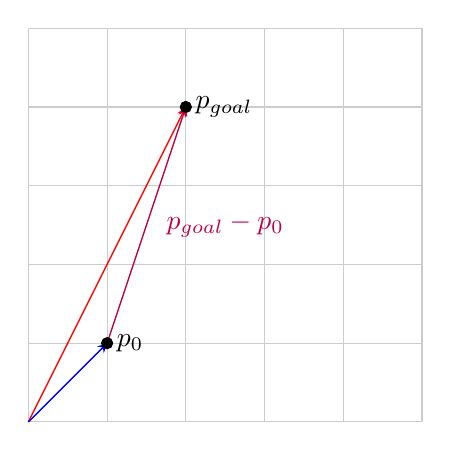
\begin{tikzpicture}
        \draw[thin,gray!40] (0,0) grid (5,5);
        % \draw[<->] (-8,0)--(2,0) node[right]{$x$};
        % \draw[<->] (0,-2)--(0,2) node[above]{$y$};
        % \draw[line width=2pt,blue,-stealth](0,0)--(1,1) node[anchor=south west]{$u$};
        \draw[line width=0.5pt,red,-stealth](0,0)--(2,4) node[anchor=north east]{};
        \draw[line width=0.5pt,blue,-stealth](0,0)--(1,1) node[anchor=north east]{};
        \draw[line width=0.5pt,purple,-stealth](1,1)--(2,4) node at (2.5,2.5){$p_{goal}-p_0$};
        \filldraw[black] (2,4) circle (2pt) node[anchor=west]{$p_{goal}$};
        \filldraw[black] (1,1) circle (2pt) node[anchor=west]{$p_{0}$};
      \end{tikzpicture}
    \caption{2D Coordinate Grid with $p_{goal}$ and $p_{0}$}
    \label{fig:2d-coords}
\end{figure}

Once the agent has determined the transformation vector, $v_g$, it must then determine the optimal combination of pitch and roll commands to reach the goal position. Whilst $v_g$ represents the direction the agent must move in, the components of $v_g$ represent the movement along the global axes, not the agent's local axes. Specifically, the agent's pitch and roll commands will not cause a movement along the global axes, except in the trivial case where the agent is lined up with the global axes.

As such, a change of basis is required to convert the global vector $v_g$ into the local frame of the agent. This change of basis between two vectors represents a linear map between the two vector spaces. More specifically, it represents a linear transformation which maps the global vector $v_g$ to the local vector $v_l$. This transformation is represented by a transformation matrix, $M_2$, such that:

\begin{equation}
    \begin{bmatrix}
    x_l \\
    y_l
    \end{bmatrix}
    = M_2 \cdot
    \begin{bmatrix}
    x_g \\
    y_g
    \end{bmatrix}
\label{eq:basis-transformation2}
\end{equation}

We note that the transformation matrix $M_2$ need only represent the rotation of the agent, as the representations are position and scale invariant; the agent's position and scale do not change between reference frames. In two dimensions, we can extend this simplification as the agent only has the freedom of rotation about a singular axis. Hence, $M_2$ need only be a rotation matrix representing the yaw of the agent.

We can derive $M_2$ by first considering a vector in the global frame, $v_g$ and the local frame $v_l$. We note the vectors have equal magnitudes due to the scale invariance property, thus, it holds that $|v_g| = |v_l|$. We can then determine the angle between the two vectors, $\beta$, and the angle between the global x-axis and the vector $v_g$, $\alpha$, as shown in Fig. \ref{fig:2d-rotation}.

\begin{figure}[ht]
    \centering
    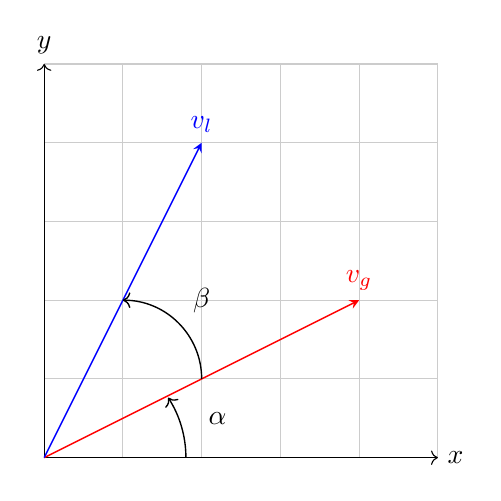
\begin{tikzpicture}
        \draw[thin,gray!40] (0,0) grid (5,5);
        \draw[->] (0,0)--(5,0) node[right]{$x$};
        \draw[->] (0,0)--(0,5) node[above]{$y$};
        % \draw[line width=2pt,blue,-stealth](0,0)--(1,1) node[anchor=south west]{$u$};
        \draw[line width=0.5pt,red,-stealth](0,0)--(4,2) node[above]{$v_g$};
        \draw[line width=0.5pt,blue,-stealth](0,0)--(2,4) node[above]{$v_l$};
        \draw[->,line width=0.5pt] (2,1) arc [start angle=0, end angle=90, radius=1] node at (2,2) {$\beta$};
        \draw[->,line width=0.5pt] (1.8,0) arc [start angle=0, end angle=33, radius=1.4] node at (2.2,0.5) {$\alpha$};
      \end{tikzpicture}
    \caption{2D Coordinate Grid with $v_l$ and $v_g$}
    \label{fig:2d-rotation}
\end{figure}

Thus, we can determine that the $x$ and $y$ components of $v_g$ are:

\begin{equation}
    \begin{aligned}
        x_g &= |v_g| \cos(\alpha) \\
        y_g &= |v_g| \sin(\alpha)
    \end{aligned}
\end{equation}

It must then hold that:

\begin{equation}
    \begin{aligned}
        x_l &= |v_l| \cos(\alpha + \beta) \\
        y_l &= |v_l| \sin(\alpha + \beta) \\
            &\implies \\
        x_l &= |v_g| \cos(\alpha)\cos(\beta) - |v_g| \sin(\alpha)\sin(\beta) \\
        y_l &= |v_g| \sin(\alpha)\cos(\beta) + |v_g| \cos(\alpha)\sin(\beta)
        \\
            &\implies \\
        x_l &= x_g \cos(\beta) - y_g \sin(\beta) \\
        y_l &= x_g \sin(\beta) + y_g \cos(\beta)
    \end{aligned}
\end{equation}

We can represent this as a matrix equation:
\begin{equation}
    \begin{bmatrix}
    x_l \\
    y_l
    \end{bmatrix}
    = 
    \begin{bmatrix}
    \cos(\beta) & -\sin(\beta) \\
    \sin(\beta) & \cos(\beta)
    \end{bmatrix}
    \begin{bmatrix}
    x_g \\
    y_g
    \end{bmatrix}
    \\ \text{, where } \\
    M_2 = 
    \begin{bmatrix}
    \cos(\beta) & -\sin(\beta) \\
    \sin(\beta) & \cos(\beta)
    \end{bmatrix}
\end{equation}

Returning to three dimensions to consider the full movement of the agent, we can extend this method to determine the optimal combination of pitch and roll commands to reach the goal position. We can then determine the transformation matrix $M_3$ to convert the global vector $v_g$ to the local vector $v_l$, such that:

\begin{equation}
   \begin{bmatrix}
    x_l \\
    y_l \\
    z_l
    \end{bmatrix}
    = M_3 \cdot
    \begin{bmatrix}
    x_g \\
    y_g \\
    z_g
    \end{bmatrix}
\label{eq:basis-transformation}
\end{equation}

In the three-dimensional case, $M_3$ will be a rotation matrix representing the yaw, pitch and roll of the agent; we note it is still scale invariant and position invariant. As such, it should be comprised of three individual rotation matrices for each axis of rotation. Hence:

\begin{equation}
    M_3 = R_y \cdot R_x \cdot R_z
\end{equation}

We can then derive each rotation matrix in a similar method to $M_2$. We will consider the rotation about the x-axis first.

We note that $R_x$ will represent a rotation about the x-axis, namely, the roll of the agent. This means that the $y$ and $z$ components of the vector $v_g$ will be rotated through an angle of $\psi$, whilst the $x$ component will remain constant. We can then determine the rotation matrix from earlier intuition:

\begin{equation}
    R_x =
    \begin{bmatrix}
        1 & 0 & 0 \\
        0 & \cos(\psi) & -\sin(\psi) \\
        0 & \sin(\psi) & \cos(\psi)
    \end{bmatrix}
\end{equation}

Considering the other two rotation matrices, $R_y$ and $R_z$, where the $xz$ and $xy$ planes are rotated respectively, we can see:

\begin{equation}
    \begin{aligned}
        R_y &=
        \begin{bmatrix}
        \cos(\theta) & 0 & -\sin(\theta) \\
        0 & 1 & 0 \\
        \sin(\theta) & 0 & \cos(\theta)
        \end{bmatrix}
        \\
        R_z &=
        \begin{bmatrix}
        \cos(\phi) & \sin(\phi) & 0 \\
        -\sin(\phi) & \cos(\phi) & 0 \\
        0 & 0 & 1
        \end{bmatrix} 
    \end{aligned}
\end{equation}

At this stage, we have obtained the transformation matrix $M_3$ to convert the global vector $v_g$ to the local vector $v_l$. We can then determine the optimal combination of pitch and roll commands to reach the goal position, which will be the $x$ and $z$ components of $v_l$ respectively. This is shown in Fig. \ref{fig:pitch-roll}.

\begin{figure}[ht]
    \centering
    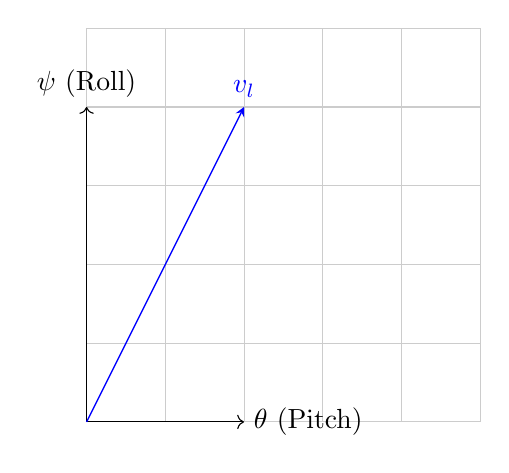
\begin{tikzpicture}
        \draw[thin,gray!40] (0,0) grid (5,5);
        \draw[->] (0,0)--(2,0) node[right]{$\theta$ (Pitch)};
        \draw[->] (0,0)--(0,4) node[above]{$\psi$ (Roll)};
        % \draw[line width=2pt,blue,-stealth](0,0)--(1,1) node[anchor=south west]{$u$};
        % \draw[line width=0.5pt,red,-stealth](0,0)--(4,2) node[above]{$v_g$};
        \draw[line width=0.5pt,blue,-stealth](0,0)--(2,4) node[above]{$v_l$};
        % \draw[->,line width=0.5pt] (2,1) arc [start angle=0, end angle=90, radius=1] node at (2,2) {$\beta$};
        % \draw[->,line width=0.5pt] (1.8,0) arc [start angle=0, end angle=33, radius=1.4] node at (2.2,0.5) {$\alpha$};
      \end{tikzpicture}
    \caption{Constituent Pitch and Roll Components of $v_l$}
    \label{fig:pitch-roll}
\end{figure}

Usefully, this conversion step can be performed in the Unity physics engine using the built-in method \verb|transform.InverseTransformVector()|, which will convert the vector from the global frame to the local frame of the agent. This method is the inverse of the \verb|transform.TransformVector()| method, which converts the vector from the local frame to the global frame.

\subsection{Boids (1987)}
We may now introduce multiple agents into the environment. To reduce the complexity of the position control of the agents, we will assume the agents hover by default. Specifically, when given no control input, the agents resort to a default hover state.

We will make some assumptions about the awareness of the agents at this stage and provide some important definitions.
These are:
\begin{itemize}
    \item Agents are aware of the positions of all other agents within a certain radius, $r$. This is defined as the \emph{neighbourhood radius}.
    \item Agents are aware of their position with respect to the global reference frame.
    \item Agents in a flock of size $n$ are defined as $a_1,...,a_n \in A$.
\end{itemize}

The motivation behind the use of the neighbourhood radius is to reduce computational complexity. Generally, an increase in the number of adjacent agents will increase the number of calculations required. We can reduce this by discounting the agents that have no effect on the behaviour of the agent in question.

We will then introduce the concept of \emph{Boids} \cite{Reynolds}. This is a method of simulating flock behaviour, where agents are programmed to exhibit a set of behaviours that result in emergent flock behaviour. We will explore the implementation of these behaviours in the next section. For all of the following behaviours, we calculate a force vector that is applied to the agent, concerning the agent's local frame.

\subsubsection{Avoidance}

The avoidance behaviour is used as a method for agents to avoid collisions with each other. To this end, the behaviour causes agents to move away from each other when they are within a certain distance of each other. 

We will call this distance $d$, and define it as the \emph{square avoidance radius}. This is the distance at which agents will begin to move away from each other. We will define this as the square of the distance between two agents, $a_1,a_2 \in A$, such that $d = (|a_1|-|a_2|)^2$, for the purposes of algorithmic efficiency. This is a common method in the \emph{Unity} physics engine \cite{unity}.

We can then determine the avoidance vector for an agent, $a$, by calculating the mean distance vector between $a$ and all other agents within the neighbourhood, $a_i$, such that $|a_i| - |a| < d$. Specifically, we populate the set $R_a$ with all agents $a \in A$ that are within the neighbourhood of $a$.

\begin{equation}
\vec{A} = 
\begin{cases}
    0 & \text{if } R_a = \emptyset \\
    \frac{1}{|R_a|} \sum_{a_i \in R_a} \vec{a_i} - \vec{a} & \text{otherwise}
\end{cases}
\end{equation}

We can model an example with two agents in two-dimensional space. This can be seen in Fig. \ref{fig:avoidance-2d}. We see the two agents $a_1$ and $a_2$ have position vectors $[2,2]$ and $[3,3]$ respectively. Hence, the avoidance vectors for the two agents are:

\begin{equation}
    \begin{aligned}
        \vec{a_{avoid}^1} &= \frac{1}{1} \left( \begin{bmatrix} 3 \\ 3 \end{bmatrix} - \begin{bmatrix} 2 \\ 2 \end{bmatrix} \right) = \begin{bmatrix} 1 \\ 1 \end{bmatrix} \\
        \vec{a_{avoid}^2} &= \frac{1}{1} \left( \begin{bmatrix} 2 \\ 2 \end{bmatrix} - \begin{bmatrix} 3 \\ 3 \end{bmatrix} \right) = \begin{bmatrix} -1 \\ -1 \end{bmatrix}
    \end{aligned}
\end{equation}

\begin{figure}[ht]
    \centering
    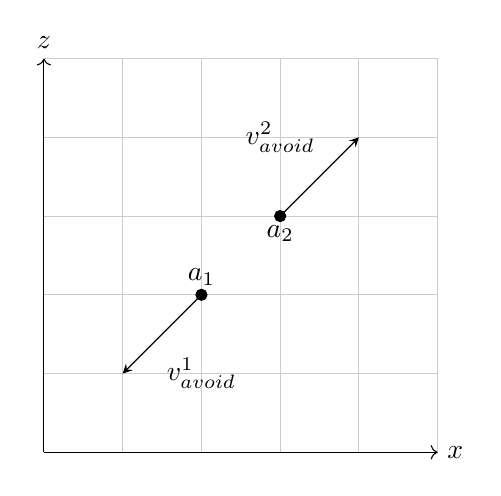
\begin{tikzpicture}
        \draw[thin,gray!40] (0,0) grid (5,5);
        \draw[->] (0,0)--(5,0) node[right]{$x$};
        \draw[->] (0,0)--(0,5) node[above]{$z$};

        \filldraw[black] (2,2) circle (2pt) node[anchor=south]{$a_1$};
        \filldraw[black] (3,3) circle (2pt) node[anchor=north]{$a_2$};

        \draw[line width=0.5pt,black,-stealth](2,2)--(1,1) node at (2,1){$v_{avoid}^1$};
        \draw[line width=0.5pt,black,-stealth](3,3)--(4,4) node at (3,4){$v_{avoid}^2$};
        
      \end{tikzpicture}
    \caption{Avoidance vectors for two nearby agents}
    \label{fig:avoidance-2d}
\end{figure}


\subsubsection{Alignment}

The alignment behaviour causes agents to align their headings with those of their neighbours. This may, in turn, reduce collisions. We can determine the alignment vector for an agent, $a$, by calculating the mean heading vector between $a$ and all other agents within the neighbourhood, $a_i$, such that $|a_i| - |a| < r$. Specifically, we have:

\begin{equation}
\vec{B} =
\begin{cases}
    0 & \text{if } R_b = \emptyset \\
    \frac{1}{|R_b|} \sum_{a_i \in R_b} \vec{h(a_i)} & \text{otherwise}
\end{cases}
\end{equation}

We can model three agents in two-dimensional space. This can be seen in Fig. \ref{fig:alignment-2d}. We see the three agents $a_1$, $a_2$ and $a_3$ have heading vectors $[1,1]$, $[1,0]$ and $[0,1]$ respectively. We introduce three agents as the simplest stable state of the system. Using only two agents would result in a system where the heading vectors would oscillate between the two agents without any external forces. We can then determine the alignment vectors for the three agents as follows:

\begin{equation}
    \begin{aligned}
        \vec{a_{align}^1} &= \frac{1}{2} \left( \begin{bmatrix} 1 \\ 0 \end{bmatrix} + \begin{bmatrix} 0 \\ 1 \end{bmatrix} \right) = \begin{bmatrix} 0.5 \\ 0.5 \end{bmatrix} \\
        \vec{a_{align}^2} &= \frac{1}{2} \left( \begin{bmatrix} 1 \\ 1 \end{bmatrix} + \begin{bmatrix} 0 \\ 1 \end{bmatrix} \right) = \begin{bmatrix} 0.5 \\ 1 \end{bmatrix} \\
        \vec{a_{align}^3} &= \frac{1}{2} \left( \begin{bmatrix} 1 \\ 1 \end{bmatrix} + \begin{bmatrix} 1 \\ 0 \end{bmatrix} \right) = \begin{bmatrix} 1 \\ 0.5 \end{bmatrix}
    \end{aligned}
\end{equation}

We can visualise the current heading vectors at time $t$ and the determined heading vectors for time $t+1$ (indicated in red) in Fig. \ref{fig:alignment-2d}\footnote{N.B. The agents will likely not be in the same position after one timestep. We consider this as negligible in the visualisation.}, where we see the new heading vectors have less variance in their angles.

\begin{figure}[ht]
    \centering
    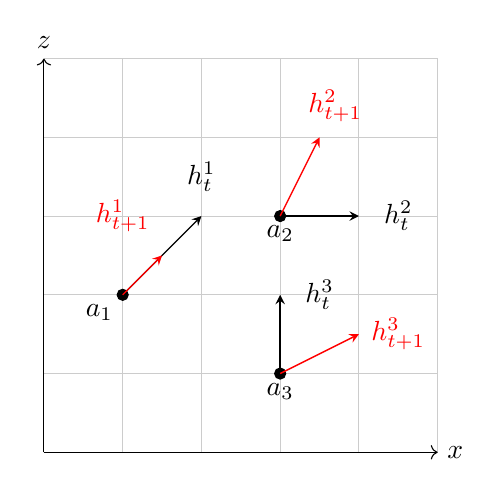
\begin{tikzpicture}
        \draw[thin,gray!40] (0,0) grid (5,5);
        \draw[->] (0,0)--(5,0) node[right]{$x$};
        \draw[->] (0,0)--(0,5) node[above]{$z$};

        \filldraw[black] (1,2) circle (2pt) node[anchor=north east]{$a_1$};
        \filldraw[black] (3,3) circle (2pt) node[anchor=north]{$a_2$};
        \filldraw[black] (3,1) circle (2pt) node[anchor=north]{$a_3$};

        \draw[line width=0.5pt,black,-stealth](1,2)--(2,3) node at (2,3.5){$h^1_t$};
        \draw[line width=0.5pt,black,-stealth](3,3)--(4,3) node at (4.5,3){$h^2_t$};
        \draw[line width=0.5pt,black,-stealth](3,1)--(3,2) node at (3.5,2){$h^3_t$};

        \draw[line width=0.5pt,red,-stealth](1,2)--(1.5,2.5) node at (1,3){$h^1_{t+1}$};
        \draw[line width=0.5pt,red,-stealth](3,3)--(3.5,4) node at (3.7,4.4){$h^2_{t+1}$};
        \draw[line width=0.5pt,red,-stealth](3,1)--(4,1.5) node at (4.5,1.5){$h^3_{t+1}$};
        
      \end{tikzpicture}
    \caption{Alignment vectors for three nearby agents}
    \label{fig:alignment-2d}
\end{figure}


\subsubsection{Cohesion}

Finally, we implement the third principle, \emph{cohesion}. This is in principle, the inverse to the avoidance principle. It ensures members of the flock stay together. We can determine the cohesion vector for an agent, $a$, by calculating the mean position vector between $a$ and all other agents within the neighbourhood, $a_i$, such that $|a_i| - |a| < r$. Specifically, we have:

\begin{equation}
\vec{C} =
\begin{cases}
    0 & \text{if } R_c = \emptyset \\
    \left(
    \frac{1}{|R_c|} \sum_{a_i \in R_c} \vec{a_i} \right) - \vec{a} & \text{otherwise}
\end{cases}
\end{equation}

We consider three agents $a_1$, $a_2$ and $a_3$ in two-dimensional space with position vectors $[1,2]$, $[3,3]$ and $[3,1]$ respectively. We can then determine the cohesion vectors for the three agents as follows:

\begin{equation}
    \begin{aligned}
        \vec{a_{cohere}^1} &= \frac{1}{2} \left( \begin{bmatrix} 3 \\ 3 \end{bmatrix} + \begin{bmatrix} 3 \\ 1 \end{bmatrix} \right) - \begin{bmatrix} 1 \\ 2 \end{bmatrix} = \begin{bmatrix} 2 \\ 0 \end{bmatrix}
        \\
        \vec{a_{cohere}^2} &= \frac{1}{2} \left( \begin{bmatrix} 1 \\ 2 \end{bmatrix} + \begin{bmatrix} 3 \\ 1 \end{bmatrix} \right) - \begin{bmatrix} 3 \\ 3 \end{bmatrix} = \begin{bmatrix} -1 \\ -1.5 \end{bmatrix}
        \\
        \vec{a_{cohere}^3} &= \frac{1}{2} \left( \begin{bmatrix} 1 \\ 2 \end{bmatrix} + \begin{bmatrix} 3 \\ 3 \end{bmatrix} \right) - \begin{bmatrix} 3 \\ 1 \end{bmatrix} = \begin{bmatrix} -1 \\ 1.5 \end{bmatrix}
    \end{aligned}
\end{equation}

Modelling the two agents, we can see the effect of cohesion on the determined cohesion vectors in Fig. \ref{fig:cohesion-2d}. 

\begin{figure}[ht]
    \centering
    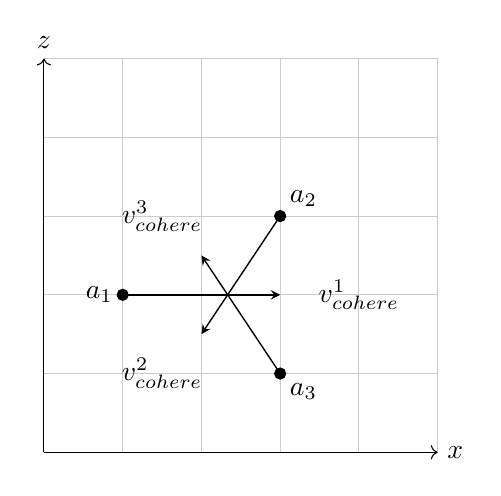
\begin{tikzpicture}
        \draw[thin,gray!40] (0,0) grid (5,5);
        \draw[->] (0,0)--(5,0) node[right]{$x$};
        \draw[->] (0,0)--(0,5) node[above]{$z$};

        \filldraw[black] (1,2) circle (2pt) node[anchor=east]{$a_1$};
        \filldraw[black] (3,3) circle (2pt) node[anchor=south west]{$a_2$};
        \filldraw[black] (3,1) circle (2pt) node[anchor=north west]{$a_3$};

        \draw[line width=0.5pt,black,-stealth](1,2)--(3,2) node at (4,2){$v^1_{cohere}$};
        \draw[line width=0.5pt,black,-stealth](3,3)--(2,1.5) node at (1.5,1){$v^2_{cohere}$};
        \draw[line width=0.5pt,black,-stealth](3,1)--(2,2.5) node at (1.5,3){$v^3_{cohere}$};
        
      \end{tikzpicture}
    \caption{Alignment vectors for three nearby agents}
    \label{fig:cohesion-2d}
\end{figure}

\subsubsection{Combining Behaviours}
\label{sec:combining-behaviours}

Fig. \ref{fig:cohesion-2d} demonstrates that the balance between cohesion and separation is important. If the cohesion force is too strong, the agents will collide, as shown. If the separation force is too strong, the agents will become disconnected and fly apart. This is similar in principle to the \emph{strong nuclear force} acting within the nucleus of an atom. The force is repulsive at close ranges (the avoidance radius), but attractive at larger ranges (the neighbourhood). We will explore this further in Section \ref{sec:lpfe}.

In general, tuning the influence of all three components is challenging. Even considering the constants in the simulation, \citet{Reynolds} notes that the relative weights that influence the strength of each component `\emph{is a precarious interrelationship that is difficult to adjust}'. Despite this, we can combine these three independent behaviours and attempt to tune them. 

We can define a \emph{composite behaviour}, which is defined as a linear combination of weights and behaviour vectors. In three dimensions, for the three behaviours, we have:

\begin{equation}
    \vec{V} = \alpha
    \begin{bmatrix}
    x_{avoid} \\
    y_{avoid} \\
    z_{avoid}
    \end{bmatrix}
    +
    \beta
    \begin{bmatrix}
    x_{align} \\
    y_{align} \\
    z_{align}
    \end{bmatrix}
    +
    \gamma
    \begin{bmatrix}
    x_{cohere} \\
    y_{cohere} \\
    z_{cohere}
    \end{bmatrix}
\end{equation}

We will utilise an empirical method for tuning the constants $\alpha, \beta$ and $\gamma$. We will simulate the agents in a controlled environment and adjust the constants until the agents exhibit appropriate emergent flock behaviour. We will then analyse the emergent behaviour and adjust the constants accordingly.

Initially, we will set the constants as shown in Table \ref{tab:spawn-constants}. Additionally, we will set the weights to be equal for each component as shown in Table \ref{tab:boids-weights}.

\begin{table}[ht]
    \begin{minipage}{0.45\textwidth}
        \centering
        \begin{tabular}{| c | c |} 
        \hline
        Constant & Value \\ 
        \hline\hline
        Number of Agents & 8 \\
        \hline
        Spawn Radius & 4 \\
        \hline
        Neighbour Radius & 1 \\
        \hline
        Square Avoidance Radius & 16 \\
        \hline
        \end{tabular}
        \caption{Spawn Constants}
        \label{tab:spawn-constants}
    \end{minipage}
    \hfill
    \begin{minipage}{0.45\textwidth}
        \centering
        \begin{tabular}{| c | c |} 
        \hline
        Behaviour & Weight \\ 
        \hline\hline
        Separation & 1 \\
        \hline
        Alignment & 1 \\
        \hline
        Cohesion & 1 \\
        \hline
        \end{tabular}
        \caption{Boids Weights}
        \label{tab:boids-weights}
    \end{minipage}
\end{table}

Figure \ref{fig:exp1} shows the x-z positions of the agents within the flock over a simulated run with these constants. We see that the agents move together in a straight line, signifying that the alignment weight is initially well-tuned. 

We note that the behaviour of some agents is not as is desired, as in Fig. \ref{fig:exp1}, we see there exists a large gap between two agents. This is likely due to the avoidance weight being too low, causing the agents to not move closer to each other. As a result, we will increase the avoidance weight to \textbf{1.5} and re-run the simulation. We will also increase the neighbourhood radius to \textbf{3} to mitigate issues with agents not being aware of each other.


\begin{figure}[ht]
\centering
\begin{subfigure}{.4\textwidth}
\begin{tikzpicture}[trim axis left, trim axis right]
    \begin{axis}[
        xlabel=X,
        ylabel=Z,
        legend pos=outer north east,
        colormap/cool,
    ]

    \draw (axis cs:0,0) circle [blue, radius=4];


\addplot [scatter, surf, mark=*, x filter/.code={\IfStrEq{\thisrow{DroneID}}{Agent 0}{}{\def\pgfmathresult{}}{\def\pgfmathresult{}}},]
    table [x=X, y=Z, col sep=comma, point meta=\thisrow{Time}] {droneData.csv};

\addplot [scatter, surf, mark=*, x filter/.code={\IfStrEq{\thisrow{DroneID}}{Agent 1}{}{\def\pgfmathresult{}}{\def\pgfmathresult{}}},]
    table [x=X, y=Z, col sep=comma, point meta=\thisrow{Time}] {droneData.csv};

\addplot [scatter, surf, mark=*, x filter/.code={\IfStrEq{\thisrow{DroneID}}{Agent 2}{}{\def\pgfmathresult{}}{\def\pgfmathresult{}}},]
    table [x=X, y=Z, col sep=comma, point meta=\thisrow{Time}] {droneData.csv};

\addplot [scatter, surf, mark=*, x filter/.code={\IfStrEq{\thisrow{DroneID}}{Agent 3}{}{\def\pgfmathresult{}}{\def\pgfmathresult{}}},]
    table [x=X, y=Z, col sep=comma, point meta=\thisrow{Time}] {droneData.csv};

\addplot [scatter, surf, mark=*, x filter/.code={\IfStrEq{\thisrow{DroneID}}{Agent 4}{}{\def\pgfmathresult{}}{\def\pgfmathresult{}}},]
    table [x=X, y=Z, col sep=comma, point meta=\thisrow{Time}] {droneData.csv};

\addplot [scatter, surf, mark=*, x filter/.code={\IfStrEq{\thisrow{DroneID}}{Agent 5}{}{\def\pgfmathresult{}}{\def\pgfmathresult{}}},]
    table [x=X, y=Z, col sep=comma, point meta=\thisrow{Time}] {droneData.csv};

\addplot [scatter, surf, mark=*, x filter/.code={\IfStrEq{\thisrow{DroneID}}{Agent 6}{}{\def\pgfmathresult{}}{\def\pgfmathresult{}}},]
    table [x=X, y=Z, col sep=comma, point meta=\thisrow{Time}] {droneData.csv};

\addplot [scatter, surf, mark=*, x filter/.code={\IfStrEq{\thisrow{DroneID}}{Agent 7}{}{\def\pgfmathresult{}}{\def\pgfmathresult{}}},]
    table [x=X, y=Z, col sep=comma, point meta=\thisrow{Time}] {droneData.csv};
    
    \end{axis}
\end{tikzpicture}
\caption{Initial}
\label{fig:exp1}
\end{subfigure}
\hfill
\begin{subfigure}{.4\textwidth}
    \begin{tikzpicture}[trim axis left, trim axis right]
        \begin{axis}[
            xlabel=X,
            ylabel=Z,
            legend pos=outer north east,
            colormap/cool,
        ]
    
        \draw (axis cs:0,0) circle [blue, radius=4];
    
    
    \addplot [scatter, surf, mark=*, x filter/.code={\IfStrEq{\thisrow{DroneID}}{Agent 0}{}{\def\pgfmathresult{}}{\def\pgfmathresult{}}},]
        table [x=X, y=Z, col sep=comma, point meta=\thisrow{Time}] {drone2.csv};
    
    \addplot [scatter, surf, mark=*, x filter/.code={\IfStrEq{\thisrow{DroneID}}{Agent 1}{}{\def\pgfmathresult{}}{\def\pgfmathresult{}}},]
        table [x=X, y=Z, col sep=comma, point meta=\thisrow{Time}] {drone2.csv};
    
    \addplot [scatter, surf, mark=*, x filter/.code={\IfStrEq{\thisrow{DroneID}}{Agent 2}{}{\def\pgfmathresult{}}{\def\pgfmathresult{}}},]
        table [x=X, y=Z, col sep=comma, point meta=\thisrow{Time}] {drone2.csv};
    
    \addplot [scatter, surf, mark=*, x filter/.code={\IfStrEq{\thisrow{DroneID}}{Agent 3}{}{\def\pgfmathresult{}}{\def\pgfmathresult{}}},]
        table [x=X, y=Z, col sep=comma, point meta=\thisrow{Time}] {drone2.csv};
    
    \addplot [scatter, surf, mark=*, x filter/.code={\IfStrEq{\thisrow{DroneID}}{Agent 4}{}{\def\pgfmathresult{}}{\def\pgfmathresult{}}},]
        table [x=X, y=Z, col sep=comma, point meta=\thisrow{Time}] {drone2.csv};
    
    \addplot [scatter, surf, mark=*, x filter/.code={\IfStrEq{\thisrow{DroneID}}{Agent 5}{}{\def\pgfmathresult{}}{\def\pgfmathresult{}}},]
        table [x=X, y=Z, col sep=comma, point meta=\thisrow{Time}] {drone2.csv};
    
    \addplot [scatter, surf, mark=*, x filter/.code={\IfStrEq{\thisrow{DroneID}}{Agent 6}{}{\def\pgfmathresult{}}{\def\pgfmathresult{}}},]
        table [x=X, y=Z, col sep=comma, point meta=\thisrow{Time}] {drone2.csv};
    
    \addplot [scatter, surf, mark=*, x filter/.code={\IfStrEq{\thisrow{DroneID}}{Agent 7}{}{\def\pgfmathresult{}}{\def\pgfmathresult{}}},]
        table [x=X, y=Z, col sep=comma, point meta=\thisrow{Time}] {drone2.csv};
        
        \end{axis}
    \end{tikzpicture}
    \caption{Avoidance Tuning}
    \label{fig:exp2}
\end{subfigure}
\caption{Simulation Run (Start is indicated by black circle)} 
\end{figure}

The results of the simulation with the updated values are shown in Fig. \ref{fig:exp2}. We note that the agents initially move away from each other due to the increased effects of avoidance, however, the leftmost two agents appear to not be pulled closer together, despite being within each other's neighbourhood. 

To mitigate this, we can increase the weight of cohesion to \textbf{1.4} and reduce the square avoidance radius to \textbf{12}. Finally, we can increase the weight of alignment slightly, to \textbf{1.2}, to reduce the effects of agents veering at the sides of the flock. This simulation results in the positions in Fig. \ref{fig:exp3}.

\begin{figure}[ht]
    \centering
    \begin{tikzpicture}[trim axis left, trim axis right]
        \begin{axis}[
            xlabel=X,
            ylabel=Z,
            legend pos=outer north east,
            colormap/cool,
        ]
    
        \draw (axis cs:0,0) circle [blue, radius=4];
    
    
    \addplot [scatter, surf, mark=*, x filter/.code={\IfStrEq{\thisrow{DroneID}}{Agent 0}{}{\def\pgfmathresult{}}{\def\pgfmathresult{}}},]
        table [x=X, y=Z, col sep=comma, point meta=\thisrow{Time}] {drone3.csv};
    
    \addplot [scatter, surf, mark=*, x filter/.code={\IfStrEq{\thisrow{DroneID}}{Agent 1}{}{\def\pgfmathresult{}}{\def\pgfmathresult{}}},]
        table [x=X, y=Z, col sep=comma, point meta=\thisrow{Time}] {drone3.csv};
    
    \addplot [scatter, surf, mark=*, x filter/.code={\IfStrEq{\thisrow{DroneID}}{Agent 2}{}{\def\pgfmathresult{}}{\def\pgfmathresult{}}},]
        table [x=X, y=Z, col sep=comma, point meta=\thisrow{Time}] {drone3.csv};
    
    \addplot [scatter, surf, mark=*, x filter/.code={\IfStrEq{\thisrow{DroneID}}{Agent 3}{}{\def\pgfmathresult{}}{\def\pgfmathresult{}}},]
        table [x=X, y=Z, col sep=comma, point meta=\thisrow{Time}] {drone3.csv};
    
    \addplot [scatter, surf, mark=*, x filter/.code={\IfStrEq{\thisrow{DroneID}}{Agent 4}{}{\def\pgfmathresult{}}{\def\pgfmathresult{}}},]
        table [x=X, y=Z, col sep=comma, point meta=\thisrow{Time}] {drone3.csv};
    
    \addplot [scatter, surf, mark=*, x filter/.code={\IfStrEq{\thisrow{DroneID}}{Agent 5}{}{\def\pgfmathresult{}}{\def\pgfmathresult{}}},]
        table [x=X, y=Z, col sep=comma, point meta=\thisrow{Time}] {drone3.csv};
    
    \addplot [scatter, surf, mark=*, x filter/.code={\IfStrEq{\thisrow{DroneID}}{Agent 6}{}{\def\pgfmathresult{}}{\def\pgfmathresult{}}},]
        table [x=X, y=Z, col sep=comma, point meta=\thisrow{Time}] {drone3.csv};
    
    \addplot [scatter, surf, mark=*, x filter/.code={\IfStrEq{\thisrow{DroneID}}{Agent 7}{}{\def\pgfmathresult{}}{\def\pgfmathresult{}}},]
        table [x=X, y=Z, col sep=comma, point meta=\thisrow{Time}] {drone3.csv};
        
        \end{axis}
    \end{tikzpicture}
    \caption{Final Tuning}
    \label{fig:exp3}
\end{figure}

We note that the agents now move together in a cohesive manner and are responsive to each other's movements. However, the flock's movement is not perfect; the agents have a tendency to spread apart and occasionally overcorrect, causing collisions and erratic behaviour. At this stage, we have obtained a reasonable balance between the three behaviours, with the final constants shown in Table \ref{tab:boids-weights-final}.

\begin{table}[ht]
    \centering
    \begin{tabular}{| c | c |} 
    \hline
    Behaviour & Weight \\ 
    \hline\hline
    Separation & 1.5 \\
    \hline
    Alignment & 1.2 \\
    \hline
    Cohesion & 1.4 \\
    \hline
    \end{tabular}
    \caption{Final Boids Weights}
    \label{tab:boids-weights-final}
\end{table}

We have demonstrated the difficulty in tuning the parameters for the Boids algorithm using an empirical method. In a similar fashion to the exploration of tuning the PID controller in Section \ref{sec:pid-tuning}, we will explore heuristic methods to tune the parameters of the Boids algorithm at a later stage.

\subsection{Extended Boids}
We have implemented the three fundamental behaviours of the Boids algorithm. At this stage, we can extend the algorithm to include additional behaviours, allowing us to simulate more complex emergent behaviours and provide a framework for simulating a more life-like environment for the agents.

We will consider two such extensions: \emph{goal-seeking} and \emph{terrain avoidance}. We will implement these behaviours in the simulation and analyse the emergent behaviours of the agents.



\subsubsection{Goal Seeking}
\label{sec:goal-seek}
One key extension to the Boids algorithm is the inclusion of a \emph{goal-seeking} behaviour, which allows the agents to seek a goal position within the world. Specifically, we can implement a variation of a simple pathfinding ability for the agents. The ability for autonomous agents to perform effective path planning plays a key role in autonomous control systems\cite{liu2020autonomous}. 

Whilst in the real world, path planning is a complex problem involving balancing computational complexity and optimality, we can implement a simple pathfinding algorithm for the agents in the simulation by making a key assumption about the environment; that the agents are aware of the goal position.

In reality, the agents would need to be able to sense the environment and determine the goal position. This could be achieved through the use of sensors, such as cameras or LIDAR, or through the use of a global positioning system (GPS)\cite{Petrillo,burwell_2019}.

We can implement the agents' ability to seek a goal position in a similar method to the three behaviours Reynolds mentions. We can define a \emph{goal sphere}, with a given radius, centred around a random position in the world. We can then implement the \emph{seeking} behaviour to calculate the distance vector between the agent and the goal in order to apply a force in the direction of the goal.

Specifically, we have:

\begin{equation}
\vec{D} = \vec{g} - \vec{a}
\end{equation}
    
Where $\vec{D}$ is the distance vector between the agent, $a$, and the goal, $g$.

As with the previous behaviours, we will simulate the agents in a controlled environment and adjust the constants until the agents exhibit appropriate emergent flock behaviour. A run of the simulation with the goal-seeking behaviour weight set at \textbf{2} is shown in Fig. \ref{fig:exp4}\footnote{The location of the goal is shown by the green circle in the figure.}. 

We note that the agents do not actually enter the goal radius, instead orbiting around the goal. This behaviour was likely down to the method being used before to implement the agent's moves; the agent would receive the given force vector, and then normalise it - acting as a maximum clamping value for the force. 

This turned out to not be the best practice, as whilst in close spaces, the direction of the desired goal \emph{(e.g. avoidance of nearby neighbours)} would be more important than the magnitude of the force, at higher distances between the current and goal position of the agent, the magnitudes, specifically of the pitch and roll components, become more significant in path planning. 

As an alternative, we simply use Unity's built-in \verb|Math.Clamp| function, which clamps a value between a minimum and maximum value. This allows us to set the minimum and maximum force values to ones we deem safe.

\begin{figure}[ht]
\centering
\begin{subfigure}{.45\textwidth}
\begin{tikzpicture}[trim axis left, trim axis right]
    \begin{axis}[
        axis equal,
        xlabel=X,
        ylabel=Z,
        legend pos=outer north east,
        colormap/cool,
        width=1.2\textwidth
    ]


    \draw (axis cs:0,0) circle [radius=4];
    


\addplot [scatter, surf, mark=*, x filter/.code={\IfStrEq{\thisrow{DroneID}}{Agent 0}{}{\def\pgfmathresult{}}{\def\pgfmathresult{}}},]
    table [x=X, y=Z, col sep=comma, point meta=\thisrow{Time}] {drone4.csv};

\addplot [scatter, surf, mark=*, x filter/.code={\IfStrEq{\thisrow{DroneID}}{Agent 1}{}{\def\pgfmathresult{}}{\def\pgfmathresult{}}},]
    table [x=X, y=Z, col sep=comma, point meta=\thisrow{Time}] {drone4.csv};

\addplot [scatter, surf, mark=*, x filter/.code={\IfStrEq{\thisrow{DroneID}}{Agent 2}{}{\def\pgfmathresult{}}{\def\pgfmathresult{}}},]
    table [x=X, y=Z, col sep=comma, point meta=\thisrow{Time}] {drone4.csv};

\addplot [scatter, surf, mark=*, x filter/.code={\IfStrEq{\thisrow{DroneID}}{Agent 3}{}{\def\pgfmathresult{}}{\def\pgfmathresult{}}},]
    table [x=X, y=Z, col sep=comma, point meta=\thisrow{Time}] {drone4.csv};

\addplot [scatter, surf, mark=*, x filter/.code={\IfStrEq{\thisrow{DroneID}}{Agent 4}{}{\def\pgfmathresult{}}{\def\pgfmathresult{}}},]
    table [x=X, y=Z, col sep=comma, point meta=\thisrow{Time}] {drone4.csv};

\addplot [scatter, surf, mark=*, x filter/.code={\IfStrEq{\thisrow{DroneID}}{Agent 5}{}{\def\pgfmathresult{}}{\def\pgfmathresult{}}},]
    table [x=X, y=Z, col sep=comma, point meta=\thisrow{Time}] {drone4.csv};

\addplot [scatter, surf, mark=*, x filter/.code={\IfStrEq{\thisrow{DroneID}}{Agent 6}{}{\def\pgfmathresult{}}{\def\pgfmathresult{}}},]
    table [x=X, y=Z, col sep=comma, point meta=\thisrow{Time}] {drone4.csv};

\addplot [scatter, surf, mark=*, x filter/.code={\IfStrEq{\thisrow{DroneID}}{Agent 7}{}{\def\pgfmathresult{}}{\def\pgfmathresult{}}},]
    table [x=X, y=Z, col sep=comma, point meta=\thisrow{Time}] {drone4.csv};

    \draw [green, line width=0.7mm] (axis cs:-16,-29) circle [radius=3.45];
    
    \end{axis}
\end{tikzpicture}
\caption{Normalised Force Vector}
\label{fig:exp4}
\end{subfigure}
\hfill
\begin{subfigure}{.45\textwidth}
    \centering
    \begin{tikzpicture}[trim axis left, trim axis right]
        \begin{axis}[
            axis equal,
            xlabel=X,
            ylabel=Z,
            legend pos=outer north east,
            colormap/cool,
            width=1.2\textwidth
        ]
    
        \draw (axis cs:0,0) circle [radius=4];
    
    
    \addplot [scatter, surf, mark=*, x filter/.code={\IfStrEq{\thisrow{DroneID}}{Agent 0}{}{\def\pgfmathresult{}}{\def\pgfmathresult{}}},]
        table [x=X, y=Z, col sep=comma, point meta=\thisrow{Time}] {drone5.csv};
    
    \addplot [scatter, surf, mark=*, x filter/.code={\IfStrEq{\thisrow{DroneID}}{Agent 1}{}{\def\pgfmathresult{}}{\def\pgfmathresult{}}},]
        table [x=X, y=Z, col sep=comma, point meta=\thisrow{Time}] {drone5.csv};
    
    \addplot [scatter, surf, mark=*, x filter/.code={\IfStrEq{\thisrow{DroneID}}{Agent 2}{}{\def\pgfmathresult{}}{\def\pgfmathresult{}}},]
        table [x=X, y=Z, col sep=comma, point meta=\thisrow{Time}] {drone5.csv};
    
    \addplot [scatter, surf, mark=*, x filter/.code={\IfStrEq{\thisrow{DroneID}}{Agent 3}{}{\def\pgfmathresult{}}{\def\pgfmathresult{}}},]
        table [x=X, y=Z, col sep=comma, point meta=\thisrow{Time}] {drone5.csv};
    
    \addplot [scatter, surf, mark=*, x filter/.code={\IfStrEq{\thisrow{DroneID}}{Agent 4}{}{\def\pgfmathresult{}}{\def\pgfmathresult{}}},]
        table [x=X, y=Z, col sep=comma, point meta=\thisrow{Time}] {drone5.csv};
    
    \addplot [scatter, surf, mark=*, x filter/.code={\IfStrEq{\thisrow{DroneID}}{Agent 5}{}{\def\pgfmathresult{}}{\def\pgfmathresult{}}},]
        table [x=X, y=Z, col sep=comma, point meta=\thisrow{Time}] {drone5.csv};
    
    \addplot [scatter, surf, mark=*, x filter/.code={\IfStrEq{\thisrow{DroneID}}{Agent 6}{}{\def\pgfmathresult{}}{\def\pgfmathresult{}}},]
        table [x=X, y=Z, col sep=comma, point meta=\thisrow{Time}] {drone5.csv};
    
    \addplot [scatter, surf, mark=*, x filter/.code={\IfStrEq{\thisrow{DroneID}}{Agent 7}{}{\def\pgfmathresult{}}{\def\pgfmathresult{}}},]
        table [x=X, y=Z, col sep=comma, point meta=\thisrow{Time}] {drone5.csv};
    
    \draw [green, line width=0.7mm] (axis cs:27,22) circle [radius=3.45];

    \end{axis}
\end{tikzpicture}
\caption{Clamped Force Vector}
\label{fig:exp5}
\end{subfigure}
\caption{Seeking Behaviour}
\label{fig:exp45}
\end{figure}

The behaviour now seen in Fig. \ref{fig:exp5} is accurate, but not ideal, as the agents overshoot the goal and find themselves backtracking during pathfinding. This can be mitigated by implementing an error controller, using the fundamentals of control theory discussed in Section \ref{sec:stabilisation}.

To this extent, we may implement a proportional controller to adjust the force applied to the agents based on the distance between the agent and the goal. Specifically, the determined force is inversely proportional to the distance between the agent and the goal.

We can then instruct the agents to stop once they have detected that they are within the goal space. An example simulation of this is shown in Fig. \ref{fig:exp6}. We note that the agents gravitate towards the centre of the goal space. This is unwanted, as it does not make enough considerations for adjacent agents and their respective avoidance radii. 

At this stage, we can then reintroduce our three initial behaviours and their final values from the empirical tuning in Table \ref{tab:boids-weights-final} and tune the influence of the seeking behaviour accordingly.

\begin{figure}[ht]
    \centering
    \begin{subfigure}{.45\textwidth}
    \begin{tikzpicture}[trim axis left, trim axis right]
        \begin{axis}[
            axis equal,
            xlabel=X,
            ylabel=Z,
            legend pos=outer north east,
            colormap/cool,
            width=1.2\textwidth
        ]
    
        \draw (axis cs:0,0) circle [radius=4];
    
    
    \addplot [scatter, surf, mark=*, x filter/.code={\IfStrEq{\thisrow{DroneID}}{Agent 0}{}{\def\pgfmathresult{}}{\def\pgfmathresult{}}},]
        table [x=X, y=Z, col sep=comma, point meta=\thisrow{Time}] {drone6.csv};
    
    \addplot [scatter, surf, mark=*, x filter/.code={\IfStrEq{\thisrow{DroneID}}{Agent 1}{}{\def\pgfmathresult{}}{\def\pgfmathresult{}}},]
        table [x=X, y=Z, col sep=comma, point meta=\thisrow{Time}] {drone6.csv};
    
    \addplot [scatter, surf, mark=*, x filter/.code={\IfStrEq{\thisrow{DroneID}}{Agent 2}{}{\def\pgfmathresult{}}{\def\pgfmathresult{}}},]
        table [x=X, y=Z, col sep=comma, point meta=\thisrow{Time}] {drone6.csv};
    
    \addplot [scatter, surf, mark=*, x filter/.code={\IfStrEq{\thisrow{DroneID}}{Agent 3}{}{\def\pgfmathresult{}}{\def\pgfmathresult{}}},]
        table [x=X, y=Z, col sep=comma, point meta=\thisrow{Time}] {drone6.csv};
    
    \addplot [scatter, surf, mark=*, x filter/.code={\IfStrEq{\thisrow{DroneID}}{Agent 4}{}{\def\pgfmathresult{}}{\def\pgfmathresult{}}},]
        table [x=X, y=Z, col sep=comma, point meta=\thisrow{Time}] {drone6.csv};
    
    \addplot [scatter, surf, mark=*, x filter/.code={\IfStrEq{\thisrow{DroneID}}{Agent 5}{}{\def\pgfmathresult{}}{\def\pgfmathresult{}}},]
        table [x=X, y=Z, col sep=comma, point meta=\thisrow{Time}] {drone6.csv};
    
    \addplot [scatter, surf, mark=*, x filter/.code={\IfStrEq{\thisrow{DroneID}}{Agent 6}{}{\def\pgfmathresult{}}{\def\pgfmathresult{}}},]
        table [x=X, y=Z, col sep=comma, point meta=\thisrow{Time}] {drone6.csv};
    
    \addplot [scatter, surf, mark=*, x filter/.code={\IfStrEq{\thisrow{DroneID}}{Agent 7}{}{\def\pgfmathresult{}}{\def\pgfmathresult{}}},]
        table [x=X, y=Z, col sep=comma, point meta=\thisrow{Time}] {drone6.csv};
    
    \draw [green, line width=0.7mm] (axis cs:21,-19) circle [radius=3.45];

    \end{axis}
\end{tikzpicture}
\caption{Final Seeking Behaviour}
\label{fig:exp6}
\end{subfigure}
\hfill
\begin{subfigure}{.45\textwidth}
    \centering
    \begin{tikzpicture}[trim axis left, trim axis right]
        \begin{axis}[
            axis equal,
            xlabel=X,
            ylabel=Z,
            legend pos=outer north east,
            colormap/cool,
            width=1.2\textwidth
        ]
    
        \draw (axis cs:0,0) circle [radius=4];
    
    
    \addplot [scatter, surf, mark=*, x filter/.code={\IfStrEq{\thisrow{DroneID}}{Agent 0}{}{\def\pgfmathresult{}}{\def\pgfmathresult{}}},]
        table [x=X, y=Z, col sep=comma, point meta=\thisrow{Time}] {drone7.csv};
    
    \addplot [scatter, surf, mark=*, x filter/.code={\IfStrEq{\thisrow{DroneID}}{Agent 1}{}{\def\pgfmathresult{}}{\def\pgfmathresult{}}},]
        table [x=X, y=Z, col sep=comma, point meta=\thisrow{Time}] {drone7.csv};
    
    \addplot [scatter, surf, mark=*, x filter/.code={\IfStrEq{\thisrow{DroneID}}{Agent 2}{}{\def\pgfmathresult{}}{\def\pgfmathresult{}}},]
        table [x=X, y=Z, col sep=comma, point meta=\thisrow{Time}] {drone7.csv};
    
    \addplot [scatter, surf, mark=*, x filter/.code={\IfStrEq{\thisrow{DroneID}}{Agent 3}{}{\def\pgfmathresult{}}{\def\pgfmathresult{}}},]
        table [x=X, y=Z, col sep=comma, point meta=\thisrow{Time}] {drone7.csv};
    
    \addplot [scatter, surf, mark=*, x filter/.code={\IfStrEq{\thisrow{DroneID}}{Agent 4}{}{\def\pgfmathresult{}}{\def\pgfmathresult{}}},]
        table [x=X, y=Z, col sep=comma, point meta=\thisrow{Time}] {drone7.csv};
    
    \addplot [scatter, surf, mark=*, x filter/.code={\IfStrEq{\thisrow{DroneID}}{Agent 5}{}{\def\pgfmathresult{}}{\def\pgfmathresult{}}},]
        table [x=X, y=Z, col sep=comma, point meta=\thisrow{Time}] {drone7.csv};
    
    \addplot [scatter, surf, mark=*, x filter/.code={\IfStrEq{\thisrow{DroneID}}{Agent 6}{}{\def\pgfmathresult{}}{\def\pgfmathresult{}}},]
        table [x=X, y=Z, col sep=comma, point meta=\thisrow{Time}] {drone7.csv};
    
    \addplot [scatter, surf, mark=*, x filter/.code={\IfStrEq{\thisrow{DroneID}}{Agent 7}{}{\def\pgfmathresult{}}{\def\pgfmathresult{}}},]
        table [x=X, y=Z, col sep=comma, point meta=\thisrow{Time}] {drone7.csv};
    
    \draw [green, line width=0.7mm] (axis cs:-29,12) circle [radius=3.45];

    \end{axis}
\end{tikzpicture}
\caption{Three Initial Behaviours + Seeking}
\label{fig:exp7}
\end{subfigure}
\caption{Finalising Seeking Behaviour}
\label{fig:exp67}
\end{figure}

We note that the agents now exhibit the flocking behaviour present previously, with the additional ability to seek a goal; this causes the agents to move in a cohesive manner towards the goal. It follows that the weight of the seeking behaviour will also need tuning alongside the three initial behaviours. 

\subsubsection{Terrain Generation}
In previous sections, we have focused on the pathfinding behaviour of the agents in empty space. However, in the real world, there are many obstacles that the agents must avoid. Hence, in this section, we introduce a terrain model to the simulation to parallel real-world deviations in terrain heights. 

In this project, we employ Perlin noise\cite[289-293]{Perlin} to create textures that effectively model terrain. This method generates a texture that, when translated into a heightmap, assigns elevations based on color intensity at specific points. The smooth terrain this method produces, thanks to the interpolated noise function, aligns perfectly with our project's goals.

For our simulation, we focus on crafting a waveform characterised by a specific frequency, \(f\), and amplitude, \(A\), to replicate the terrain's undulations. This waveform is crucial in generating our heightmap. We delve into four critical parameters that define our terrain generation process: the number of octaves, \(O_n\); lacunarity, \(l\); persistence, \(p\); and scale, \(s\).

An octave in this context refers to the frequency ratio within a waveform, echoing its musical counterpart by signifying a frequency doubling. The octave count, \(O_n\), indicates how often the waveform's frequency is doubled, offering us a tool to enhance the terrain's detail level. A higher octave count means more nuanced terrain details, catering to the precision our simulation demands.

The effect of the number of octaves on one-dimensional Perlin noise is shown in Fig. \ref{fig:octaves-1d}. We can see that as the number of octaves increases, the detail in the waveform increases. Generalising over multiple dimensions, we can see that the number of octaves controls the level of detail in the terrain.

\begin{figure}[ht]
    \centering
    \begin{subfigure}{0.4\textwidth}
        \centering
        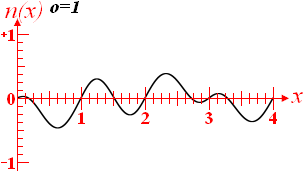
\includegraphics[width=\linewidth]{octave1.png}
        \caption{$O_n=1$}
        \label{fig:octave1}
    \end{subfigure}
    \hfill
    \begin{subfigure}{0.4\textwidth}
        \centering
        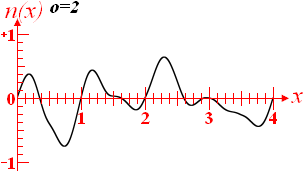
\includegraphics[width=\linewidth]{octave2.png}
        \caption{$O_n=2$}
        \label{fig:octave2}
    \end{subfigure}
    \hfill
    \begin{subfigure}{0.4\textwidth}
        \centering
        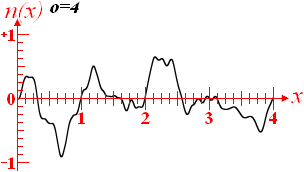
\includegraphics[width=\linewidth]{octave4.png}
        \caption{$O_n=4$}
        \label{fig:octave4}
    \end{subfigure}
    \hfill
    \begin{subfigure}{0.4\textwidth}
        \centering
        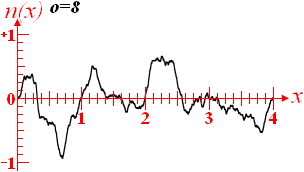
\includegraphics[width=\linewidth]{octave8.png}
        \caption{$O_n=8$}
        \label{fig:octave8}
    \end{subfigure}
    \caption{$O_n$ effect on 1-D Perlin noise\cite{libnoise}}
    \label{fig:octaves-1d}
\end{figure}

Accordingly, the lacunarity, $l$, controls the increase in frequency between octaves; an increase in lacunarity results in an increase in frequency between octaves. This is characterised by the relationship:

$$\forall x \in \{O_1,O_2,...,O_n\}, f_x = l^{O_x}$$

Lacunarity, then, allows us to tune the increase in detail between octaves. We can see in Fig. \ref{fig:lacunarity}, with four octaves, the effect of lacunarity on the generated terrain. We can see that as the lacunarity increases, the terrain becomes more `spiky' due to the increased detail level.

\begin{figure}[ht]
    \centering
    \begin{subfigure}{0.3\textwidth}
        \centering
        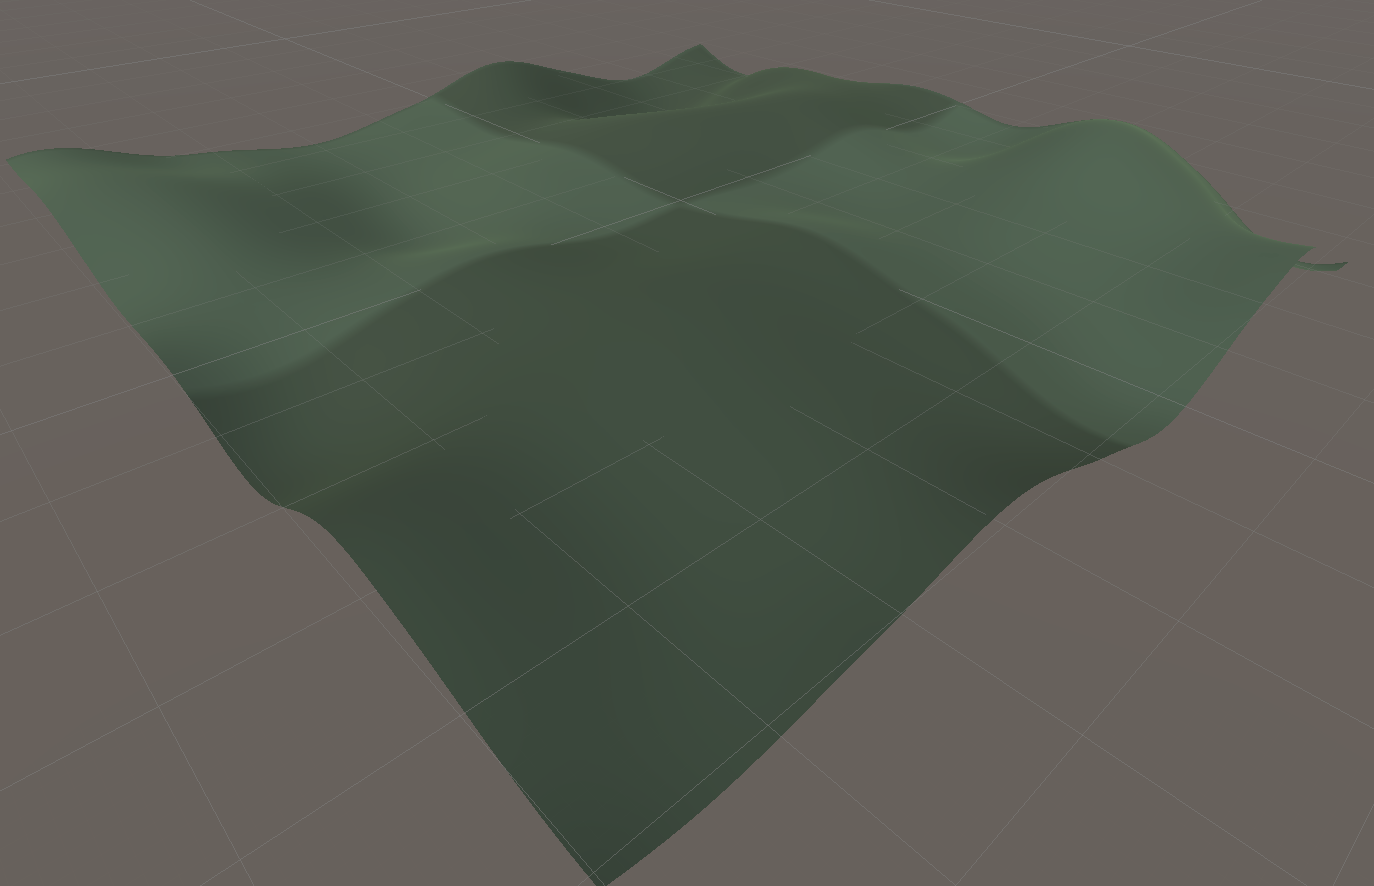
\includegraphics[width=\linewidth]{lacunarity1.png}
        \caption{$l=1$}
        \label{fig:lacunarity1}
    \end{subfigure}
    \hfill
    \begin{subfigure}{0.3\textwidth}
        \centering
        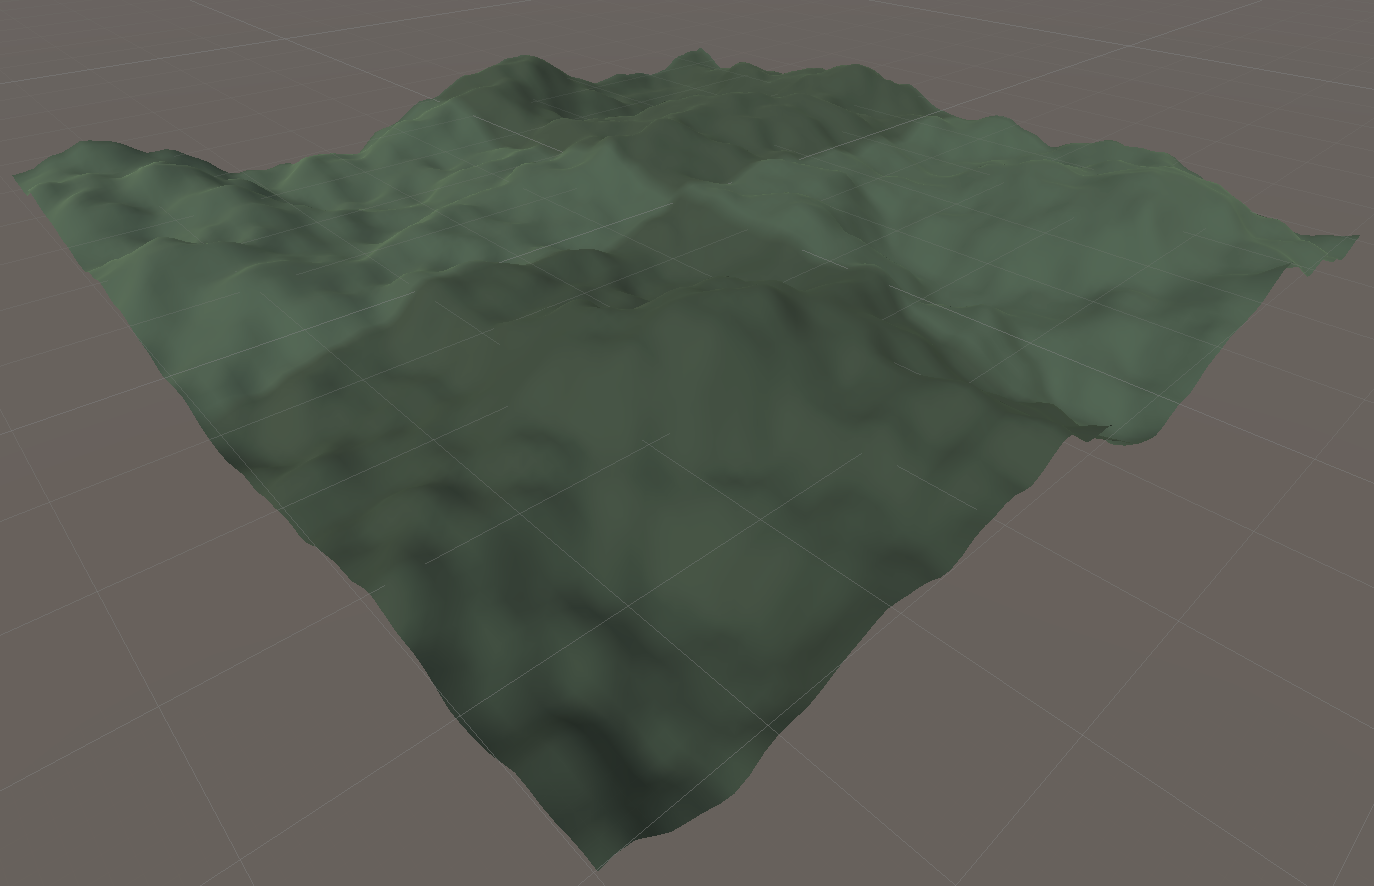
\includegraphics[width=\linewidth]{lacunarity2.png}
        \caption{$l=2$}
        \label{fig:lacunarity2}
    \end{subfigure}
    \hfill
    \begin{subfigure}{0.3\textwidth}
        \centering
        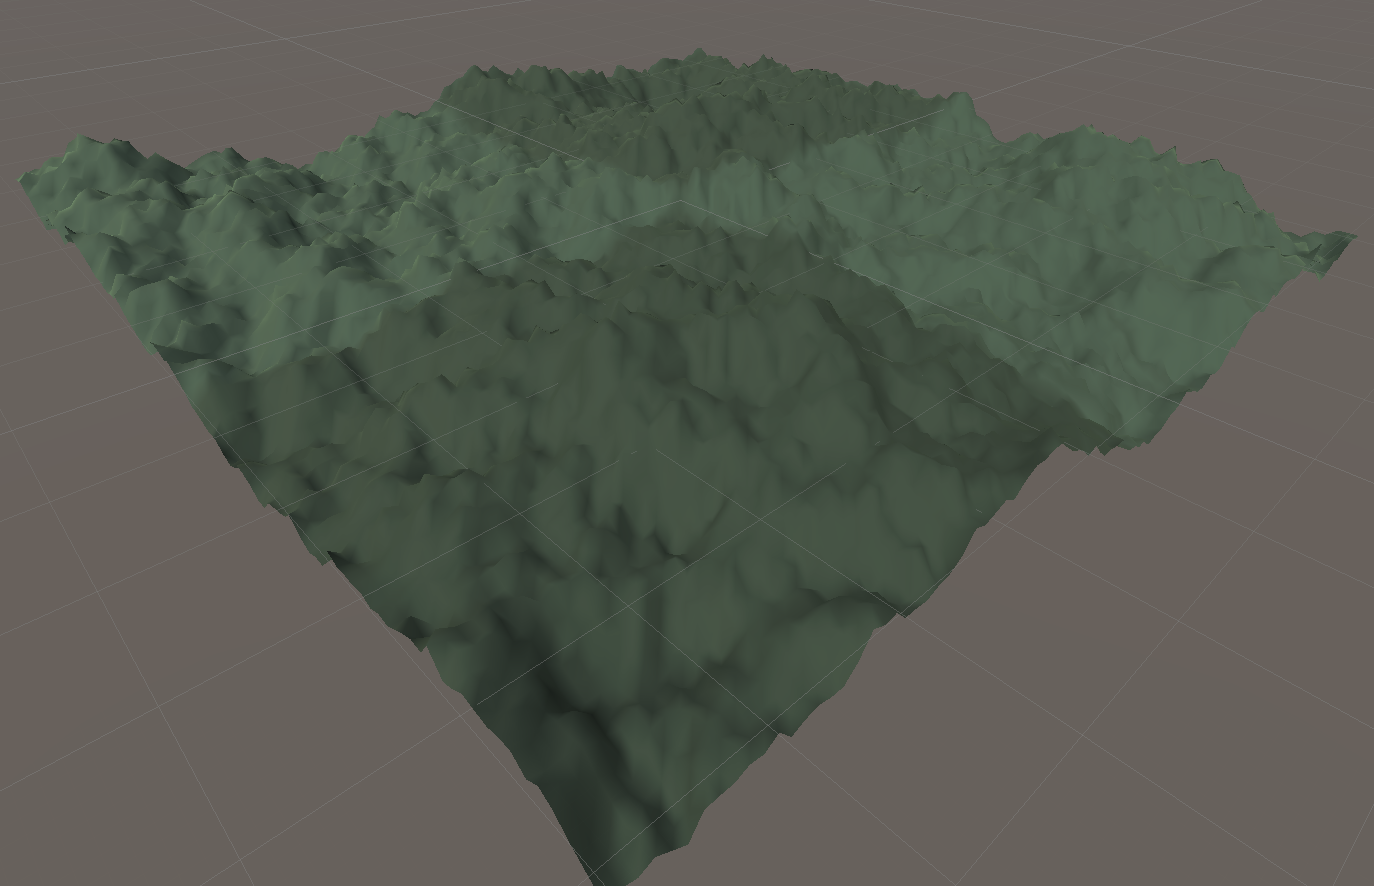
\includegraphics[width=\linewidth]{lacunarity4.png}
        \caption{$l=4$}
        \label{fig:lacunarity4}
    \end{subfigure}
    \caption{The effect of lacunarity on the generated terrain}
    \label{fig:lacunarity}
\end{figure}

Thus, lacunarity, denoted as \(l\), governs the frequency increment across octaves. Specifically, a higher lacunarity value escalates the frequency from one octave to the next, embodying the formula:

$$
\forall x \in \{O_1, O_2, ..., O_n\}, f_x = l^{O_x}
$$

In essence, lacunarity fine-tunes the progression of detail from one octave to another. As illustrated in Figure \ref{fig:lacunarity}, the influence of lacunarity on the terrain is evident over four octaves. An increase in lacunarity amplifies the terrain's detail, rendering it more rugged and intricately textured.

\begin{figure}[ht]
    \centering
    \begin{subfigure}{0.3\textwidth}
        \centering
        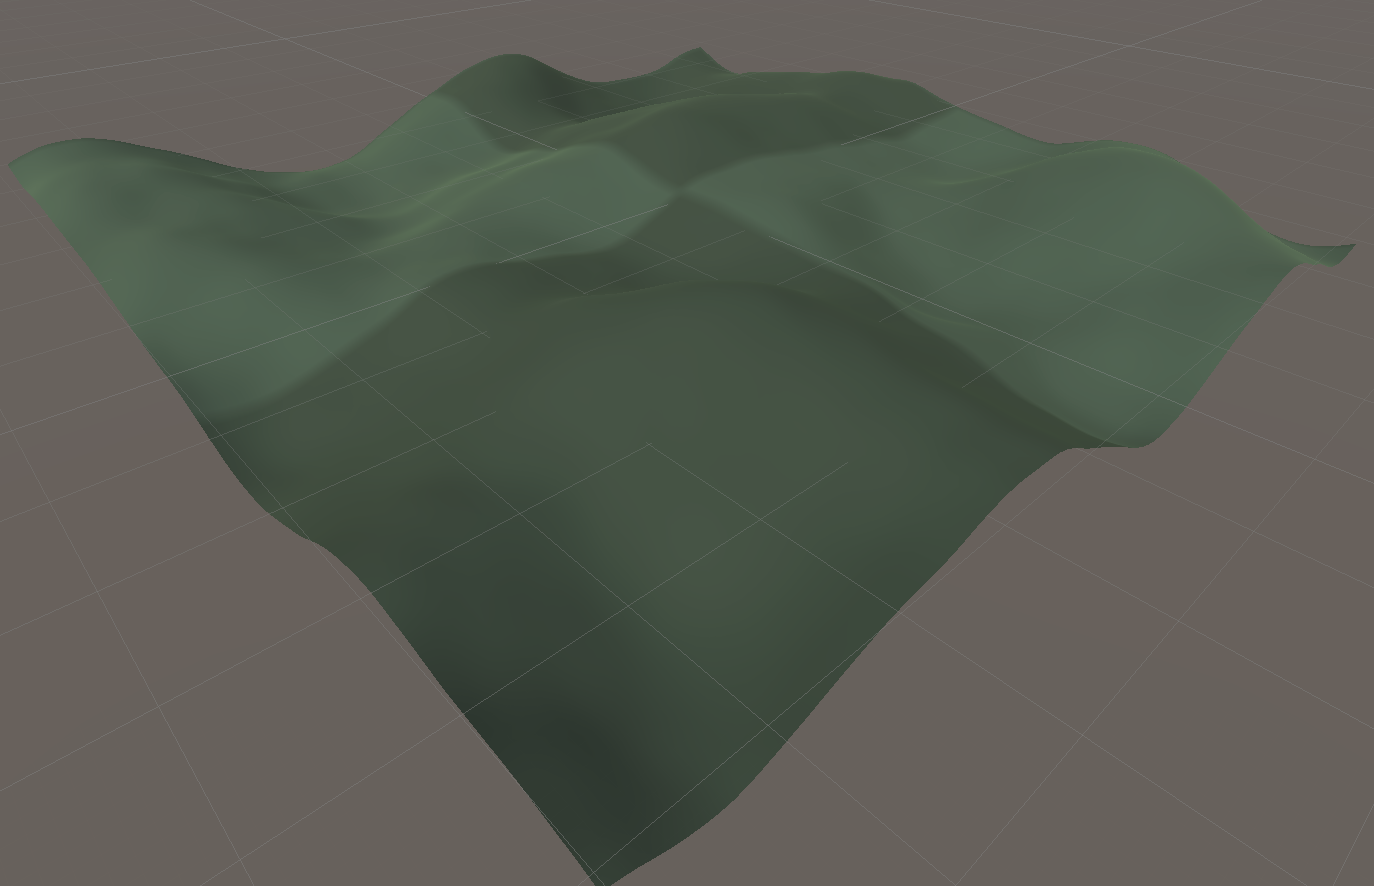
\includegraphics[width=\linewidth]{persistance0.2.png}
        \caption{$p=0.2$}
        \label{fig:persistence0.2}
    \end{subfigure}
    \hfill
    \begin{subfigure}{0.3\textwidth}
        \centering
        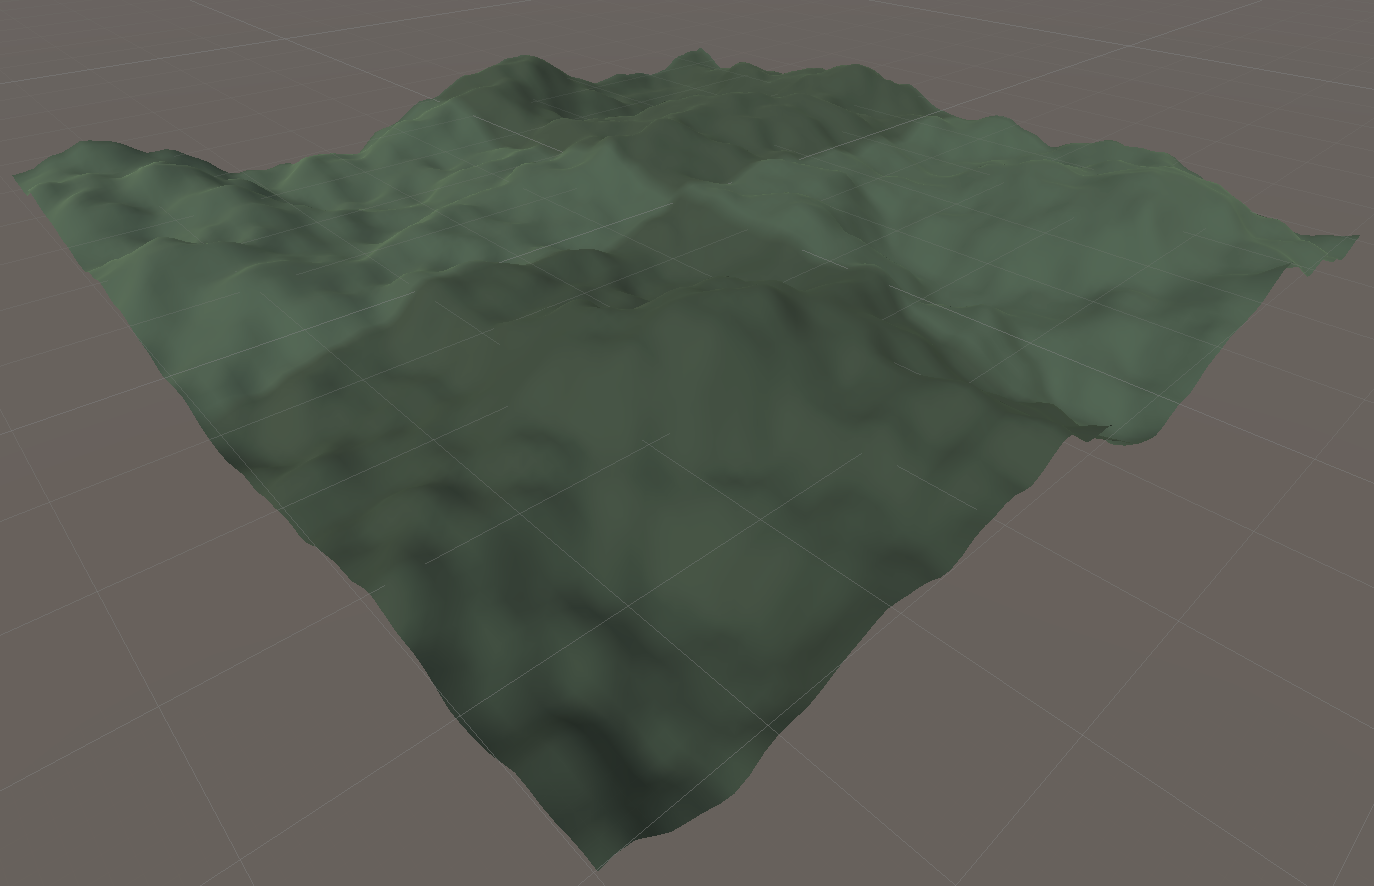
\includegraphics[width=\linewidth]{persistance0.5.png}
        \caption{$p=0.5$}
        \label{fig:persistence0.5}
    \end{subfigure}
    \hfill
    \begin{subfigure}{0.3\textwidth}
        \centering
        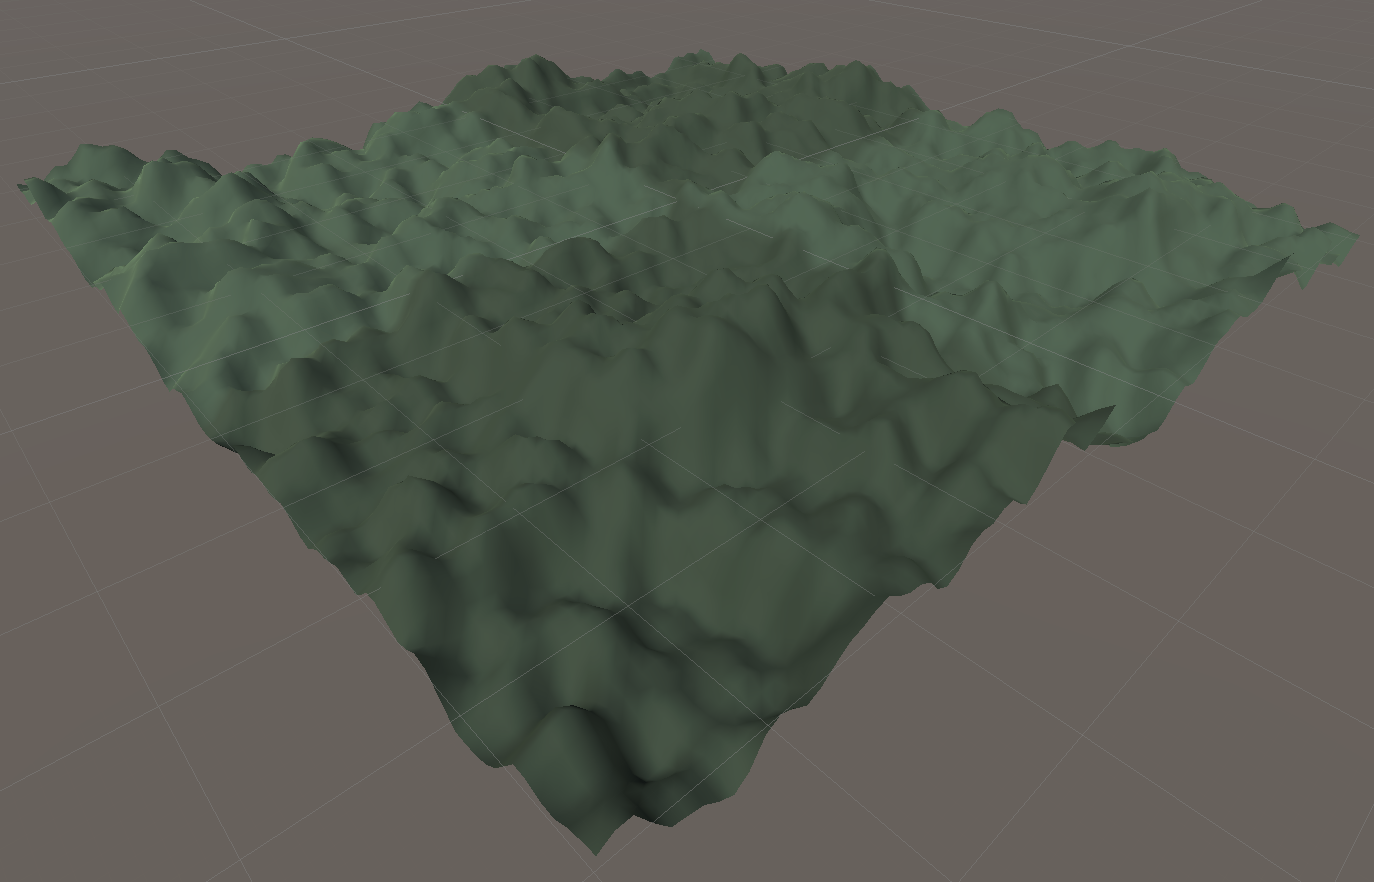
\includegraphics[width=\linewidth]{persistance0.8.png}
        \caption{$p=0.8$}
        \label{fig:persistence0.8}
    \end{subfigure}
    \caption{The effect of persistence on the generated terrain}
    \label{fig:persistence}
\end{figure}

Lastly, the scale parameter, \(s\), dictates the granularity of detail within the waveform when applied to the terrain model. The impact of scale on terrain formation is depicted in Figure \ref{fig:scale}, where an increase in scale leads to a `zoomed out' appearance, rendering the details less notable.

An observable change occurs in the mountain ridge situated in the quadrant nearest to the camera, which becomes larger and more distant from the origin\footnote{Here, the origin refers to the top-left quadrant, positioned furthest from the camera, on the terrain mesh.} as we transition from Figure \ref{fig:scale25} to Figure \ref{fig:scale28}. This effect highlights the scale's role in adjusting the detail level of the terrain's features.

\begin{figure}[ht]
    \centering
    \begin{subfigure}{0.45\textwidth}
        \centering
        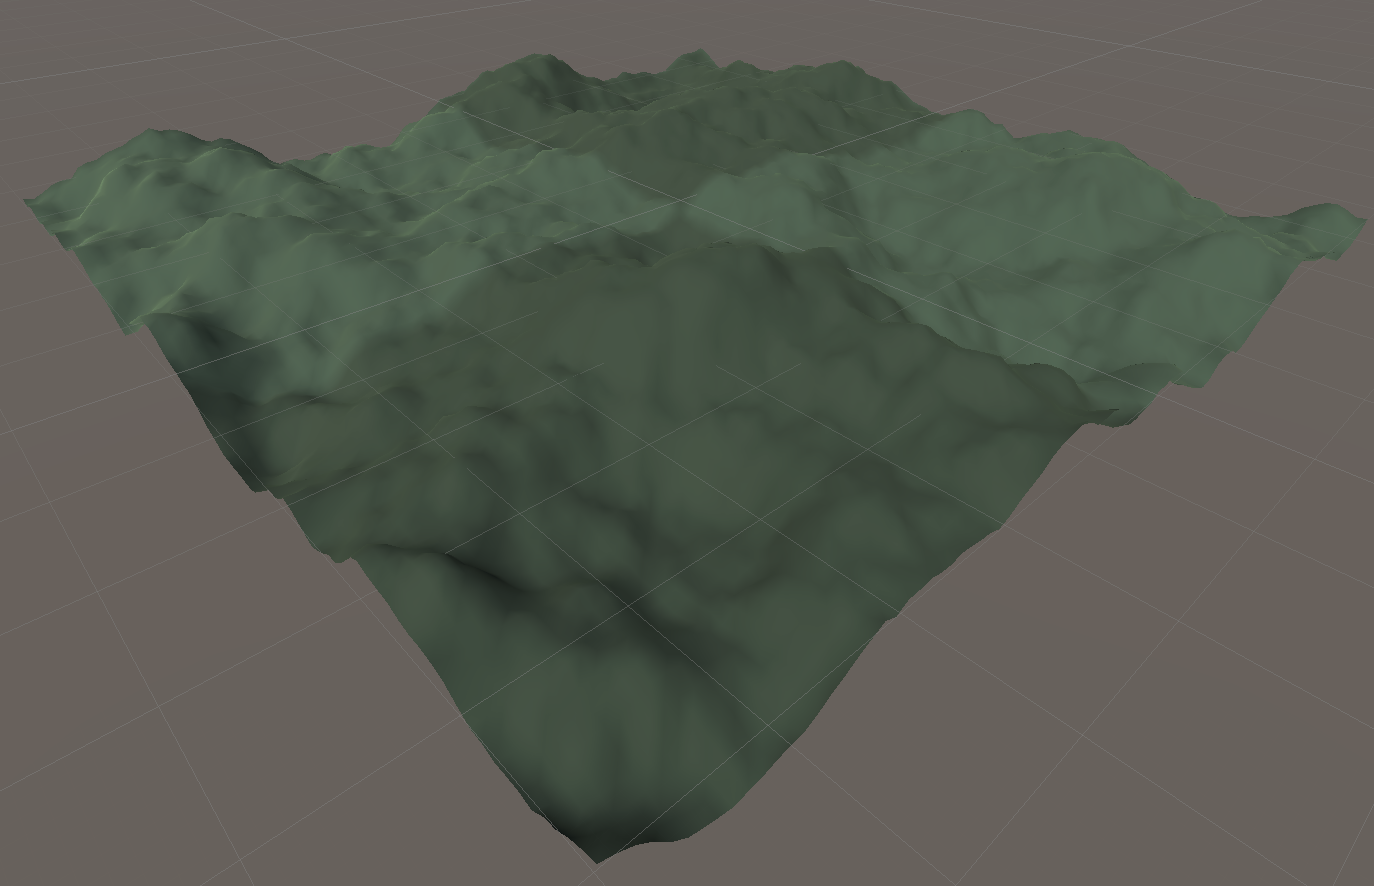
\includegraphics[width=\linewidth]{scale25.png}
        \caption{$s=25$}
        \label{fig:scale25}
    \end{subfigure}
    \hfill
    \begin{subfigure}{0.45\textwidth}
        \centering
        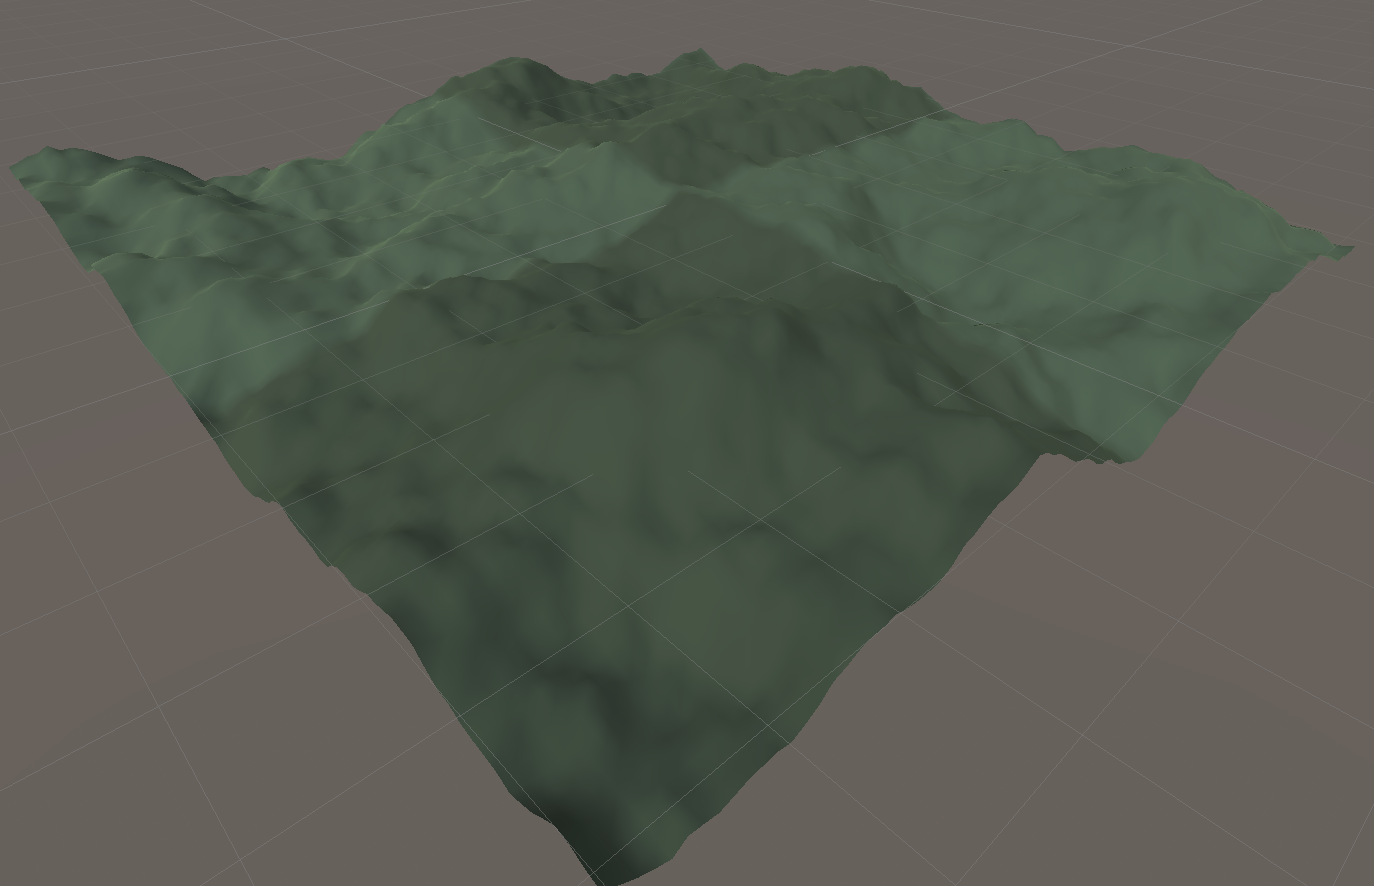
\includegraphics[width=\linewidth]{scale28.png}
        \caption{$s=28$}
        \label{fig:scale28}
    \end{subfigure}
    \caption{The effect of scale on the generated terrain}
    \label{fig:scale}
\end{figure}

When generating the terrain, we can use a seed value to ensure that the terrain generation is repeatable. This means that the same seed value will always produce the same terrain. This feature is useful for debugging, testing, and ensuring consistency across multiple runs of the simulation.

After refining our parameters through empirical testing and insights from \cite[pg.3-4]{Etherington}, we've finalised our terrain mesh, shown in Figure \ref{fig:final}. The terrain mesh is a crucial addition to the simulation, as it allows us to test the agents' ability to avoid obstacles. We will discuss the implementation of terrain avoidance in the next section.

\begin{figure}
    \centering
    \begin{subfigure}{0.4\textwidth}
        \centering
        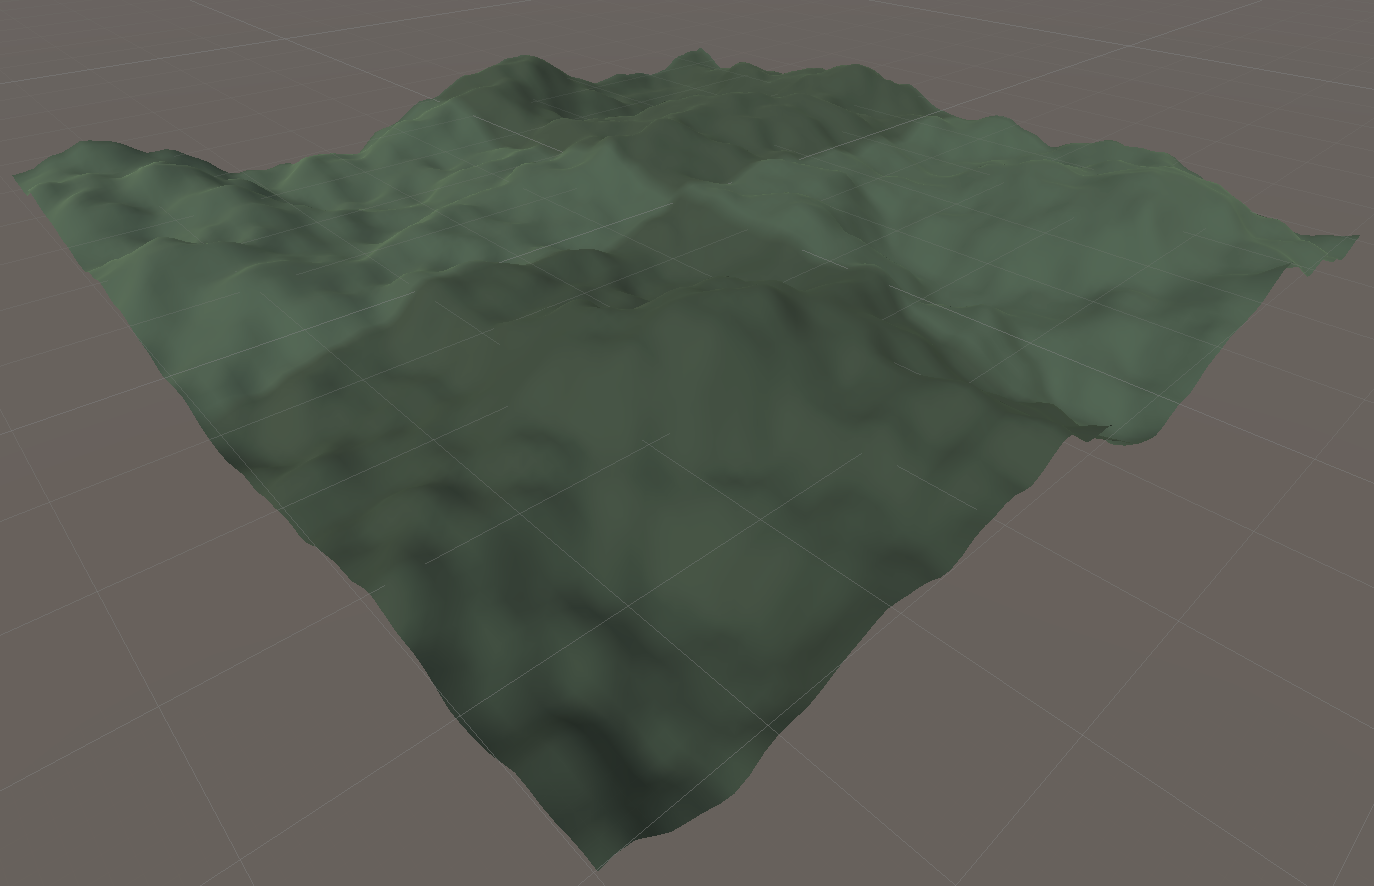
\includegraphics[width=\linewidth]{lacunarity2.png}
        \caption{Final Terrain Mesh}
        \label{fig:final}
    \end{subfigure}
    \hfill
    \begin{subfigure}{0.4\textwidth}
        \centering
        \begin{tabular}{|c|c|}
            \hline
            Parameter & Value \\
            \hline
            Number of Octaves & 4 \\
            \hline
            Lacunarity & 2 \\
            \hline
            Persistence & 0.5 \\
            \hline
            Scale & 25 \\
            \hline
        \end{tabular}
        \caption{Perlin Noise Parameter Values}
        \label{tab:parameter-values}
    \end{subfigure}
    \caption{}
    \label{fig:parameter-values-lacunarity2}
\end{figure}


\subsubsection{Terrain Avoidance}
\label{sec:terrain-avoidance}
Our final additional behaviour, then, will be to implement terrain avoidance. This will allow the agents to avoid the terrain mesh and will be a crucial addition to the agents' autonomy. We will discuss the implementation of this below.

At present, we do not have a method to detect terrain. Common implementations of terrain avoidance in UAVs include the use of LIDAR, radar, or cameras to detect the terrain in front of the UAV\cite{Petrillo,burwell_2019}. 

Given the complexities and computational demands of simulating a LIDAR sensor within our framework, we opt for a more straightforward yet effective solution: a singular ranging sensor. This sensor will project a ray downward from the agent, measuring the distance to the terrain at each simulation frame.

However, this method does impose limitations, particularly a reduced field of view. Unlike many practical applications that offer a 360-degree view, our singular sensor restricts detection to directly beneath the agent. To circumvent terrain obstacles, we propose a method that triggers an upward thrust, $u$ to cause an increase in the agent's local $y$ position, $a_y$, if the distance between the agent and the terrain is less than a given threshold, $t$. We can define this behaviour as follows:

\begin{equation}
    \vec{E} = \begin{bmatrix}
        0 \\
        U \\
        0
    \end{bmatrix}, U =
    \begin{cases}
        \vec{0} & \text{if } a_y > t \\
        u & \text{if } a_y \leq t
    \end{cases}
\end{equation}

For initial testing, we set the threshold, $t$, to 5m and the upward thrust, $u$, to 10. We will adjust these values through empirical testing to ensure the agents can avoid the terrain effectively.

This behaviour is illustrated in Figure \ref{fig:naive-ta-1}, where we observe an agent nearing a steep hill. Initially, up to point 1, the agent maintains its altitude without any adjustments. However, as it approaches point 1 and casts a ray downward, it detects the terrain is closer than the set threshold, resulting in an increase in altitude to avoid the hill. Point 2 marks the hill's crest. Here, the agent realises the gap between itself and the terrain still falls short of safety margins, leading to a further increase in altitude to navigate the obstacle safely.

Further development of this scenario is shown in Figure \ref{fig:naive-ta-2}. Despite recognising the impending terrain, the agent's substantial forward momentum and its resulting tilt impede an effective manoeuvre, leading to a situation where it struggles to clear the hill.

\begin{figure}[ht]
    \centering
    \begin{subfigure}{0.45\textwidth}
        \centering
        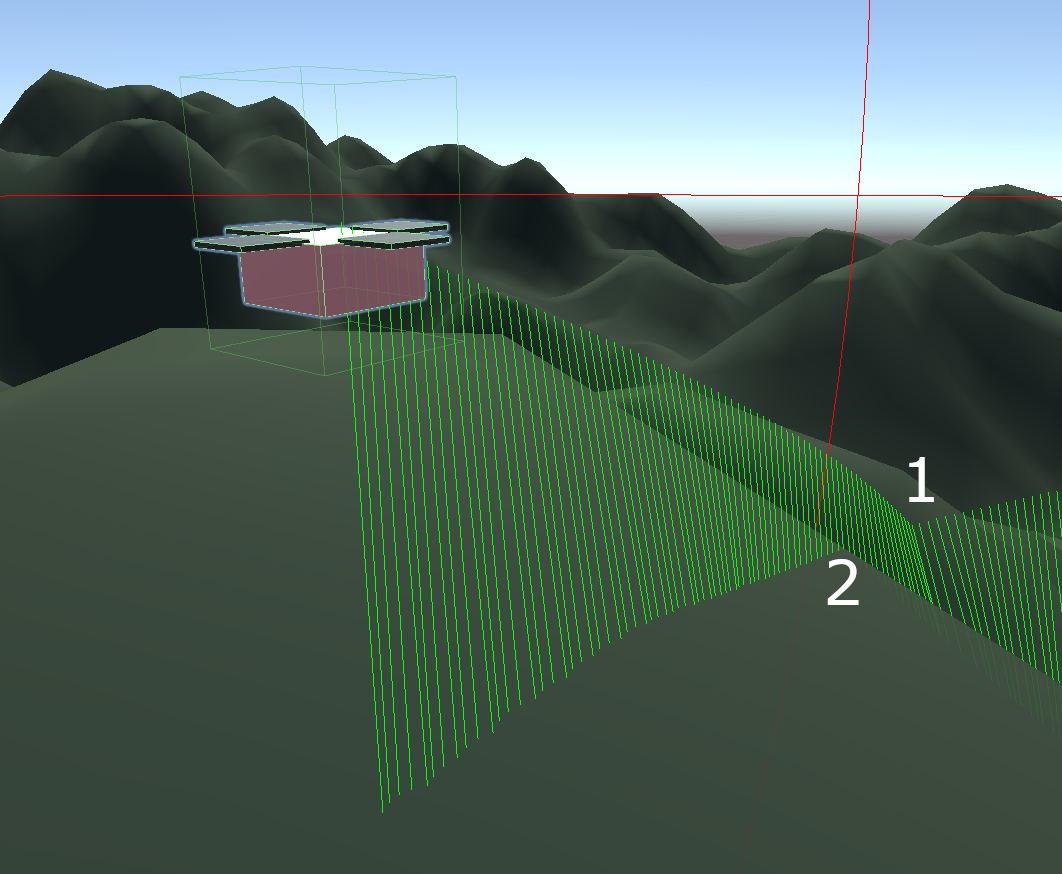
\includegraphics[width=\linewidth]{naive-ta-edited.png}
        \caption{Agent approaching a steep hill}
        \label{fig:naive-ta-1}
    \end{subfigure}
    \hfill
    \begin{subfigure}{0.45\textwidth}
        \centering
        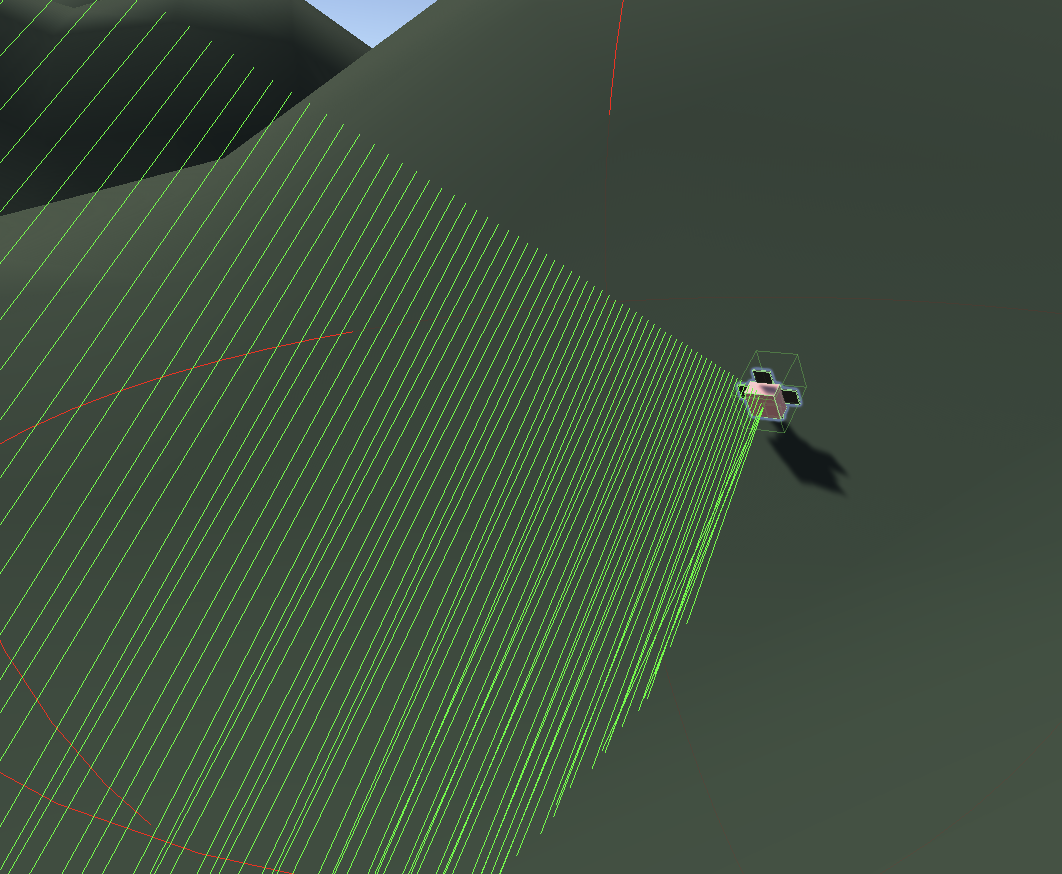
\includegraphics[width=\linewidth]{naive-ta-2.png}
        \caption{Agent failing to avoid terrain}
        \label{fig:naive-ta-2}
    \end{subfigure}
    \caption{Naive Terrain Avoidance}
    \label{fig:naive-ta-side-by-side}
\end{figure}

Our observations highlight deficiencies in the current approach to terrain avoidance, necessitating a refined strategy. To improve the agents' capability for navigating terrain, we propose adjusting the alignment of the ranging sensor to tilt slightly in the direction of the agent's velocity. This adjustment will enable the agent to detect terrain not only directly below but also ahead, significantly enhancing its ability to anticipate and circumvent obstacles.

However, the extensive scale of the terrain presented substantial challenges in optimising avoidance behaviours. A notable limitation in the current framework is the agents' difficulty with steep and large hills, primarily because their avoidance strategy is limited to increasing altitude. This approach is far from ideal; agents should ideally navigate around obstacles rather than merely over them. We intend to explore alternative strategies in Section \ref{sec:lpfe} to overcome this issue.

Alongside these changes in terrain interaction, modifications to how the simulation commences and concludes are also planned. We will introduce two platforms: a red start platform and a green end platform. The start platform is a flat area with a 4-metre radius, situated at the origin, while the end platform, also with a 4-metre radius, will be located at a random point within a 100-metre radius of the origin. 

Agents will start their journey on the start platform and aim to reach the end platform, as illustrated in Figure \ref{fig:platforms}. These adjustments are designed to provide a clear start and end point for the agents, enhancing the structure and coherence of the simulation. 

With behaviours established for agents to navigate complex terrain, our next step is to optimise these behaviours for greater autonomy. This marks a crucial phase, focusing on improving agent independence and efficiency in navigating with minimal oversight, advancing our project towards a more sophisticated and autonomous simulation environment.

\begin{figure}[ht]
\centering
\begin{subfigure}{0.45\textwidth}
    \centering
    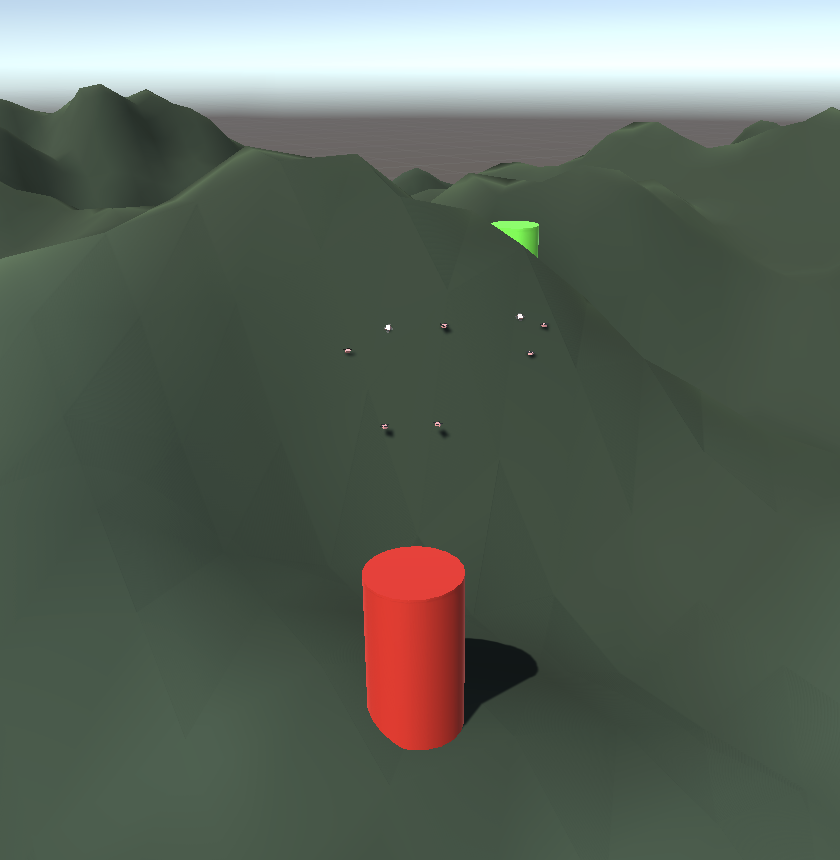
\includegraphics[width=\linewidth]{startplatform.png}
    \caption{Start Platform}
    \label{fig:startplatform}
\end{subfigure}
\hfill
\begin{subfigure}{0.45\textwidth}
    \centering
    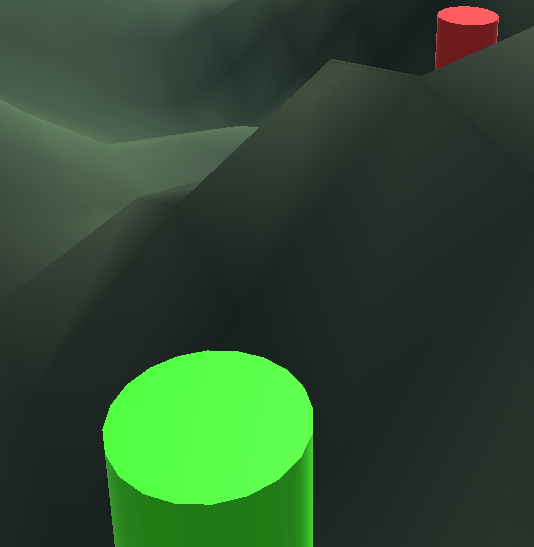
\includegraphics[width=\linewidth]{goalplatform.png}
    \caption{Goal Platform}
    \label{fig:goalplatform}
\end{subfigure}
\caption{Start and Goal Platforms in a single simulation}
\label{fig:platforms}
\end{figure}

\newpage
\section{Methodology}
\label{sec:methodology}

Building on the foundational discussions in Section \ref{sec:introduction} regarding the expansive applications of UAV swarms, we move towards a targeted exploration of optimising the behaviour of the agents. Acknowledging the diverse operational demands on UAVs, we introduce three specific scenarios designed to mirror real-world challenges. These scenarios aim to evaluate the swarms' agility, efficiency, and adaptability under various conditions.

To ensure a comprehensive assessment, we've established a set of metrics. These will critically inform the development of an advanced cost function targeted for optimisation. This step marks a significant stride towards refining UAV behaviours, ensuring their effectiveness across a range of applications and edging us closer to realising the extensive capabilities of autonomous UAV swarms.

\subsection{Scenario 1: Shortest First Arrival Time}
Firstly, we will consider the scenario where reaching the goal in the shortest time is the most important factor. This is a present requirement for time-sensitive situations, where the redundancy of multiple agents is used to ensure that the goal is reached as quickly as possible. In essence, it means agents can take more risks in their behaviour to achieve the objective.

Some example situations where this scenario would be of use include military operations in hostile environments, gaining situational awareness in disaster zones, and surveying hazardous environments\cite{Srinath}. For the simulations of this scenario, we will consider the following metrics:

\paragraph{First Arrival Time} 
We must consider the time taken for the first agent to reach the goal; it is the primary objective of the agents in this scenario. Specifically, this is the time taken for the first agent to enter the goal radius as defined in Section \ref{sec:goal-seek}. We define a simulation run time, which will be the length a simulation is allowed to run for.

For the purposes of normalisation, we will use the time taken for the first agent to reach the goal, divided by the simulation run time. This will give us a value between 0 and 1, where a lower number indicates a better performance.This is the primary objective of the agents in this scenario, so we will give it a larger weight in our cost function.

\paragraph{Proportion of Agents Arriving} A simulation run where more agents arrive at the goal is more successful than one where fewer agents arrive. Furthermore, a simulation run where no agents arrive would be considered a failure.

We will then, also consider the proportion of agents that do not arrive at the goal by the simulation run time. This will give us a value between 0 and 1, where a lower number indicates a better performance. This is a secondary objective of the agents in this scenario.

\subsection{Scenario 2: Reduced Spread (Cohesivity)}
This scenario aims to reduce the spread of the agents in the flock. This is important in situations where the agents must maintain a close formation, such as in search and rescue operations, or in the delivery of goods. A simulation run's success in this scenario will be dependent on two metrics:

\paragraph{Standard Deviation of Arrival Times} We will consider the times at which the agents arrive at the goal, for all agents that arrive before the simulation run time. We will then calculate the standard deviation of these times. A lower standard deviation indicates that the agents are arriving at the goal more uniformly. We will give this metric a larger weighting in our cost function.

A key issue with this metric is that it does not consider the method by which the agents arrive at the goal. For example, if all agents arrive at the goal at the same time, the standard deviation will be 0. This does not necessarily imply that the agents are in a close formation.

\paragraph{First Arrival Time} As with the first scenario, we still consider the time taken for the first agent to reach the goal. A run where all agents reach the goal with a low standard deviation between them, but take a long time to do so is suboptimal. We will give this metric a smaller weighting in our cost function.

\paragraph{Proportion of Agents Arriving} As with the first scenario, we will consider the proportion of agents that do not arrive at the goal by the simulation run time. We do this to ensure that the cost function accounts for the number of agents within an arriving group.

\subsection{Scenario 3: Reducing Collision Numbers}
This scenario aims to reduce the number of collisions between agents and between agents and other objects in the environment. This is important in situations where the agents must operate in close proximity to each other, such as in the delivery of goods, or the area monitoring. We will consider both the arrival time of the first agent and the proportion of agents that arrive at the goal, as in the previous scenarios, to a small extent, for similar reasons as justified previously.

We will also consider the following metrics: 

\paragraph{Number of Collisions} We will consider the number of collisions that occur between agents and between agents and objects in the environment. A simulation run where fewer collisions occur is more successful than one where more collisions occur. We will give this metric a larger weighting in our cost function.

\newpage
\section{Optimisation}
Earlier, we utilised an empirical method to optimise our initial three behaviours. However, we note that for each extra parameter we introduce, the complexity of the parameter space increases exponentially. Consider an example in which each parameter is bounded by integers within the inclusive range $(0,10)$. With 3 parameters, this is a three-dimensional parameter space with $11^3 = 1331$ possible combinations. With 5 parameters, this is a five-dimensional parameter space with $11^5 = 161051$ possible combinations. This is a combinatorial explosion, and it is not feasible to optimise the parameters in this way.

In the quest for more scalable optimisation techniques, we explore two prominent probabilistic methods. The first is genetic algorithms, inspired by natural selection, which have shown promise in the field of swarm robotics behaviour optimisation. A significant study by \citet{Alaliyat2014OptimisationOB} demonstrated the application of a genetic algorithm to optimise a Boids model, though it is notably computation-intensive.

An alternative approach is the hill climbing algorithm—more accurately termed gradient descent in our context, aimed at minimising the cost function. This method iteratively refines a solution by adjusting a single parameter incrementally. While less computationally demanding than genetic algorithms, hill climbing risks getting trapped in local minima, potentially missing the global minimum.

Given these considerations, our focus shifts to exploring an alternative optimisation strategy that can efficiently navigate the expansive parameter space to identify optimal settings.

\subsection{Simulated Annealing}
\label{sec:simulated-annealing}
The method we will use to optimise the parameters is simulated annealing. This is a probabilistic method that is used to find the global minimum of a function within a given search space. It is based on the physical process of annealing, where a material is heated and then cooled slowly to remove defects and reduce the material's energy. It is, in principle, a more advanced version of the hill climbing algorithm which can overcome local minima.

The simulated annealing algorithm begins its search from a randomly selected point within the search space, proceeding to explore the neighbouring points. For each neighbour, the algorithm evaluates the cost function, denoted as \(t\). Movement to this new point from the current position is determined by comparing their cost functions. When the new point offers a lower cost, indicating an improvement, the algorithm naturally transitions to it. Conversely, if the new point's cost is higher, suggesting a step back, the algorithm may still move to this point with a probability influenced by the cost function increase, \(|c(t) - c(t+1)|\), and a temperature parameter, \(T\). This probabilistic acceptance is key for the algorithm's ability to navigate out of local minima by occasionally accepting worse solutions temporarily.

The method of temperature reduction, or the cooling schedule, plays a pivotal role in the success of the algorithm. The temperature parameter \(T\)  dictates the algorithm's readiness to accept suboptimal moves; as \(T\) decreases, the algorithm becomes increasingly picky, reducing the probability of accepting higher-cost solutions. 

The cooling schedule must strike a careful balance: a rapid reduction in temperature can lead the algorithm to settle prematurely on local minima, while too slow a decrease can result in an inefficient search that takes too long to converge to an optimal solution. Adopting a linear cooling schedule allows the temperature to decrease steadily with each iteration, aiming to guide the algorithm towards global optimality with an effective balance between exploration and exploitation.

We will define our acceptance function, $P \in (0,1)$ as follows:

\begin{equation}
    P = \begin{cases}
        1 & \text{if } c(t+1) < c(t) \\
        e^{-\frac{c(t+1) - c(t)}{T}} & \text{if } c(t+1) \geq c(t)
    \end{cases}
\end{equation}

The exponential term in the simulated annealing algorithm's acceptance function draws inspiration from the Boltzmann distribution - a concept from statistical mechanics. This distribution helps predict how likely a system is to be found in a certain state, based on its energy level. The formula for the Boltzmann distribution is:

\begin{equation}
    P(i) = e^{-\frac{E_i}{kT}}
\end{equation}

Here, \(P(i)\) represents the likelihood of the system occupying a state with energy \(E_i\), given a temperature \(T\) and the Boltzmann constant \(k\). This equation essentially tells us that at higher temperatures, a system is more likely to be found in states of higher energy due to particles moving more vigorously and exploring a broader range of states.

Translating this concept into the realm of simulated annealing and optimisation, we can think of the `energy' of a system as analogous to the cost of a solution; the lower the energy, the better the solution. The `temperature' in our algorithm simulates the physical temperature, controlling how willing the algorithm is to explore solutions of varying quality. At high temperatures, similar to particles in a heated system, the algorithm is more open to exploring less optimal solutions, increasing the chance of escaping local minima. As the temperature cools, the algorithm becomes more discerning, progressively favouring solutions that lower the "energy" or improve the optimization, guiding it towards the global minimum.

This clever use of mechanics principles in a computational algorithm allows for a more dynamic and effective search for optimal solutions, embodying the idea that sometimes, taking a step back (or exploring higher-cost solutions) can ultimately lead to finding the best path forward.

We can then define our parameters and our cost function. As noted previously in Section \ref{sec:combining-behaviours}, the parameter space can be defined as a linear combination of the behaviours and their weights. For clarity, we now redefine this in terms of our extended parameter space, which includes goal-seeking and terrain avoidance behaviours.

\begin{equation}
\vec{V} = 
\alpha
\begin{bmatrix}
    x_{avoid} \\
    y_{avoid} \\
    z_{avoid} \\
\end{bmatrix}
+ \beta
\begin{bmatrix}
    x_{align} \\
    y_{align} \\
    z_{align} \\
\end{bmatrix}
+ \gamma
\begin{bmatrix}
    x_{cohere} \\
    y_{cohere} \\
    z_{cohere} \\
\end{bmatrix}
+ \delta
\begin{bmatrix}
    x_{seek} \\
    y_{seek} \\
    z_{seek} \\
\end{bmatrix}
+ \epsilon
\begin{bmatrix}
    x_{terrain} \\
    y_{terrain} \\
    z_{terrain} \\
\end{bmatrix}
\end{equation}

We can then define our cost function, which is a linear combination of the metrics defined in Section \ref{sec:methodology}. We will define a singular, modular cost function to allow for the easy addition of new metrics and the ability to tweak the weighting of the existing metrics. 

The cost function will normalise the given weights, and the given metrics will also be normalised to ensure the output of the cost function lies in the range $(0,1)$. Specifically, we define the normalisation of the four weights as:
\begin{equation}
    \forall w_i \in W, w_i = \frac{w_i}{\sum_{i=1}^{|W|}{w_i}}
\end{equation}

We also define the normalised metrics as follows:

\paragraph{First Arrival Time}
We can normalise this value by dividing it by the simulation time (the length the simulation is allowed to run for). Hence,

\begin{equation}
    m_1 = \frac{\text{firstArrivalTime}}{\text{simulationRuntime}}
\end{equation}

\paragraph{Proportion Reached}
In a similar nature to the normalisation method for the \emph{first arrival time} metric, we can divide the number of agents that have not reached the goal by the simulation time by the total number of agents in the simulation, namely:

\begin{equation}
    m_2 = \frac{\text{numberOfAgents} - \text{numberOfAgentsReached}}{\text{numberOfAgents}}
\end{equation}

\paragraph{Number of Collisions}
Normalising a metric that has, in theory, no upper bound, is a challenge. In this case, we will look at fitting the data to a bounded function. The \emph{logistic function} is a good candidate for this. The logistic function is defined as:

\begin{equation}
    f(x) = \frac{1}{1 + e^{-k(x-x_0)}}
\end{equation}

Specifically, we can set the midpoint value of the function, $x_0$, to be the mean of the number of collisions over an example set of simulations, such that $f(x_0) = 0.5$. We determined this to be $\approx 40$ collisions. We can then set the steepness of the function, $k$, to be 0.1. This will give us a function that is bounded between 0 and 1 and is steep enough to give a good approximation of the number of collisions.


\paragraph{Standard Deviation of Arrival Times}

An upper bound on the standard deviation, $\sigma$, of a population is the population range. We can then normalise the standard deviation of the arrival times by dividing it by the range of the possible arrival times, which is equal to the simulation runtime.

A caveat here is that if no agents arrive at the goal, the standard deviation will be 0, which would set the normalised value to 0. This is not ideal, as the agents have not arrived at the goal. We will consider this as an edge case and set the normalised value to 1 in this case. Hence, we can define the normalised standard deviation of arrival times as:

\begin{equation}
    m_4 = \begin{cases}
        1 & \text{if } \sigma = 0 \\
        \frac{\sigma}{\text{simulationRuntime}} & \text{otherwise}
    \end{cases}
\end{equation}

We can then represent our cost function as a function that returns a weighted sum of the normalised metrics:

\begin{equation}
    C(W,M) = w_1m_1 + w_2m_2 + w_3m_3 + w_4m_4
\end{equation}

At this stage, it is important to note the disjoint nature of the parameters (inputs) and metrics (observations). The simulation is non-deterministic, due to small fluctuations in starting positions and randomised goal positions. To help mitigate this, we will introduce our simulation process in the next section.

\subsection{Simulations}
To refine our parameter settings effectively, we embark on a series of simulations for each parameter set, aiming to capture the average performance metrics across multiple runs. This approach helps mitigate the inherent randomness in simulation outcomes, providing a more robust basis for evaluating and refining our UAV swarm optimisation strategies.

Achieving the right balance in the number of simulations per parameter set is crucial. Too few simulations may lead to significant variance in the metrics, compromising the accuracy of our cost function. Conversely, conducting too many simulations can incur excessive computational overhead. To strike this balance, we initially opted for 10 simulations per parameter set, with the flexibility to adjust this number based on the insights gained from our initial simulation results.

Our parameter space, bounded between 0 and 20 for each parameter, is systematically explored with a step size of 0.5. This granularity allows us to thoroughly sample the parameter space, ensuring comprehensive coverage without overwhelming computational resources. In defining the neighbourhood of a parameter set, we consider adjustments of $\pm 0.5$ for each parameter, facilitating an efficient exploration of nearby solutions.

As for the cooling schedule employed in simulated annealing, we tailor it to the remaining simulations to be executed. For instance, in a scenario involving 500 iterations comprising 10 simulations each, the initial temperature is set to 500, decreasing by 1 after each simulation. This linear reduction ensures a gradual cooling process, effectively guiding the algorithm towards optimal solutions while efficiently utilising computational resources.

\subsection{Results}
A varying number of simulations were run for each scenario. In this section, we explore the results and discuss the potential reasons for the outcomes.

\subsubsection{Scenario 1: Shortest First Arrival Time}
Within this scenario, we meticulously conducted 821 valid iterations, complemented by several strategic restarts to ensure the robustness of our findings. Such restarts are paramount in simulations to prevent potential biases or anomalies within the data set, thus enhancing the reliability of the results. The core objective of this scenario is to optimise the swarm's efficiency in achieving the designated target in the shortest possible time. This goal is crucial for the practical deployment of UAV swarms in scenarios such as emergency response or rapid reconnaissance, where time is of the essence.

The analysis hinges on the detailed observation of the cost function's behaviour throughout the iterations. As illustrated in Fig. \ref{fig:scenario1-cost}, a notable observation is the appearance of a global minimum around iteration 300. A closer inspection within this range reveals a gradual reduction in the cost function over time, indicative of the algorithm's effective optimization process. 

Interestingly, around iteration $\approx 250$, there is a discernible increase in the cost function. This phenomenon is attributed to the algorithm's strategic exploration of the parameter space, allowing it to escape a potential local minimum. Such exploration is instrumental in the discovery of a more optimal solution, underscoring the algorithm's adaptive capability in navigating the complex parameter landscape.

Analysing the weight assignments indicated in Table \ref{tab:scenario1-parameters} reveals that the seeking behaviour is accorded the highest weight. This prioritisation aligns with the scenario's primary objective, where the swift attainment of the goal location is prioritised. 

Additionally, the terrain avoidance behaviour is also assigned a high weight, reflecting the necessity to navigate complex terrain meshes efficiently. In contrast, the alignment and cohesion behaviours are assigned lower weights. This weighting strategy underscores the relatively lesser importance of these behaviours in the context of this specific scenario, where the primary focus is on expedient target location rather than the maintenance of formation or collective movement. 

\begin{figure}[ht] 
    \centering
    \begin{subfigure}{.4\textwidth}
    \begin{tikzpicture}[trim axis left, trim axis right]
        \begin{axis}[
            xlabel=Iteration,
            ylabel=Cost,
            no markers
        ]
        
        \addplot table [x expr=\coordindex, y=tcost, col sep=comma] {scenario1.csv};
        
        \end{axis}
    \end{tikzpicture}
    \end{subfigure}
    \hfill
    \begin{subfigure}{.4\textwidth}
        \begin{tikzpicture}[trim axis left, trim axis right]
            \begin{axis}[
                xlabel=Iteration,
                ylabel=Cost,
                no markers,
                xmin=200,
                xmax=300
            ]
            
            \addplot table [x expr=\coordindex, y=tcost, col sep=comma] {scenario1.csv};
            
            \end{axis}
        \end{tikzpicture}
    \end{subfigure}
    \caption{Cost Function over Iterations for Scenario 1}
    \label{fig:scenario1-cost}
\end{figure}


\begin{table}[ht]
    \centering
    \begin{tabular}{|c|c|}
        \hline
        Parameter & Weight \\
        \hline
        Avoidance & 8.5 \\
        \hline
        Alignment & 2.5 \\
        \hline
        Cohesion & 0.5 \\
        \hline
        Seeking & 17 \\
        \hline
        Terrain Avoidance & 16.5 \\
        \hline \hline
        Cost & 0.268 \\
        \hline
    \end{tabular}
    \caption{Optimal Parameters for Scenario 1}
    \label{tab:scenario1-parameters}
\end{table}

\subsubsection{Scenario 2: Reduced Spread (Cohesivity)}
A total of 1214 runs were completed for this scenario, again, with several restarts throughout. The cost function over the iterations is shown in Fig. \ref{fig:scenario2-cost}. The zoomed-in section shows the global minimum at the 226th iteration, of which the parameter values are detailed in Table \ref{tab:scenario2-parameters}.

Fig. \ref{fig:scenario2-cost} shows some peculiar behaviour with the cost function, namely, that it appears to consistently fluctuate between two collections of values, centred at $\approx 0.37$ and $\approx 0.31$. We also notice that the general trend of the cost function before approaching the determined global minimum is not strongly negative.

To attempt to mitigate this, the simulation environment was tweaked, increasing the number of simulations per iteration from 10 to 100. The results for this set of simulations are shown in Fig. \ref{fig:scenario2-cost-100}. These results indicate the problem persists, but the outliers present from the previous runs (where the cost function evaluated to a value not centred around the poles at $\approx 0.31, 0.37$) have been reduced.

\begin{figure}[ht]

    \centering
    \begin{subfigure}{.4\textwidth}
    \begin{tikzpicture}[trim axis left, trim axis right]
        \begin{axis}[
            xlabel=Iteration,
            ylabel=Cost,
            no markers,
            xmax=1215
        ]
        
        \addplot table [x expr=\coordindex, y=tcost, col sep=comma] {scenario2.csv};
        
        \end{axis}
    \end{tikzpicture}
    \end{subfigure}
    \hfill
    \begin{subfigure}{.4\textwidth}
        \begin{tikzpicture}[trim axis left, trim axis right]
            \begin{axis}[
                xlabel=Iteration,
                ylabel=Cost,
                no markers,
                xmin=180,
                xmax=230
            ]
            
            \addplot table [x expr=\coordindex, y=tcost, col sep=comma] {scenario2.csv};
            
            \end{axis}
        \end{tikzpicture}
    \end{subfigure}
    \caption{Cost Function over Iterations for Scenario 2}
    \label{fig:scenario2-cost}

\end{figure}

\begin{table}[ht]
    \centering
    \begin{tabular}{|c|c|}
        \hline
        Parameter & Weight \\
        \hline
        Avoidance & 12.5 \\
        \hline
        Alignment & 4 \\
        \hline
        Cohesion & 15 \\
        \hline
        Seeking & 18.5 \\
        \hline
        Terrain Avoidance & 0.5 \\
        \hline \hline
        Cost & 0.229 \\
        \hline
    \end{tabular}
    \caption{Optimal Parameters for Scenario 2}
    \label{tab:scenario2-parameters}
\end{table}

\begin{figure}[ht]
    \centering
    \begin{tikzpicture}[trim axis left, trim axis right]
        \begin{axis}[
            xlabel=Iteration,
            ylabel=Cost,
            no markers,
            width=0.8\textwidth,
            height=0.4\textwidth,
        ]
        
        \addplot table [x expr=\coordindex, y=tcost, col sep=comma] {scenario2b.csv};
        
        \end{axis}
    \end{tikzpicture}
    \caption{Cost Function over Iterations for Scenario 2 with 100 Simulations}
    \label{fig:scenario2-cost-100}
\end{figure}

To delve deeper into what was causing this, the metrics themselves were analysed for a set of iterations. Fig. \ref{fig:scenario2-metrics} shows the metrics over one set of annealing. We would expect the values of both metrics to decrease over time, as the cost function is minimised. However, while we can see the variance of the \emph{first arrival time} metric decrease over time, as expected, due to the temperature decrease in the algorithm, the \emph{standard deviation of arrival times} metric does not show a clear trend. 

This is likely the cause of the fluctuating cost function, and a key reason explaining why this behaviour was not present in the results of the first scenario. We will hypothesise why this occurs in Section \ref{sec:results-discussion}.

\begin{figure}[ht]
    \centering
    \begin{tikzpicture}[trim axis left, trim axis right]
        \begin{axis}[
            xlabel=Iteration,
            ylabel=Metric Value,
            no markers,
            width=0.8\textwidth,
            height=0.4\textwidth,
            ymax=40
        ]

        \addplot table [x expr=\coordindex, y=TimeReached, col sep=comma] {metrics2.csv};
        \addplot table [x expr=\coordindex, y=Sigma, col sep=comma] {metrics2.csv};

        \addlegendentry{Time Reached (s)};
        \addlegendentry{$\sigma$};
        
        \end{axis}
    \end{tikzpicture}
    \caption{Metrics over Iterations for Scenario 2}
    \label{fig:scenario2-metrics}
\end{figure}

\subsubsection{Scenario 3: Reducing Collision Numbers}
A total of 508 runs were completed for this scenario, with several restarts. The cost function over the iterations is shown in Fig. \ref{fig:scenario3-cost}. The zoomed-in section shows the global minimum at the 186th iteration, of which the parameter values are detailed in Table \ref{tab:scenario3-parameters}.

The results for this scenario again show peculiar behaviour. It would be expected for the avoidance behaviour to have a higher weight than the alignment and cohesion behaviours, given the primary objective of the agents in this scenario. However, the alignment and cohesion behaviours have higher weights. We will discuss this in Section \ref{sec:results-discussion}.

\begin{figure}[ht]
    \centering
    \begin{subfigure}{.4\textwidth}
    \begin{tikzpicture}[trim axis left, trim axis right]
        \begin{axis}[
            xlabel=Iteration,
            ylabel=Cost,
            no markers
        ]
        
        \addplot table [x expr=\coordindex, y=tcost, col sep=comma] {scenario3.csv};
        
        \end{axis}
    \end{tikzpicture}
    \end{subfigure}
    \hfill
    \begin{subfigure}{.4\textwidth}
        \begin{tikzpicture}[trim axis left, trim axis right]
            \begin{axis}[
                xlabel=Iteration,
                ylabel=Cost,
                no markers,
                xmin=140,
                xmax=188
            ]
            
            \addplot table [x expr=\coordindex, y=tcost, col sep=comma] {scenario3.csv};
            
            \end{axis}
        \end{tikzpicture}
    \end{subfigure}
    \caption{Cost Function over Iterations for Scenario 3}
    \label{fig:scenario3-cost}
\end{figure}

\begin{table}[ht]
    \centering
    \begin{tabular}{|c|c|}
        \hline
        Parameter & Weight \\
        \hline
        Avoidance & 3 \\
        \hline
        Alignment & 15 \\
        \hline
        Cohesion & 15.5 \\
        \hline
        Seeking & 4.5 \\
        \hline
        Terrain Avoidance & 2.5 \\
        \hline \hline
        Cost & 0.202 \\
        \hline
    \end{tabular}
    \caption{Optimal Parameters for Scenario 3}
    \label{tab:scenario3-parameters}
\end{table}

% potential to talk more here about the metric values

\subsection{Sensitivity Analysis}
We will now consider the sensitivity of the cost function to the weights of the metrics by exploring the nearby parameter space of the optimal parameters found in the previous section. We will do this by varying the weights of the metrics by $\pm 0.5$ and observing the change in the cost function. We will do this solely for the first scenario, as the results for the other scenarios are less intuitive.

Fig. \ref{fig:spiderweb}\footnote{The cohesion metric is not modified in the negative direction, as it is already set at the minimum value of 0.5.} shows the sensitivity of the cost function to the weights of the metrics. Visually, opposite axes in the spider diagram show the polarity of the change. The lengths of the axes represent the difference between the cost function at the optimal parameters and the cost function at the parameters with the weights of the metrics increased or decreased by $\pm 0.5$.

This results in a `topological' view of the sensitivity of the cost function to the weights of the metrics at the point of the determined global minimum. We can see that this scenario seems sensitive to changes in the alignment and avoidance behaviours most. On the contrary, it seems less sensitive to the seeking behaviour. To this end, we have likely found an optimal set of parameters in the more sensitive dimensions. 

It is vital to note that the values of the sensitivity analysis may be dependent on external factors. Namely, the nondeterministic nature of the simulation may cause the sensitivity of the cost function to the weights of the metrics to vary; the results are likely to be different if the simulation was run a different number of times.

\newcommand{\D}{10} % number of dimensions (config option)
\newcommand{\U}{13} % number of scale units (config option)

\newdimen\R % maximal diagram radius (config option)
\R=6cm 
\newdimen\L % radius to put dimension labels (config option)
\L=6.5cm

\newcommand{\A}{360/\D} % calculated angle between dimension axes  

\begin{figure}[ht]
 \centering

\begin{tikzpicture}[scale=1]
  \path (0:0cm) coordinate (O); % define coordinate for origin

  % draw the spiderweb
  \foreach \X in {1,...,\D}{
    \draw (\X*\A:0) -- (\X*\A:\R);
  }

  \foreach \Y in {0,...,\U}{
    \foreach \X in {1,...,\D}{
      \path (\X*\A:\Y*\R/\U) coordinate (D\X-\Y);
    %   \fill (D\X-\Y) circle (1pt);
      \fill (D\X-\Y) circle (1pt);
    }
    \draw [opacity=0.3] (0:\Y*\R/\U) \foreach \X in {1,...,\D}{
        -- (\X*\A:\Y*\R/\U)
    } -- cycle;
  }

  \foreach \Y in {1,3,...,\U}{
    % \path (\X*\A:\R) node (L\X) {\tiny{0.\X}};
    \node (nummer) at (D1-\Y) [right=0.02cm] {\tiny{
        {%
    \pgfmathparse{0.01*\Y}%
    \pgfmathprintnumber[fixed]{\pgfmathresult}%
        }
    }};
    \node (nummer) at (D6-\Y) [left=0.02cm] {\tiny{
                {%
    \pgfmathparse{0.01*\Y}%
    \pgfmathprintnumber[fixed]{\pgfmathresult}%
        }
    }};
};


  % define labels for each dimension axis (names config option)
  \path (1*\A:\L) node (L1) {\tiny +Avoidance};
  \path (2*\A:\L) node (L2) {\tiny +Alignment};
  \path (3*\A:\L) node (L3) {\tiny +Cohesion};
  \path (4*\A:\L) node (L4) {\tiny +Seeking};
  \path (5*\A:\L) node (L5) [left=-0.5cm] {\tiny +Terrain Avoidance};
  \path (6*\A:\L) node (L6) {\tiny -Avoidance};
  \path (7*\A:\L) node (L7) {\tiny -Alignment};
  \path (8*\A:\L) node (L8) {\tiny -Cohesion};
  \path (9*\A:\L) node (L9) {\tiny -Seeking};
  \path (10*\A:\L) node (L10) [right=-0.5cm] {\tiny -Terrain Avoidance};

  \draw [color=red,line width=1.5pt,opacity=0.5]
    (D1-12) --
    (D2-12) --
    (D3-7) --
    (D4-4) --
    (D5-11) --
    (D6-11) --
    (D7-12) --
    (D8-0) --
    (D9-4) --
    (D10-11) -- cycle;

  % Example Case 2 (green)
%   %
%   % D1 (Security): 2/7; D2 (Content Quality): 2/7; D3 (Performance): 5/7;
%   % D4 (Stability): 1/7; D5 (Usability): 4/7; D6 (Generality): 1/7;
%   % D7 (Popularity): 7/7
%   \draw [color=green,line width=1.5pt,opacity=0.5]
%     (D1-2) --
%     (D2-2) --
%     (D3-5) --
%     (D4-1) --
%     (D5-4) --
%     (D6-1) --
%     (D7-7) -- cycle;

%   % Example Case 3 (blue)
%   %
%   % D1 (Security): 1/7; D2 (Content Quality): 7/7; D3 (Performance): 4/7;
%   % D4 (Stability): 4/7; D5 (Usability): 3/7; D6 (Generality): 5/7;
%   % D7 (Popularity): 2/7
%   \draw [color=blue,line width=1.5pt,opacity=0.5]
%     (D1-1) --
%     (D2-7) --
%     (D3-4) --
%     (D4-4) --
%     (D5-3) --
%     (D6-5) --
%     (D7-2) -- cycle;
\end{tikzpicture}
\caption{Sensitivity Analysis}
\label{fig:spiderweb}
\end{figure}



\subsection{Discussion}
\label{sec:results-discussion}
The results of the simulated annealing algorithm show that the algorithm is able to find optimal parameters for the given scenarios. However, the results also show some peculiar behaviour, particularly in the second and third scenarios. Whilst sufficient solutions were found, we should consider why these solutions are counterintuitive.

\subsubsection{Parameter-Metric Relationship}
The process of optimising a deterministic space, especially where the relationship between the input parameters and the metrics used within the cost function is clear, by simulated annealing is not challenging.

When evaluating the optimisation of a simulation environment, \citet{deng} notes that the relationship between the cost function\footnote{Deng calls the cost function the `objective function' in their paper.} as determined by the analysis of a simulation and the input parameters is often inaccurate, leading to complications in the optimisation process. In simulations, where the dynamics are complex and influenced by a myriad of factors, even a small deviation in input parameters can lead to disproportionately large changes in the metrics, and thereby, the cost function.

Adding to the complexity is the role of noise within the simulation environment. Noise, in this context, can arise from various sources, including the inherent randomness of the simulated processes, limitations in computational accuracy, or external factors not accounted for within the model. This noise can obscure the relationship between input parameters and metrics, making it difficult to discern genuine optimisation paths from artefacts introduced by the simulation's stochastic nature.

Namely, the relationship between the \emph{standard deviation of arrival times} metric and the observation of the determined `optimal' input parameters for scenario 2 seems unclear, as reinforced by the values of the metric seen in Fig. \ref{fig:scenario2-metrics}.

To tackle these challenges, two potential pathways emerge: adjusting the metrics or refining the parameter space. Adjusting the metrics to better align with the observable outcomes of the parameter space might offer a more straightforward path to optimization but could risk oversimplifying the model or losing sight of critical dynamics. On the other hand, refining the parameter space to better suit the metrics involves a deeper reconsideration of what parameters are most influential and how they can be more precisely controlled or varied within the simulation.

\subsubsection{Collision Metrics}
In the analysis of the third scenario's optimisation results, an intriguing pattern emerges: the alignment and cohesion behaviours are assigned higher weights compared to the avoidance behaviour. This finding appears counterintuitive given the scenario's primary goal of minimising collisions among agents. Intuitively, one might anticipate the avoidance behaviour, which directly contributes to collision reduction, to be prioritised over alignment and cohesion behaviours in the weighting scheme.

In Section \ref{sec:simulated-annealing}, we introduced a method of normalising the number of collisions metric to fit within a bounded function. This raises two potential explanations for the observed anomaly: either the collision metric's weight within the cost function is undervalued, or the normalisation process fails to accurately represent the data's distribution.

The level of complexity in tweaking the simulation environment to achieve expected results is high, which may cause some of the issues present in the results for the latter two scenarios. We will explore this further in the next section.

\newpage
\section{Improving Autonomy}
Here, we introduce a further extension to the Boids algorithm, discuss the complexity of the parameter space and discuss possible solutions to the issues arising from the optimisation of the parameter space in the previous section.

\subsection{Boids: Introducing Obstacle Avoidance}
In an update to his original description of the Boids algorithm, \citet{boids95} introduces predictive obstacle avoidance (and an implementation of goal seeking). We can utilise almost an identical copy of the \emph{avoidance} behaviour, modifying it to avoid randomly generated `obstacles' in the environment, meant to represent buildings. We also set the avoidance radius to be wider to represent the difference in scale between agents and obstacles.

We define the obstacle avoidance behaviour for an agent of position $a$ with the set of nearby, detectable obstacles, $\vec{o} \in R_o$, as follows:

\begin{equation}
    \vec{O} = 
    \begin{cases}
    0 & \text{if } R_o = \emptyset \\
    \frac{1}{|R_o|}\sum_{o \in R_o} \vec{o} - \vec{a} & \text{otherwise}
    \end{cases}
\end{equation}

The obstacles themselves are generated as identical meshes to the start and goal platforms described earlier but with random scales across all three axes within the ranges shown in Table \ref{tab:obstacle-ranges}. A scale of $1$ on all axes represents a cylinder of radius $1$ and height $2$.

\begin{table}[ht]
    \centering
    \begin{tabular}{|c|c|}
        \hline
        Axis & Range \\
        \hline
        x & (3, 8) \\
        \hline
        y & (5, 20) \\
        \hline
        z & (3, 8) \\
        \hline
    \end{tabular}
    \caption{Ranges for Obstacle Generation}
    \label{tab:obstacle-ranges}
\end{table}

125 obstacles were chosen to be spawned within an area bounded by 125 metres in each axis, which is slightly further than the distance of the goal platform at 100 metres. This replicated a semi-dense city-like environment, which can be seen in Fig. \ref{fig:obstacles}. The obstacles are indicated by the colour blue.

\begin{figure}[ht]
    \centering
    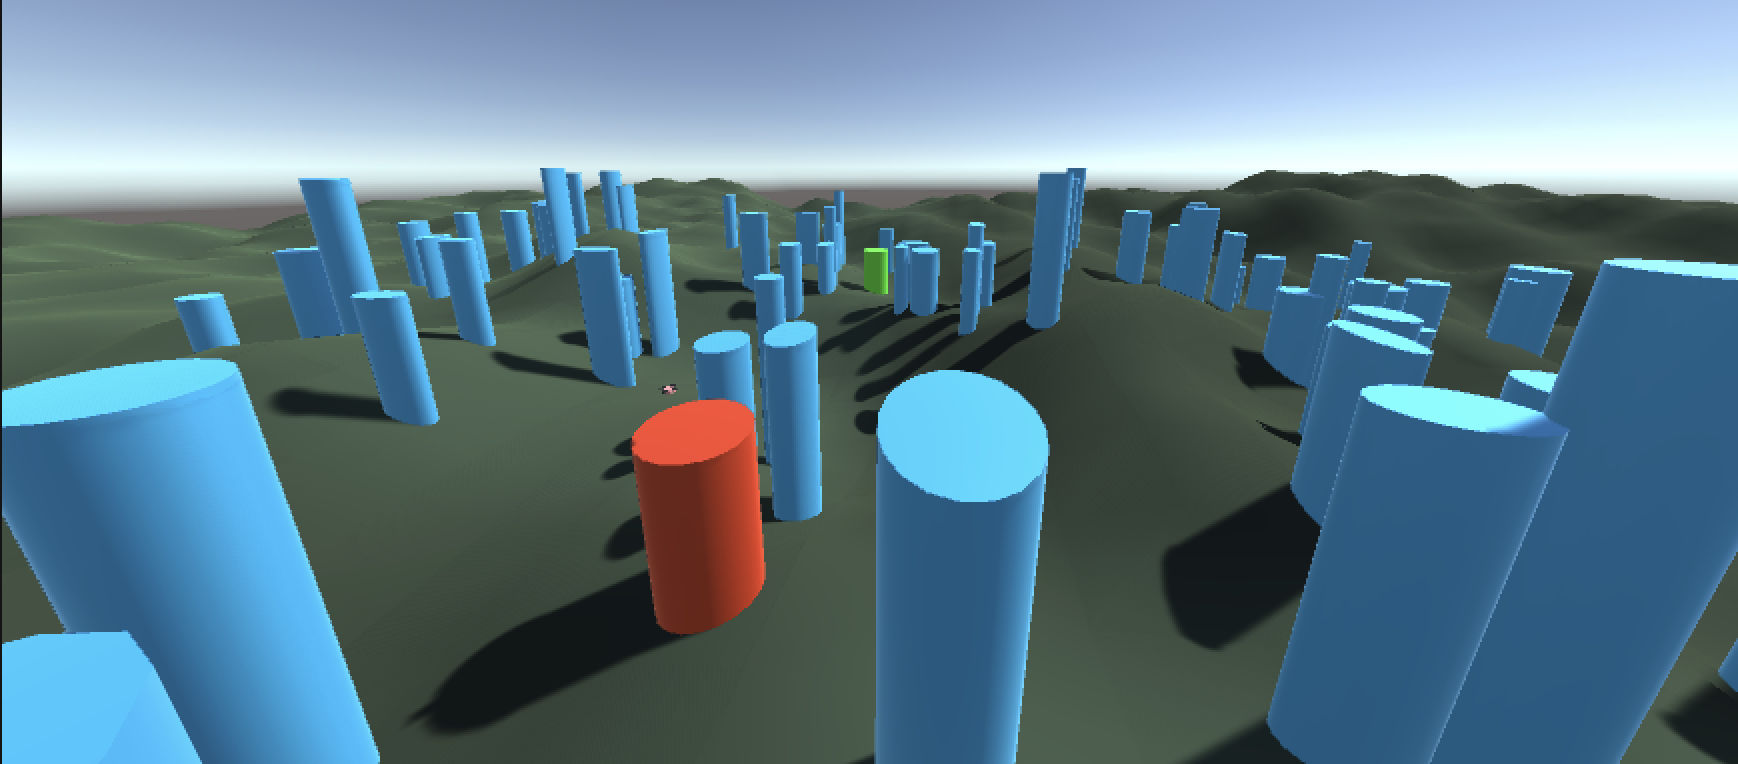
\includegraphics[width=0.8\textwidth]{obstacles.png}
    \caption{Obstacles in the Environment}
    \label{fig:obstacles}
\end{figure}

\subsection{A Simplified Model}
We now note that we have six behaviours with the aim of traversing a complex three-dimensional space. As noted earlier, the complexity of the parameter space increases exponentially with each additional parameter. Additionally, the relationship between the parameters and the emergent behaviour cannot be easily characterised, leading to difficulties in optimisation.

We now aim to reduce the complexity of the parameter space in the hopes of strengthening the link between the parameters and the emergent behaviour. For clarity, we reiterate the six behaviours as:

\begin{itemize}
    \item Avoidance
    \item Alignment
    \item Cohesion
    \item Seeking
    \item Terrain Avoidance
    \item Obstacle Avoidance
\end{itemize}

\subsubsection{Repulsion}
We notice that the nature of `avoiding' other objects in the simulation is shared across multiple behaviours. In theory, other agents could be considered as obstacles with a smaller range of avoidance. Likewise, the terrain could be considered as an obstacle with a larger range of avoidance. We can then look at combining these three behaviours into a single `repulsion' behaviour, with the general idea being that agents are repelled by other objects in the environment.

\subsubsection{Attraction}
On the contrary, the agents have some natural `attraction' to two main parts of the simulation. Primarily, the agents are attracted to the goal platform at longer distances. At shorter distances, the agents are additionally attracted to the centre of the flock. We can then look at combining the `seeking' and `cohesion' behaviours into a single `attraction' behaviour.

For now, we will not consider the `alignment' behaviour in this simplification, as it is not directly related to the `repulsion' or `attraction' behaviours.

\subsubsection{Combining Behaviours: Potential Fields}
Essentially, we have reduced the six behaviours into two behaviours which, in essence, encapsulate similar information. This refinement suggests that optimisation efforts can be more focused, essentially targeting these two key parameters. This approach draws a parallel with the concept of artificial potential fields, a foundational idea in robotics that illustrates the interplay between an agent and its surroundings. In this framework, agents are simultaneously drawn towards specific points of interest and repelled from obstacles, navigating the environment by moving in the direction of the net force exerted upon them.

We define the potential field, $U$, as the sum of the repulsion and attraction fields:

\begin{equation}
    U(x) = U_{rep}(x) + U_{att}(x)
\end{equation}

We can then define the repulsion field as:

\begin{equation}
    U_{rep}(x) = 
    \begin{cases}
        \frac{1}{2}k_r(\frac{1}{\rho}-\frac{1}{\rho_0}) & \text{if } \rho < \rho_0 \\
        0 & \text{otherwise}
    \end{cases}
\end{equation}

Namely, the repulsion field is a function of the distance between the agent and the obstacle, $\rho$, and the range of avoidance, $\rho_0$. The repulsion field is only active if the agent is within the range of avoidance. Similarly, we can define the attraction field as:

\begin{equation}
    U_{att}(x) = \frac{1}{2}k_a|x-x_d|^2
\end{equation}

We see that the attraction field is a function of the distance between the agent and the goal, $|x-x_d|$. The attraction field is always active. Notably, we can define the resultant force acting on the agent as the gradient of the potential field. More specifically, the negative derivative of the potential field:

\begin{equation}
    F_{rep}(x) = 
    \begin{cases}
        \frac{1}{2}k_r(\frac{1}{\rho}-\frac{1}{\rho_0})\frac{1}{\rho^2}\frac{\partial \rho}{\partial x} & \text{if } \rho < \rho_0 \\
        0 & \text{otherwise}
    \end{cases}
\end{equation}

\begin{equation}
    F_{att}(x) = -k_a(x-x_d)
\end{equation}

In the equations outlined, the coefficients \(k_r\) and \(k_a\) represent the weights for the repulsion and attraction forces, respectively. These weights are crucial parameters that require optimisation to fine-tune the interaction between the agent and its surroundings. Obstacles within the simulation environment, which include both static terrain features and dynamic entities like other agents, are assigned a specific radius, \(\rho_0\). This radius determines the threshold distance at which repulsion forces become active, thus preventing collisions by maintaining a safe distance between the agent and obstacles.

While it would be ideal to pre-calculate the potential fields and the resulting forces guiding agent movements, the dynamic nature of the simulation environment complicates this approach. Agents, serving as moving obstacles, constantly change the landscape of potential fields, rendering any pre-calculated forces obsolete within moments. Given this dynamic environment, calculating the resultant forces in real time becomes necessary. However, this approach is inherently computationally demanding, posing significant challenges, especially as the scale of the simulation environment and the number of agents increase.

To address these challenges, we propose an innovative method for online calculation of resultant forces that aims to minimise computational overhead. This method, which we will delve into in the following section, offers a practical solution for managing the complex dynamics of UAV swarms with greater efficiency and reduced computational resource requirements.

\subsection{Local Potential Field Emergence}
\label{sec:lpfe}
We can reduce the computational cost of calculating the resultant forces acting on the agents by only considering the forces acting on an agent within a certain radius. This is known as a \emph{local potential field}. We can then define the resultant force acting on an agent as the sum of the forces acting on the agent within a certain radius, $r$, such that $x_r$ defines the position of the agent and the influence radius $r$.

\begin{equation}
    F(x_r) = F_{att}(x_r) + F_{rep}(x_r)
\end{equation}

\subsubsection{Two Dimensional Abstraction}
Looking at the simulation environment along the $x$ and $z$ axes, we can produce a vector field to visualise some examples of what the force field may look like\footnote{As an aside, we note that the force field is a vector field, and the potential field can be represented as a scalar field. We use the vector field here, as it is easier to visualise.}.

Consider the attractive force, which considers two poles of attraction, one at the goal platform at $[-8,-8]$ and one at the centre of the flock at $[2,2]$. 

Here, we describe a position as $p = [x,z]$.

We can then define the force field as:

\begin{equation}
    F_{att}(p) = -k_{a1}(p-p_{goal}) - k_{a2}(p-p_{centre})
\end{equation}

We note that, because we represent multiple behaviours in the same attraction function, we have multiple weights, $k_{a1}$ and $k_{a2}$, for the two poles of attraction. These are equivalent to the weight of behaviours in the Boids implementation. We note that we can keep them equal to reduce the complexity of the environment. However, to ensure the agents are attracted to the goal platform at longer distances, we can set $k_{a1} > k_{a2}$. We will not explore tuning these values independently, as they should not relate to the repulsive behaviours.

\begin{figure}[ht]
    \centering
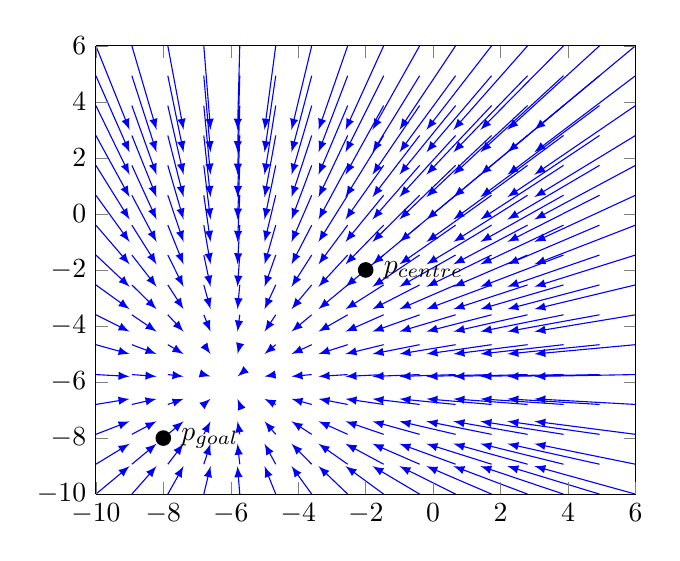
\begin{tikzpicture}
    \begin{axis}[%
     view     = {0}{90}, % for a view 'from above'
     domain   = -10:6,
     y domain = -10:6,
     xtick    = {-10,-8,...,6},
     ytick    = {-10,-8,...,6},
   ]
   \addplot3[blue, quiver={u=-1*(x-2)+-4*(x+8), v=-1*(y-2)+-4*(y+8), scale arrows=0.05}, samples=16, -latex] (x,y,0);
   \node[label={0:{$p_{goal}$}},circle,fill,inner sep=2pt] at (axis cs:-8,-8) {};
   \node[label={0:{$p_{centre}$}},circle,fill,inner sep=2pt] at (axis cs:-2,-2) {};

%    \addplot3[red, thick, domain=0:360, samples=41] ({0.5*sqrt(5)*cos(x)},{sqrt(5)*sin(x)},0);
   \end{axis}
   \end{tikzpicture}
    \caption{Attraction Force Field}
    \label{fig:force-field-att}
\end{figure}

Fig. \ref{fig:force-field-att} shows the force field for the attraction behaviour. We note that the pole of the field lies between both the goal platform and the centre of the flock. This is expected, as the agents should be attracted to both points. We could set a maximum distance for cohesion attraction, but this is not necessary for this simulation, as over time, we can see that the flock will naturally move towards the goal, due to having a higher weight in the attraction function. This is evident in the centre of the field, which is closer to the goal platform than the centre of the flock.

We can do the same for our repulsive behaviours. We do not consider the terrain as an obstacle in two dimensions, so will solely consider other agents, $\tau$, and the obstacles, $\rho$, in the environment. Hence, we can define the repulsive force field as:


\begin{equation}
    F_{rep}(p) = 
    \begin{cases}
        \frac{1}{2}k_r(\frac{1}{\rho}-\frac{1}{\rho_{0}})\frac{1}{\rho^2}\frac{\partial \rho}{\partial p} & \text{if } \rho < \rho_{0} \cap \tau > \tau_{0} \\
        \frac{1}{2}k_r(\frac{1}{\tau}-\frac{1}{\tau{0}})\frac{1}{\tau^2}\frac{\partial \tau}{\partial p} & \text{if } \rho > \rho_{0} \cap \tau < \tau_{0} \\
        \frac{1}{2}k_r(\frac{1}{\rho}-\frac{1}{\rho_{0}})\frac{1}{\rho^2}\frac{\partial \rho}{\partial p} + \frac{1}{2}k_r(\frac{1}{\tau}-\frac{1}{\tau{0}})\frac{1}{\tau^2}\frac{\partial \tau}{\partial p} & \text{if } \rho < \rho_{0} \cap \tau < \tau_{0} \\
        0 & \text{otherwise}
    \end{cases}
\end{equation}

We can then see the resulting repulsive force field in Fig. \ref{fig:force-field-rep}, with obstacles located at $[2,2]$ and $[5,5]$, with $\rho_0 = 1$, and another agent located at $[2,5]$, with $\tau_0 = 0.5$.

\begin{figure}[ht]
    \centering
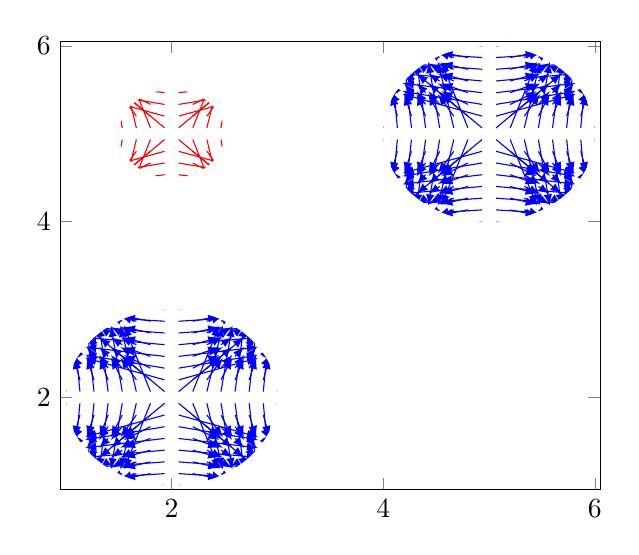
\begin{tikzpicture}
    \begin{axis}[%
     view     = {0}{90}, % for a view 'from above'
     domain   = -10:6,
     y domain = -10:6,
     xtick    = {-10,-8,...,6},
     ytick    = {-10,-8,...,6},
   ]
   \clip (5,5) circle (1) (2,2) circle (1) (2,5) circle (0.5);
   \addplot3[blue, quiver={u=1/(x-2), v=1/(y-2), scale arrows=0.05}, samples=16, -latex,domain=1:3,y domain=1:3] (x,y,0);
   \addplot3[blue, quiver={u=1/(x-5), v=1/(y-5), scale arrows=0.05}, samples=16, -latex,domain=4:6,y domain=4:6] (x,y,0);

   \addplot3[red, quiver={u=1/(x-2), v=1/(y-5), scale arrows=0.05}, samples=16, -latex,domain=1:3,y domain=4:6] (x,y,0);

%    \addplot3[red, thick, domain=0:360, samples=41] ({0.5*sqrt(5)*cos(x)},{sqrt(5)*sin(x)},0);
   \end{axis}
   \end{tikzpicture}
    \caption{Repulsion Force Field}
    \label{fig:force-field-rep}
\end{figure}

We can then combine these two fields to produce the resultant force field acting on the agents. We can then use this field to move the agents in the simulation environment.

The challenge with this model is that, whilst we have removed the complexity of the parameter space, we have introduced new parameters (such as the avoidance radius of the obstacles and other agents) which need to be optimised. However, unlike the arbitrary nature of the behaviour weightings, these parameters have a clear relationship with the behaviour of the agents in the environment. 

We then have the parameters $k_r$, $k_{a1}$, $k_{a2}$, $\rho_0$, and $\tau_0$ to optimise. With an extension into three dimensions, we would also have the parameter $\upsilon_0$ to consider, which would define the terrain avoidance distance. We could then use the simulated annealing algorithm to optimise these parameters, with the cost function being the same as before, but with the new parameters. This was determined to be out of scope for this project, where this novel alternative model was introduced as a potential solution to the issues faced in the previous section. 

\subsection{Comparing Models}
We can compare the Boids model with the LPFE model in terms of complexity and the relationship between the parameters and the emergent behaviour.

We note that the LPFE model is an extension of the Boids model, which, in theory, has more meaningful connections between the parameters and the observed behaviour. As such, we would expect the optimisation process to be more straightforward for the LPFE model than the Boids model. Specifically, we can expect the cost function to be more accurately characterised by the parameters in the LPFE model.

A comparison of the two models is shown in Table \ref{tab:model-comparison}.

\begin{table}[ht]
    \centering
    \begin{tabular}{|c|c|c|}
        \hline
       Feature & Boids & LPFE \\
        \hline\hline
        Number of Behaviours & 6 & 2 \\
        \hline
        Number of Parameters & 6 & 6 \\
        \hline
        Complexity of Parameter Space & High & Low \\
        \hline
        Parameter-Metric Relationship & Innacurate & More Accurate \\
        \hline
        Ease of Implementation & Easy & Hard \\
        \hline
    \end{tabular}
    \caption{Comparison of Boids and LPFE Models}
    \label{tab:model-comparison}
\end{table}

It is vital to note that as the LPFE model has not been implemented, the comparison is theoretical.

\newpage
\section{Future Work}
Whilst this project demonstrates the ability to use simulated annealing to optimise the parameters of a Boids simulation concerning given scenarios and the drawbacks of the method, there are several areas for future work. Namely, implementing the local potential field emergence model would be a good next step. We also explore increasing the complexity of the simulation to mirror real-life scenarios more accurately.

\subsection{LPFE Implementation}
Primarily, extending the model discussed in Section \ref{sec:lpfe} to three dimensions and performing simulations to test the viability of the model is a natural next step.

We can define the model in three dimensions by considering the position of the agent as $p = [x,y,z]$. We can then define the force field as the sum of the attractive forces acting on the agent and the repulsive forces acting on the agent within a certain radius, $r$. We would also include the terrain as an obstacle in the environment, with a similar avoidance radius to the other obstacles, represented by $\upsilon_0$, with the two force fields defined as:

\begin{equation}
    F_{att}(p) = -k_{a1}(p-p_{goal}) - k_{a2}(p-p_{centre})
\end{equation}

\begin{equation}
    F_{rep}(p) = 
    \begin{cases}
        \frac{1}{2}k_r(\frac{1}{\rho}-\frac{1}{\rho_{0}})\frac{1}{\rho^2}\frac{\partial \rho}{\partial p} & \text{if } \rho < \rho_{0} \cap \tau > \tau_{0} \cap \upsilon < \upsilon_{0}\\
        \frac{1}{2}k_r(\frac{1}{\tau}-\frac{1}{\tau_{0}})\frac{1}{\tau^2}\frac{\partial \tau}{\partial p} & \text{if } \rho > \rho_{0} \cap \tau < \tau_{0} \cap \upsilon < \upsilon_{0}\\
        \frac{1}{2}k_r(\frac{1}{\rho}-\frac{1}{\rho_{0}})\frac{1}{\rho^2}\frac{\partial \rho}{\partial p} + \frac{1}{2}k_r(\frac{1}{\tau}-\frac{1}{\tau_{0}})\frac{1}{\tau^2}\frac{\partial \tau}{\partial p} & \text{if } \rho < \rho_{0} \cap \tau < \tau_{0} \cap \upsilon < \upsilon_{0}\\
        \frac{1}{2}k_r(\frac{1}{\rho}-\frac{1}{\rho_{0}})\frac{1}{\rho^2}\frac{\partial \rho}{\partial p} + \frac{1}{2}k_r(\frac{1}{\upsilon}-\frac{1}{\upsilon_{0}})\frac{1}{\upsilon^2}\frac{\partial \upsilon}{\partial p} & \text{if } \rho < \rho_{0} \cap \tau > \tau_{0} \cap \upsilon > \upsilon_{0}\\
        \frac{1}{2}k_r(\frac{1}{\tau}-\frac{1}{\tau_{0}})\frac{1}{\tau^2}\frac{\partial \tau}{\partial p} + \frac{1}{2}k_r(\frac{1}{\upsilon}-\frac{1}{\upsilon_{0}})\frac{1}{\upsilon^2}\frac{\partial \upsilon}{\partial p} & \text{if } \rho > \rho_{0} \cap \tau < \tau_{0} \cap \upsilon > \upsilon_{0}\\
        \frac{1}{2}k_r(\frac{1}{\rho}-\frac{1}{\rho_{0}})\frac{1}{\rho^2}\frac{\partial \rho}{\partial p} + \frac{1}{2}k_r(\frac{1}{\tau}-\frac{1}{\tau_{0}})\frac{1}{\tau^2}\frac{\partial \tau}{\partial p} + \frac{1}{2}k_r(\frac{1}{\upsilon}-\frac{1}{\upsilon_{0}})\frac{1}{\upsilon^2}\frac{\partial \upsilon}{\partial p} & \text{if } \rho < \rho_{0} \cap \tau < \tau_{0} \cap \upsilon > \upsilon_{0}\\
        0 & \text{otherwise}
    \end{cases}
\end{equation}

We would then perform simulations to test the viability of the model. This would involve testing the model in a variety of environments, with different obstacles and terrain, to ensure the model is robust. Once this has been completed, we can then look at optimising the parameters of the model, specifically $k_r,k_{a1},k_{a2}$, using the simulated annealing algorithm.

Following this implementation, we can then compare the LPFE model to the Boids model in terms of complexity and the relationship between the parameters and the emergent behaviour. This would allow exploration of the effectiveness of the LPFE model in comparison to the Boids model.

\subsection{Other Models}
The simulated annealing optimisation model is only one out of many methods of determining an optimal parameter set. Here, we discuss the set of possible alternative methods for optimisation in our specific problem.

\subsubsection{Online Optimisation}
The models we have explored have fixed parameters which are determined before a simulation run. One possible avenue of exploration is looking at online parameter optimisation. Some parameters are likely more important and as such, should have higher weightings, at different points in a simulation. For example, looking at the Boids model, we can expect the need for seeking to be higher the further away the agent is from the goal. Likewise, in life-like scenarios, we would expect the agents to have a stronger avoidance weight when they are expected to be closer together, such as when leaving the start area or near the goal area.

The lack of this behaviour meant collisions occurred more frequently near the goal platform in the simulated annealing process; this is seen in Fig. \ref{fig:collisions-goal}. As discussed earlier, we would expect the avoidance behaviour to have an inverse correlation with the number of collisions, thus, this may have thrown off the annealing process.

\begin{figure}[ht]
    \centering
    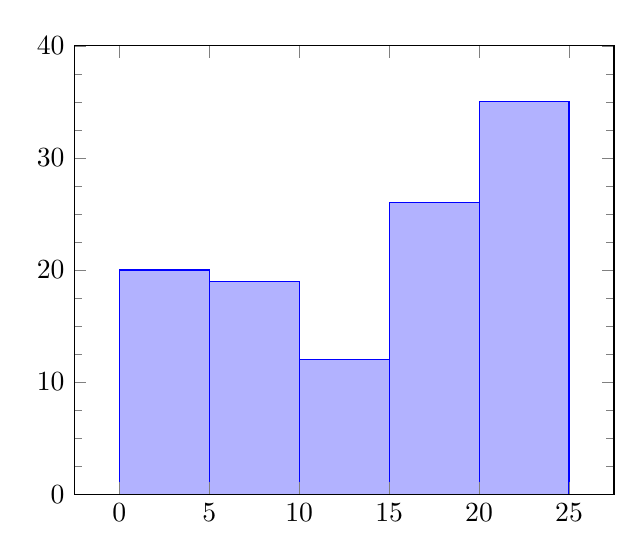
\begin{tikzpicture}
        \begin{axis}[
            ymin=0, ymax=40,
            minor y tick num = 3,
            area style,
            ]
        \addplot+[ybar interval,mark=no] plot coordinates { (0, 20) (5, 19) (10, 12) (15, 26) (20, 35) (25, 33) };
        \end{axis}
        \end{tikzpicture}
    \caption{Number of Collisions (First agent reaching the goal at $t\approx 25$)}
    \label{fig:collisions-goal}
\end{figure}

\subsubsection{Neural Network Optimisaton}
A more complex learning technique, the use of a neural network, would likely have the ability to converge to a global minimum more accurately. While the promise of neural networks is enticing, their integration into real-time simulation environments is hampered by substantial computational demands. Training neural networks, especially deep models, requires significant computational resources and time, which might not be feasible in scenarios requiring quick adaptations. Additionally, the implementation of such models in a dynamically changing environment adds another layer of complexity due to the need for continual retraining or fine-tuning as new data becomes available.

The use of neural networks in the context of optimisation is not new; \citet{Caldwell} introduce a method of utilising deep neural networks for combinatorial optimisation, which could be adapted to solving the parameter optimisation problem in this project. Notably, as mentioned earlier, optimisation problems require appropriate parameter selection - a difficult task which may be alleviated by the use of neural networks. \citet{zhao2022nature} use a \emph{reward modulated spiking neural network} to allow a flock to learn to avoid obstacles, rather than using a pre-defined set of rules.

\subsection{Hostility}
An interesting extension to the Boids model is the introduction of hostile agents and environments. This would likely require a more complex model, as the agents would need to be able to detect the hostility and react accordingly. We discuss potential methods for this here.

\subsubsection{Hostile Agents}
We may consider the introduction of agents which are hostile to the flock. This could be implemented by having the hostile agents move towards the flock, with the flock needing to avoid them; a concept which has been explored with the Boids model\cite{chen2008application}.

\citet{delgado2007use} modify the Boids model to include an `escape' behaviour, where the flock moves away from a hostile agent. Additionally, the model uses the concept of `fear contagion', where the flock is more likely to move away from hostility if neighbouring agents are moving away from said hostility. 

An example implementation of this may include the introduction of a hostile agent with the seeking behaviour tailored to the centre of the flock. The flock would have a method of detecting hostile agents, similar to the obstacle avoidance behaviour. We may then choose to add the element of fear contagion, where an agent's fear is dependent on the fear of its neighbours. Namely,

\begin{equation}
    F_{fear}(a) = -k_{fear}(a-a_{centre})
\end{equation}

An agent's fear may also be determined by the number of hostile agents within an agent's avoidance radius. Attempting to optimise this additional parameter would serve as a potential extension to the Boids model.

Additionally, the hostile agents could have the ability to attack the flock from a distance with projectiles, which would require the flock to avoid the projectiles as well as the agents. Incorporating the ability to detect and avoid projectiles would bring this model closer to real-life scenarios.


\subsubsection{Hostile Environments}
In addition to hostile agents, the possibility of varying environmental conditions could be explored. For example, environments where there are more complex obstacles, such as narrow corridors, or environments where the terrain is more difficult to traverse. This would require the flock to adapt to the environment and change their behaviour accordingly. 

We may consider the introduction of temperature, precipitation, humidity, and wind speed to the model, which would affect the flock's behaviour.  An implementation of this may focus on modifying the world generation with the introduction of biomes; \citet{jiang2017biome,whittaker1970communities} note the common classification of biomes from precipitation and temperature, which could be extended to include other environmental factors.

To complement this, we may also simulate an agent's battery and signal strength when navigating the environment. As a result, the environmental conditions would affect the agent's signal strength and battery life, which should be considered when optimising the parameters of the model. Discussing more scenarios dependent on the environment in this way may increase the robustness of the model. Additionally, simulating the communication between agents and the effect of the environment on this communication would bring the model closer to a realistic simulation, as described by \citet{Zhou}.

\section{Evaluation}
This section evaluates the project as a whole, discussing the successes and failures of the project and some key remarks.

\subsection{Project Management}
In the initial stages of planning, a Gantt chart was produced to outline the project timeline. This can be seen in Fig. \ref{fig:gantt-eval}. 

\begin{figure}[ht]
    \centering
    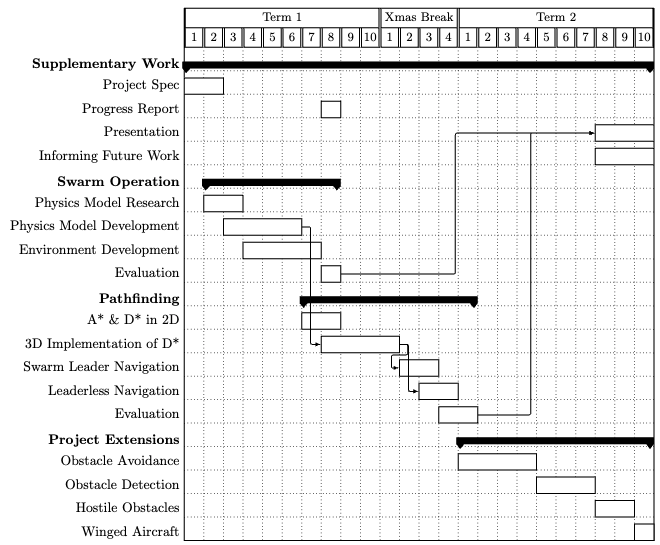
\includegraphics[width=0.8\textwidth]{gantt.png}
    \caption{Gantt Chart}
    \label{fig:gantt-eval}
\end{figure}

Breaking down the key sections of the project into smaller tasks allowed for a more manageable project. Looking at the Gantt chart, we note the modifications in the project timeline below.

\subsubsection{Project Timeline Modifications}
The largest change to the timeline was the shift in focus over the Christmas break. Initially, the focus after finishing the operation of the Boids model and the agent control system was to focus on exploring and comparing pathfinding algorithms for the Boids model.

The reasoning behind this initial plan was to explore how different pathfinding algorithms, such as A*, could affect the behaviour of the agents in the Boids model. Additionally, the exploration of `leadership' in the flock was planned. Instead, the focus shifted to optimising the emergent behaviour of the Boids model. This was due to the complexity of the pathfinding algorithms, particularly in three dimensions.

The Gantt chart was planned in a way that allowed for plenty of contingency time in the latter half of the project, in case of any delays or issues. Whilst this meant that some of the `extensions' to the project were late, such as the exploration of obstacle detection and avoidance, whilst others were not completed, such as the exploration of hostile agents and environments, the project was completed on time. As such, this was a successful strategy.

The actual progress of the project can be seen in Fig. \ref{fig:gantt-actual}.

\begin{figure}[ht]
    \begin{center}
    
    \begin{ganttchart}[y unit title=0.5cm,
    y unit chart=0.6cm,
    vgrid,hgrid, 
    title label anchor/.style={below=-1.6ex},
    title left shift=.05,
    title right shift=-.05,
    title height=1,
    progress label text={},
    bar height=0.7,
    group right shift=0,
    group top shift=.6,
    group height=.3,
    group peaks height=.2,
    link mid=.45]{1}{24}
    %labels
    \gantttitle{Term 1}{10}
    \gantttitle{Xmas Break}{4}
    \gantttitle{Term 2}{10} \\
    \gantttitle{1}{1} 
    \gantttitle{2}{1} 
    \gantttitle{3}{1} 
    \gantttitle{4}{1} 
    \gantttitle{5}{1}
    \gantttitle{6}{1} 
    \gantttitle{7}{1} 
    \gantttitle{8}{1} 
    \gantttitle{9}{1} 
    \gantttitle{10}{1}
    \gantttitle{1}{1} %week 11
    \gantttitle{2}{1} 
    \gantttitle{3}{1} 
    \gantttitle{4}{1} 
    \gantttitle{1}{1} %week 15
    \gantttitle{2}{1} 
    \gantttitle{3}{1} 
    \gantttitle{4}{1} 
    \gantttitle{5}{1}
    \gantttitle{6}{1} %week 20
    \gantttitle{7}{1} 
    \gantttitle{8}{1} 
    \gantttitle{9}{1} 
    \gantttitle{10}{1} \\
    %tasks
    \ganttgroup{Supp. Work}{1}{24} \\
    \ganttbar{Project Spec}{1}{2} \\
    \ganttbar{Progress Report}{8}{8} \\
    \ganttbar{Presentation}{24}{24} \\
    \ganttbar{Future Work}{24}{24} \\

    \ganttgroup{Swarm}{2}{11} \\
    \ganttbar{Physics Model}{2}{6} \\
    \ganttbar{Boids Model}{7}{10} \\
    \ganttbar{Boids Extension}{10}{13} \\
    \ganttbar{Evaluation}{14}{15} \\

    \ganttgroup{Optimisation}{15}{23} \\
    \ganttbar{Research}{15}{16} \\
    \ganttbar{Simulated Annealing}{17}{22} \\
    \ganttbar{Evaluation}{22}{23} \\

    \ganttgroup{Extensions}{22}{24} \\
    \ganttbar{Obstacle Avoidance}{22}{23} \\
    \ganttbar{LPFE Model}{23}{24}

    \ganttlink{elem7}{elem12}
    \ganttlink{elem8}{elem12}
    \ganttlink{elem13}{elem3}
    \ganttlink{elem9}{elem3}


    \end{ganttchart}
    \end{center}
    \caption{Gantt Chart of Actual Progress}
    \label{fig:gantt-actual}
\end{figure}


\subsubsection{Methodology}
The project was conducted in a way that allowed for a clear progression from the initial exploration of the Boids model to the optimisation of the model. As a single-person project, the development process followed a waterfall model, with each stage of the project being completed before moving on to the next stage. This was a successful strategy, as it allowed for a clear progression of the project. In a multi-person project, this method may not be suitable, as some team members may have a lot of idle time whilst waiting for others to complete their tasks.

The breakdown of the time spent on the project, broken down per week, can be seen in Table \ref{tab:time-breakdown}. Weeks 11-14 in both terms were the Christmas and Easter breaks, respectively. The table shows an average of $\approx 10$ hours per week spent on the project, with a total time of 250 hours spent on the project. This does not include reading time, supervisor meetings, peer consultations or relevant lectures. The addition of these would likely bring the total time spent on the project to $\approx 300$ hours.

\begin{table}[ht]
    \centering
    \begin{tabular}{|c|c||c|c|}
        \hline
        Week & Hours & Week & Hours \\
        \hline
        1 & 3 & 1 & 6 \\
        2 & 10 & 2 & 7 \\
        3 & 25 & 3 & 9 \\
        4 & 13 & 4 & 8 \\
        5 & 10 & 5 & 10 \\
        6 & 12 & 6 & 8 \\
        7 & 7 & 7 & 11 \\
        8 & 2 & 8 & 17 \\
        9 & 5 & 9 & 16 \\
        10 & 5 & 10 & 6 \\
        11 & 0 & 11 & 44 \\
        12 & 0 & 12 & 16 \\
        13 & 0 & 13 & 0 \\
        14 & 16 & 14 & 0 \\
        \hline
    \end{tabular}
    \caption{Time Breakdown}
    \label{tab:time-breakdown}
\end{table}

\subsubsection{Contingency Planning}
As noted previously, the planned timeline allowed for plenty of contingency time in the latter half of the project. Complementary to this was the use of Github, which allowed for easy tracking of changes and the ability to revert to previous versions of the code. Github also allowed for the entire project to be stored remotely. This meant that the project was not lost in the event of a hardware failure, misplacement or theft; a real concern, as part of the project was completed abroad and required frequent travel between locations.

Keeping track of the tasks completed weekly meant this reflection was possible. This allowed for a clear understanding of the project progression and the ability to identify areas where more time could have been spent. 


\subsection{Remarks: Assumptions}
Though this report has focused on the optimisation of a parameter space to achieve emergent behaviour in a Boids model, several assumptions were left untweaked to simplify the model.

Much of the parameters of the flock generation were kept constant. Exploring how the flock size, avoidance radius and other parameters affect the emergent behaviour of the flock would be an interesting extension to this project. Likewise, the PID controller used to control the agents was kept constant. Exploring how the parameters of the PID controller affect the emergent behaviour of the flock could be explored.

Generally, there will always be some trade-off between some of these parameters we have kept constant. Reducing the number of agents in the simulation would likely reduce the number of collisions, but the effect of the cohesion behaviour, for example, would be more difficult to explore. Likewise, increasing the maximum tilt in the PID controller could have led to a faster convergence to the goal, but could have led to more collisions, oscillations and likely a more noisy simulation.

\subsection{Author's Assessment of the Project}


Overall, this project has been a success. The project has explored the optimisation of a Boids model using simulated annealing, a relevant and important topic in the field of artificial intelligence and the wider field of computer science. The project has also introduced a novel extension to the Boids model, the Local Potential Field Emergence model.

The project has not explored the optimisation of the LPFE model, which would have been a natural extension of the project.

Hopefully, the project can be used as a basis for further exploration into the optimisation of emergent behaviour in agent-based models, specifically in a world-like environment.

\newpage
\section*{Acknowledgments}
This project's success would not have been possible without the support of my supervisor, Nathan Griffiths, who provided guidance and support throughout the project. Additionally, Dr. Claire Rocks provided a welcome second opinion on some initial ideas for the project's direction and Arpan Mukhopadhyay, who sparked valuable ideas from his questions and comments. I would also like to thank my peers, who provided valuable explanation, feedback, discourse and support throughout the project, namely Christopher Wilkinson, Ethan Larkin, Luke Sarfas and Maddie Sangway.

\newpage
\bibliographystyle{IEEEtranN}
\bibliography{refs} 
\end{document}

